%%%%%%%%%%%%%%%%%%%%%%%%%%%%%%%%%%%%%%%%%
% Masters/Doctoral Thesis 
% LaTeX Template
% Version 2.4 (22/11/16)
%
% This template has been downloaded from:
% http://www.LaTeXTemplates.com
%
% Version 2.x major modifications by:
% Vel (vel@latextemplates.com)
%
% This template is based on a template by:
% Steve Gunn (http://users.ecs.soton.ac.uk/srg/softwaretools/document/templates/)
% Sunil Patel (http://www.sunilpatel.co.uk/thesis-template/)
%
% Template license:
% CC BY-NC-SA 3.0 (http://creativecommons.org/licenses/by-nc-sa/3.0/)
%
%%%%%%%%%%%%%%%%%%%%%%%%%%%%%%%%%%%%%%%%%

%----------------------------------------------------------------------------------------
%	PACKAGES AND OTHER DOCUMENT CONFIGURATIONS
%----------------------------------------------------------------------------------------

\documentclass[
11pt, % The default document font size, options: 10pt, 11pt, 12pt
oneside, % Two side (alternating margins) for binding by default, uncomment to switch to one side
english, % ngerman for German
singlespacing, % Single line spacing, alternatives: onehalfspacing or doublespacing
%draft, % Uncomment to enable draft mode (no pictures, no links, overfull hboxes indicated)
%nolistspacing, % If the document is onehalfspacing or doublespacing, uncomment this to set spacing in lists to single
%liststotoc, % Uncomment to add the list of figures/tables/etc to the table of contents
%toctotoc, % Uncomment to add the main table of contents to the table of contents
%parskip, % Uncomment to add space between paragraphs
%nohyperref, % Uncomment to not load the hyperref package
headsepline, % Uncomment to get a line under the header
chapterinoneline, % Uncomment to place the chapter title next to the number on one line
%consistentlayout, % Uncomment to change the layout of the declaration, abstract and acknowledgements pages to match the default layout
]{MastersDoctoralThesis} % The class file specifying the document structure

\usepackage[utf8]{inputenc} % Required for inputting international characters
\usepackage[T1]{fontenc} % Output font encoding for international characters

\usepackage{palatino} % Use the Palatino font by default

\usepackage{tikz}
\usepackage[utf8]{inputenc}
\usetikzlibrary{matrix,shapes,arrows,positioning,chains}
\usepackage{adjustbox}
\usepackage{amsmath}


\usepackage[backend=bibtex,style=authoryear,natbib=true]{biblatex} % Use the bibtex backend with the authoryear citation style (which resembles APA)

\addbibresource{example.bib} % The filename of the bibliography

\usepackage[autostyle=true]{csquotes} % Required to generate language-dependent quotes in the bibliography

\usepackage{listings}
\usepackage{color}

\definecolor{dkgreen}{rgb}{0,0.6,0}
\definecolor{gray}{rgb}{0.5,0.5,0.5}
\definecolor{mauve}{rgb}{0.58,0,0.82}

\lstset{frame=tb,
	language=C++,
	aboveskip=3mm,
	belowskip=3mm,
	showstringspaces=false,
	columns=flexible,
	basicstyle={\small\ttfamily},
	numbers=none,
	numberstyle=\tiny\color{gray},
	keywordstyle=\color{blue},
	commentstyle=\color{dkgreen},
	stringstyle=\color{mauve},
	breaklines=true,
	breakatwhitespace=true,
	tabsize=3
}

%----------------------------------------------------------------------------------------
%	MARGIN SETTINGS
%----------------------------------------------------------------------------------------

\geometry{
	paper=a4paper, % Change to letterpaper for US letter
	inner=2.5cm, % Inner margin
	outer=2.5cm, % Outer margin
	%bindingoffset=.5cm, % Binding offset
	top=1.5cm, % Top margin
	bottom=1.5cm, % Bottom margin
	%showframe, % Uncomment to show how the type block is set on the page
}

%----------------------------------------------------------------------------------------
%	THESIS INFORMATION
%----------------------------------------------------------------------------------------

\thesistitle{Mobile Scanner} % Your thesis title, this is used in the title and abstract, print it elsewhere with \ttitle
\degree{Master of Engineering in Robotics} % Your degree name, this is used in the title page and abstract, print it elsewhere with \degreename
\author{Lakshman Kumar K N} % Your name, this is used in the title page and abstract, print it elsewhere with \authorname
\addresses{} % Your address, this is not currently used anywhere in the template, print it elsewhere with \addressname

\subject{Digital Image and Video Processing} % Your subject area, this is not currently used anywhere in the template, print it elsewhere with \subjectname
\keywords{} % Keywords for your thesis, this is not currently used anywhere in the template, print it elsewhere with \keywordnames
\university{ENEE631} % Your university's name and URL, this is used in the title page and abstract, print it elsewhere with \univname
\department{Maryland Robotics Center} % Your department's name and URL, this is used in the title page and abstract, print it elsewhere with \deptname
\faculty{\href{http://faculty.university.com}{Faculty Name}} % Your faculty's name and URL, this is used in the title page and abstract, print it elsewhere with \facname

\AtBeginDocument{
\hypersetup{pdftitle=\ttitle} % Set the PDF's title to your title
\hypersetup{pdfauthor=\authorname} % Set the PDF's author to your name
\hypersetup{pdfkeywords=\keywordnames} % Set the PDF's keywords to your keywords
}

\begin{document}

\frontmatter % Use roman page numbering style (i, ii, iii, iv...) for the pre-content pages

\pagestyle{plain} % Default to the plain heading style until the thesis style is called for the body content

%----------------------------------------------------------------------------------------
%	TITLE PAGE
%----------------------------------------------------------------------------------------

\begin{titlepage}
\begin{center}

\vspace*{.06\textheight}
{\scshape\LARGE \univname\par}\vspace{1.5cm} % University name
\textsc{\Large \subjectname}\\[0.5cm] % Thesis type

\HRule \\[0.4cm] % Horizontal line
{\huge \bfseries \ttitle\par}\vspace{0.4cm} % Thesis title
\HRule \\[1.5cm] % Horizontal line
 
\begin{minipage}[t]{0.4\textwidth}
\end{minipage}
\begin{minipage}[t]{0.4\textwidth}

\end{minipage}\\[3cm]
 
\vfill

 \large
\emph{Author:}\\
\authorname
\\[0.3cm] % University requirement text
\degreename\\\deptname\\[2cm] % Research group name and department name
 
\vfill

{\large May 16, 2017}\\[1cm] % Date
%\includegraphics{Logo} % University/department logo - uncomment to place it
 
\vfill
\end{center}
\end{titlepage}

%----------------------------------------------------------------------------------------
%	DECLARATION PAGE
%----------------------------------------------------------------------------------------

\begin{declaration}
\addchaptertocentry{\authorshipname} % Add the declaration to the table of contents
\noindent I, \authorname, declare that this project report titled, \enquote{\ttitle} and the work presented in it are my own. I confirm that:

\begin{itemize} 
\item This work was done wholly for the course ENEE631 - Digital Image and Video Processing at the University of Maryland, College Park.
\item Where I have consulted the published work of others, this is always clearly attributed.
\item Where I have quoted from the work of others, the source is always given. With the exception of such quotations, this project is entirely my own work.
\item I have acknowledged all main sources of help.
\\
\end{itemize}

\begin{minipage}[t]{0.8\textwidth}
\end{minipage}
\begin{minipage}[t]{0.8\textwidth}
	
\end{minipage}\\[3cm]
 
\noindent Signed:\\
\rule[0.5em]{25em}{0.5pt} % This prints a line for the signature
 
\noindent Date: \ \ \ \ \  May 16, 2017\\
\rule[0.5em]{25em}{0.5pt} % This prints a line to write the date
\end{declaration}

\cleardoublepage

%----------------------------------------------------------------------------------------
%	ABSTRACT PAGE
%----------------------------------------------------------------------------------------

\begin{abstract}
\addchaptertocentry{\abstractname} % Add the abstract to the table of contents
Cell phones have become an integral part of our life. These devices are now being used to scan a document with its camera. This project attempts to model and implement the technique, by which a document is being scanned by a cell phone's camera and being registered to extract text from a filled form, used by several mobile scanner applications in the digital app stores of cell phones. The modeled technique was then tested on several images and the results were found to be almost close to the output of popular mobile scanner applications. The said techniques comprises of algorithms such as Canny Edge Detection, Border Following based Contour Estimation, ORB Feature Detection/Matching, Harris Corner Detection, Gaussian Minus C Adaptive Thresholding etc.
\end{abstract}

%----------------------------------------------------------------------------------------
%	LIST OF CONTENTS/FIGURES/TABLES PAGES
%----------------------------------------------------------------------------------------

\tableofcontents % Prints the main table of contents

\listoffigures % Prints the list of figures

%----------------------------------------------------------------------------------------
%	ABBREVIATIONS
%----------------------------------------------------------------------------------------

\begin{abbreviations}{ll} % Include a list of abbreviations (a table of two columns)

\textbf{OCR} & \textbf{O}ptical \textbf{C}haracter \textbf{R}ecognition\\
\textbf{FAST} & \textbf{F}eatures from  \textbf{A}ccelerated \textbf{S}egment \textbf{T}est\\
\textbf{BRIEF} & \textbf{B}inary  \textbf{R}obust \textbf{I}ndependent \textbf{E}lementary \textbf{F}eatures\\

\textbf{ORB} & \textbf{O}riented FAST and \textbf{R}otated \textbf{B}RIEF \\
\textbf{API} & \textbf{A}pplication \textbf{P}rogramming \textbf{I}nterface \\
\textbf{KNN} & \textbf{K} \textbf{N}earest \textbf{N}eighbor \\
\textbf{SIFT} & \textbf{S}cale \textbf{I}nvariant \textbf{F}eature \textbf{T}ransform \\
\textbf{SURF} & \textbf{S}peeded  \textbf{U}p \textbf{R}obust \textbf{F}eatures\\

\textbf{RANSAC} & \textbf{RAN}dom \textbf{SA}mple \textbf{C}onsensus \\

\end{abbreviations}

%---------------------------t-------------------------------------------------------------
%	THESIS CONTENT - CHAPTERS
%----------------------------------------------------------------------------------------

\mainmatter % Begin numeric (1,2,3...) page numbering

\pagestyle{thesis} % Return the page headers back to the "thesis" style

% Include the chapters of the thesis as separate files from the Chapters folder
% Uncomment the lines as you write the chapters

% Chapter 1

\chapter{Overview} % Main chapter title

\label{Chapter1} % For referencing the chapter elsewhere, use \ref{Chapter1} 

%------------------------------------------------------------------------

% Define some commands to keep the formatting separated from the content 
\newcommand{\keyword}[1]{\textbf{#1}}
\newcommand{\tabhead}[1]{\textbf{#1}}
\newcommand{\code}[1]{\texttt{#1}}
\newcommand{\file}[1]{\texttt{\bfseries#1}}
\newcommand{\option}[1]{\texttt{\itshape#1}}

%------------------------------------------------------------------------

\section{Introduction}
With increasing prevalence of cell phones among all the people, traditional devices, that have been used for various functions, are being replaced by cell phones. One such device is the scanner, which has been traditionally used to scan paper documents like forms, receipts, ID's. As the cell phone has a camera in it, the images of paper documents can be captured by it and advanced image processing techniques can be used to extract the document properly. The methodology behind document extraction from camera images and image registration has been implemented and analyzed as a part of this project.

%----------------------------------------------------------------------------------------

\section{Problem Statement}

The goal of the project is to implement and investigate the techniques that goes behind extracting a document from a mobile phone's image. Apart from just extracting the document, an enhanced functionality, that allows for image registration of a reference blank page and extraction of the filled content, has to be implemented.
 
\section{Assumptions Made}
\label{Assumptions}
\begin{itemize}
  \item The reference document is captured in a well lit and contrasting environment.
  \item The reference document is rectangular and convex.
  \item The reference document's 4 edges and 4 corners are clearly visible.
  \item The reference document occupies the most area in the captured image.
  \item The document with filled content has sufficient features.
\end{itemize}

\section{Related Works}

Various mobile scanning apps, like CamScanner, ScanBot, Evernote Scannable, Turbo Scan, are now available on app stores of Android, Apple and Windows phones. These apps include various sophisticated features, like OCR, Text Extraction, Image Annotation, Document Categorization etc., apart from the basic document extraction functionality .




% Chapter 2
 % For referencing the chapter elsewhere, use \ref{Chapter1}
%\begin{figure}
\chapter{Document Extraction} % Main chapter title
\label{Chapter2}
%----------------------------------------------------------------------------------------

\section{Flow Chart}
\nopagebreak
% Define block styles
\tikzset{
	desicion/.style={
		diamond,
		draw,
		text width=6em,
		text badly centered,
		inner sep=0pt
	},
	block/.style={
		rectangle,
		draw,
		text width=15em,
		text centered,
		rounded corners
	},
	cloud/.style={
		draw,
		ellipse,
		minimum height=1em
	},
	descr/.style={
		fill=white,
		inner sep=2.5pt
	},
	connector/.style={
		-latex,
		font=\scriptsize
	},
	rectangle connector/.style={
		connector,
		to path={(\tikztostart) -- ++(#1,0pt) \tikztonodes |- (\tikztotarget) },
		pos=0.5
	},
	rectangle connector/.default=-2cm,
	straight connector/.style={
		connector,
		to path=--(\tikztotarget) \tikztonodes
	}
}
\begin{center}
	\begin{figure}[hbt]
		\centering
	\begin{tikzpicture}
\matrix (m)[matrix of nodes, column  sep=2cm,row  sep=8mm, align=center, nodes={rectangle,draw, anchor=center} ]{
	|[block]| {Start}              &  \\
	|[block]| { Capture the image \\ of the document }               &                                            \\
	|[desicion]| {Image greater than 640 X 480 ?}          & |[block]| {Resize image by the scale factor based on the ratio between the size of the image and 640 X 480}                                               \\
	|[block]| {Convert to grayscale and enhance image by \\ Sharpening, Bilateral Filtering}    &                                             \\
	|[block]| {Canny Edge Detection}    &            |[block]| {Stop}                                   \\
	|[block]| {Fill small holes by Erosion/Dilation}    &    |[block]| {Do adaptive thresholding to create a binary image}                                          \\
	|[block]| {Extract biggest rectangular \\ convex contour}        &       |[block]| {Warp the image using the perspective transform and do bilinear interpolation}                                      \\
	|[block]| {Extract corners using \\ Harris Corner Detector and order the corners in clockwise direction}    &   |[block]| {Upscale corners to original size and extract perspective \\transform between this \\ polygon and an ideal rectangle }                                         \\
};
\path [>=latex,->] (m-1-1) edge (m-2-1);
\path [>=latex,->] (m-2-1) edge (m-3-1);
\path [>=latex,->] (m-3-1) edge node[auto] {\scriptsize{NO}} (m-4-1);
\path [>=latex,->] (m-3-1) edge node[auto] {\scriptsize{YES}} (m-3-2);
\draw [>=latex,->] (m-3-2) |- (m-4-1);
\path [>=latex,->] (m-4-1) edge (m-5-1);
\path [>=latex,->] (m-5-1) edge (m-6-1);
\path [>=latex,->] (m-6-1) edge (m-7-1);
\path [>=latex,->] (m-7-1) edge (m-8-1);
\path [>=latex,->] (m-8-1) edge (m-8-2);
\path [>=latex,->] (m-8-2) edge (m-7-2);
\path [>=latex,->] (m-7-2) edge (m-6-2);
\path [>=latex,->] (m-6-2) edge (m-5-2);

\end{tikzpicture}
    \caption{Flow Chart for Document Extraction}
\label{fig:DocumentExtractionFlowChart}
\end{figure}
\end{center}
%\caption[Document Extraction]{Flowchart for Document Extraction.}


%\end{figure}

\section{Document Extraction Techniques}

Consider the image shown below from which the document is to be extracted. 
\\ \\

\begin{figure}[th]
	\centering
	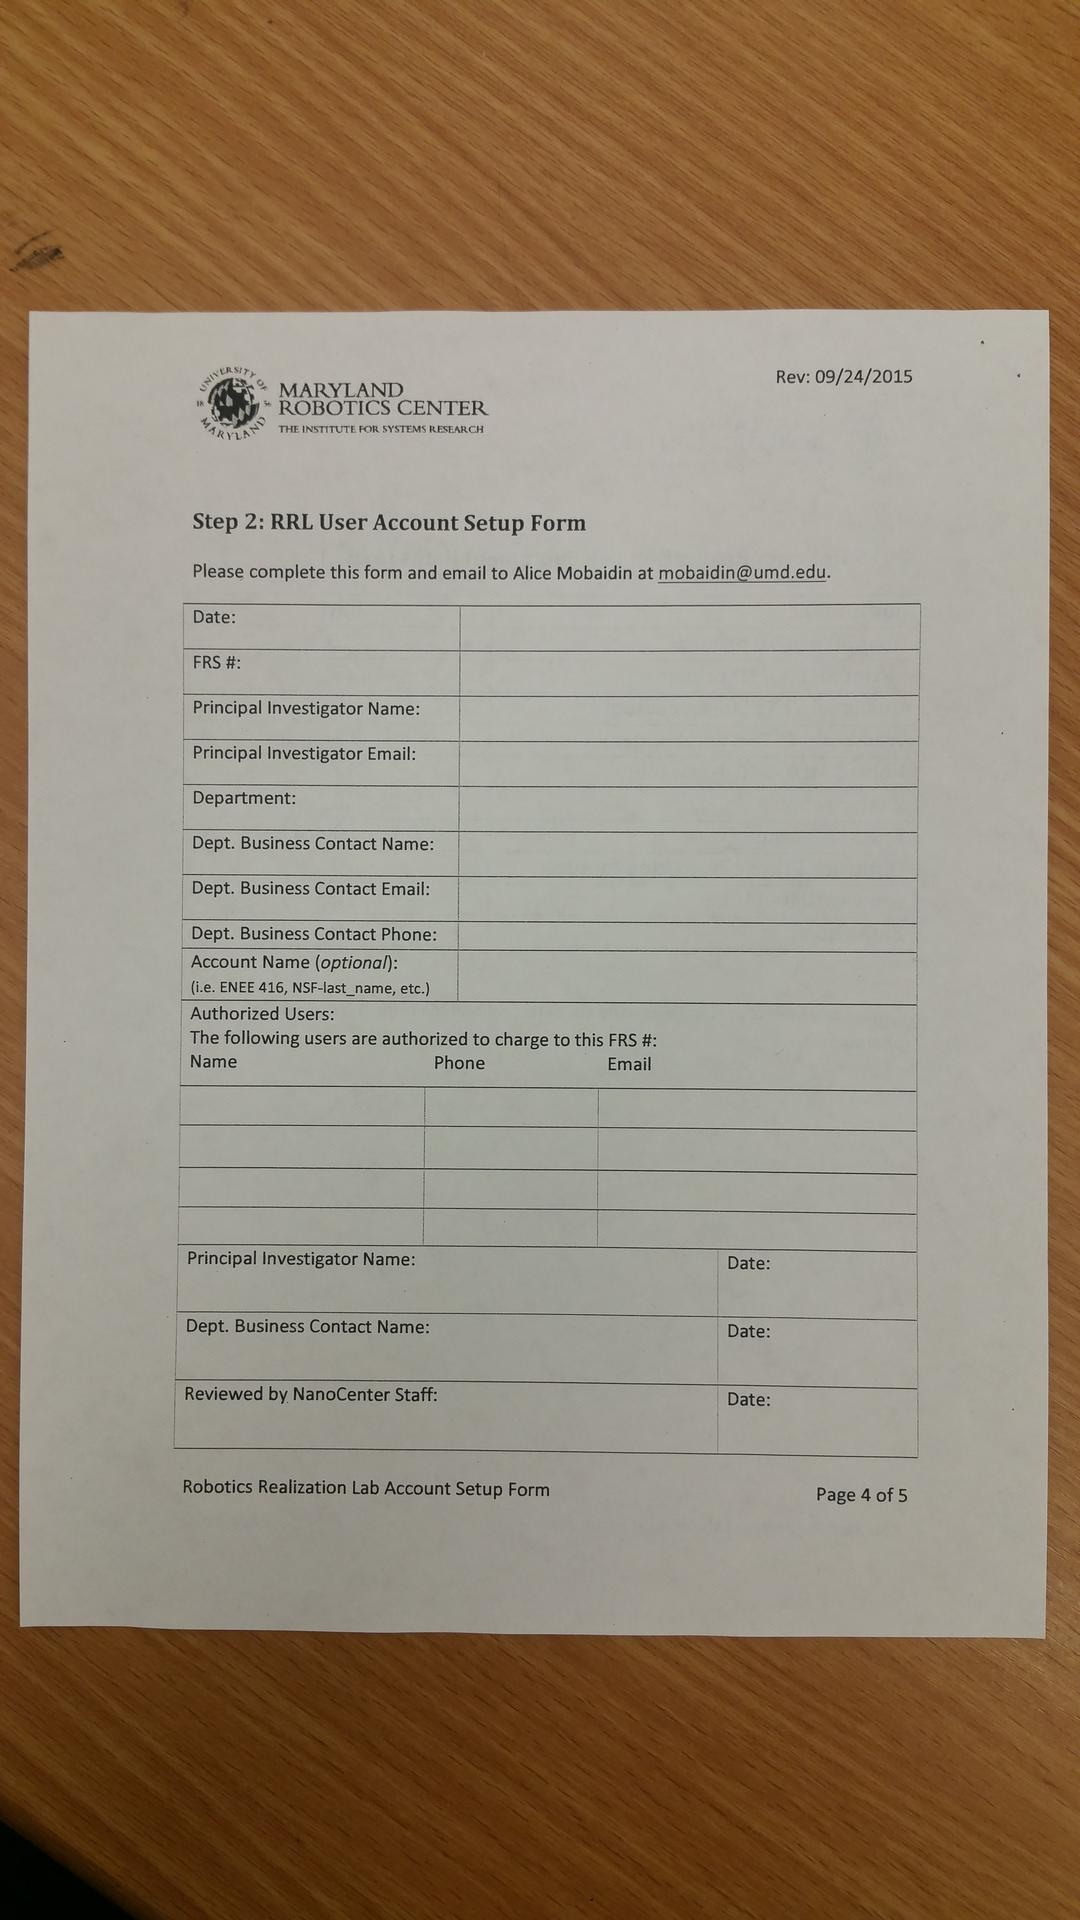
\includegraphics[height=18cm ]{Figures/resized_input}
	%	\decoRule
	\caption[Reference Image]{Reference Image.}
	\label{fig:ReferenceImage}
\end{figure}

\pagebreak
All the techniques involved in extracting the document/sheet from the given image are briefly explained below. \\

\subsection{Image Enhancement}

The input RGB image is resized to be below 640 X 480 pixels, if the image size is greater than that. Then the resized image is converted to grayscale by doing weighted addition of R, G and B components and normalizing them to fit 0 to 255 scale. Then the image is sharpened in-order to boost its edges. The edges can be \keyword{sharpened} by adding a portion of the high pass filtered image to the original image. In order to smoothen out any noise in the image, \keyword{bilateral filter} (\cite{Reference17}) is used. The bilinear filter implemented as a part of this project uses a kernel size of 5 with gaussian weight of 25 and range weight of 15 . The bilateral filter basically does gaussian filtering everywhere in the image except at the edges. \\ \\
 The resulting enhanced image is shown below. \\


\begin{figure}[th]
	\centering
	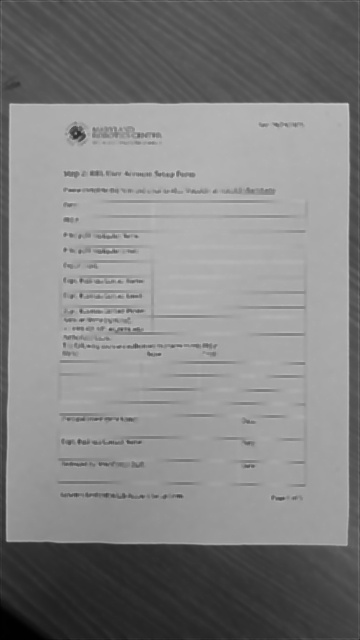
\includegraphics[height=15cm ]{Figures/image_enhancement}
%	\decoRule
	\caption[Image Enhancement]{Image Enhancement.}
	\label{fig:ImageEnhancement}
\end{figure}

\subsection{Canny Edge Detection}

The edges from the enhanced image can be extracted using the \keyword{Canny Edge Detection} method (\cite{Reference7} ). 
\\
\\
The canny edge detection algorithm proceeds as shown in the flow chart below.
\\
\\
	\begin{center}
	\begin{figure}[hbt]
	\centering
	\begin{tikzpicture}
	\matrix (m)[matrix of nodes, column  sep=0cm,row  sep=8mm, align=center, nodes={rectangle,draw, anchor=center} ]{
		|[block]| {Start}              &  \\
		|[block]| {Input Image}              &  \\
		|[block]| { Gaussian Blur }               &                                            \\
		|[block]| {Sobel Filter}          &             \\
		|[block]| {Non Maximum Suppression}    &                                             \\
		|[block]| {Double Thresholding}    &         \\
		|[block]| {Hysterisis}    &                   \\
		|[block]| {Edges}        &             \\
		|[block]| {Stop}        &             \\
	};
	\path [>=latex,->] (m-1-1) edge (m-2-1);
	\path [>=latex,->] (m-2-1) edge (m-3-1);
	\path [>=latex,->] (m-3-1) edge (m-4-1);
	\path [>=latex,->] (m-4-1) edge (m-5-1);
	\path [>=latex,->] (m-5-1) edge (m-6-1);
	\path [>=latex,->] (m-6-1) edge (m-7-1);
	\path [>=latex,->] (m-7-1) edge (m-8-1);
	\path [>=latex,->] (m-8-1) edge (m-9-1);

	\end{tikzpicture}

	\caption{Flow Chart for Canny Edge Detection}
`   \label{fig:CannyEdgeDetectionFlowChart}

\end{figure}
\end{center}


This is a multi-step edge detection algorithm that typically uses and optimizes other edge detection operators such as Prewitt, Robert and Sobel. First the input image is smoothened with a \keyword{Gaussian Filter}. Then an edge detection operator like \keyword{Sobel Filter} is applied to the image and the intensity gradient and direction is computed. Based on the gradient and its direction, \keyword{non maximum suppression} is applied to make the edges thinner. Strong and weak edges from the resulting image are identified by \keyword{double thresholding} it. The weak edges are then tracked to see if its connected to other strong edges, in which case the weak edge will now be considered as strong edge or will be eliminated otherwise. This process is called \keyword{hysterisis}.

\pagebreak

The result of canny edge detection on the previously enhance image is shown below. \\ \\

\begin{figure}[th]
	\centering
	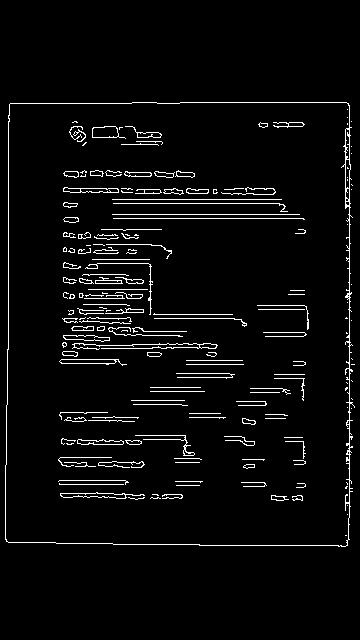
\includegraphics[height=18cm ]{Figures/canny_edge_detection}
	%	\decoRule
	\caption[Canny Edge Detection]{Canny Edge Detection.}
	\label{fig:CannyEdgeDetection}
\end{figure}
\pagebreak
\subsection{Morphological Operations}

The edges extracted from the enhanced image can sometimes have some discontinuities and minute holes that might need to be eliminated for further processing to work. In order to do that, a variety of morphological operations,namely \keyword{Erosion} and \keyword{Dilation}, are used. Dilation replaces the pixel in an image with the pixel that has the highest value. Hence, this operation thickens the white edges. Erosion on the other hand replaces the pixel in an image with the pixel that has the lowest value. Thus, this operation thins the white edges. A combination of these two operations can be used to do morphological opening and closing. The edges are first dilated and then eroded in order to close the discontinuities. This combination is referred to as \keyword{ morphological closing}. Then the edges are eroded and dilated in order to make the edges thinner. This combination is referred to as \keyword{morphological opening}.
\\
\\
The result of morphological closing and opening on the extracted edges are shown below.\\ 

\begin{figure}[th]
	\centering
	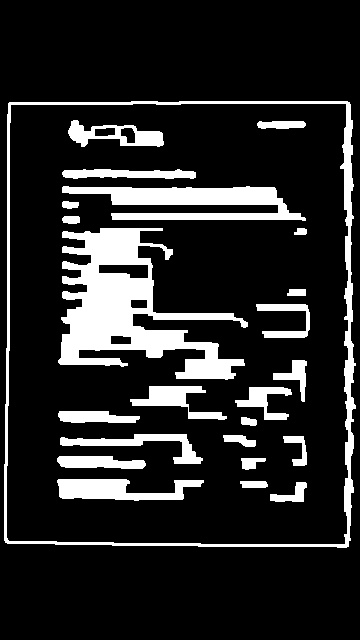
\includegraphics[height=16cm ]{Figures/morphological_operation}
	%	\decoRule
	\caption[Morphological Operations]{Morphological Operations.}
	\label{fig:MorphologicalOperations}
\end{figure}

\pagebreak

\subsection{Contour Detection}

The image computed previously contains a lot of \keyword{contours}. The contours from this image are extracted using OpenCV's (\cite{Reference1}) \keyword{'findContour'} function . Contours are estimated by using the \keyword{Boundary Following Algorithm for Topological Analysis}, proposed by \cite{Reference4}. The largest convex contour, with 4 vertices, is found and the pixels inside this contour is assumed to contain the document that has to be scanned .
\\
\\
The estimated contour is overlaid on the original image and shown below.\\ 

\begin{figure}[th]
	\centering
	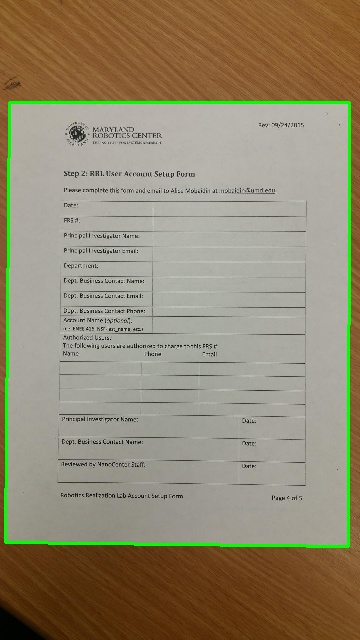
\includegraphics[height=16cm ]{Figures/contour_detection}
	%	\decoRule
	\caption[Contour Detection]{Contour Detection.}
	\label{fig:ContourDetection}
\end{figure}

\pagebreak

\subsection{Harris Corner Detection}

The contour estimated above basically has 4 corners. In order to compute them \keyword{Harris Corner Detection} (\cite{Reference6}) is used. 
\\
\\
The Harris Corner Detection algorithm proceeds as shown in the flow chart below.
\\
\\
\begin{center}
	\begin{figure}[hbt]
		\centering
		\begin{tikzpicture}
		\matrix (m)[matrix of nodes, column  sep=0cm,row  sep=8mm, align=center, nodes={rectangle,draw, anchor=center} ]{
			|[block]| {Start}              &  \\
			|[block]| {Estimated Contour}              &  \\
			|[block]| {Sobel Filter}          &             \\
			|[block]| {Compute Harris Matrix 
					   \[
					   M =\Sigma_{x,y}w(x,y)
					   \begin{bmatrix}
					   I_{x}^{2} & I_{x}I_{y}  \\
					   I_{x}I_{y} & I_{y}^{2} 
					   \end{bmatrix}
					   \]}          &             \\
			|[block]| {Compute Harris Response
					$ R= |M| -k.Trace(M^{2}) $}    &                                             \\
			|[block]| {Adaptive Thresholding}    &         \\
			|[block]| {Non Maxima Suppression}        &             \\
			|[block]| {Corners}        &             \\
			|[block]| {Stop}        &             \\
		};
		\path [>=latex,->] (m-1-1) edge (m-2-1);
		\path [>=latex,->] (m-2-1) edge (m-3-1);
		\path [>=latex,->] (m-3-1) edge (m-4-1);
		\path [>=latex,->] (m-4-1) edge (m-5-1);
		\path [>=latex,->] (m-5-1) edge (m-6-1);
		\path [>=latex,->] (m-6-1) edge (m-7-1);
		\path [>=latex,->] (m-7-1) edge (m-8-1);
		\path [>=latex,->] (m-8-1) edge (m-9-1);
		
		\end{tikzpicture}
		
		\caption{Flow Chart for Harris Corner Detection}
		`   \label{fig:HarrisCornerDetectionFlowChart}
		
	\end{figure}
\end{center}

Harris Corner Detection method estimates the location of corners based on the gradients at each pixel. It fundamentally relies on the property that corners have large gradients in both x and y direction. The algorithm proceeds by computing the x and y gradients of the image using operators like Sobel. Based on these gradients, the Harris Matrix is computed. Then the Harris Response is obtained from the Harris Matrix M where k's best estimate by Harris was found to be 0.04. The response image is adaptively thresholded in order to obtain the corners. There might be a lot of estimated corners very close to each other , these group of corners are replaced by just one corner by doing non-maxima suppression. 

\pagebreak

The result of harris corner detection on the estimated contour is overlaid on the original image shown below \\ \\

\begin{figure}[th]
	\centering
	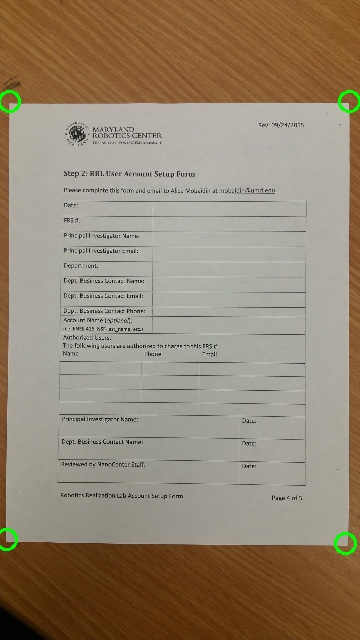
\includegraphics[height=18cm ]{Figures/corner_detection}
	%	\decoRule
	\caption[Corner Detection]{Corner Detection.}
	\label{fig:CornerDetection}
\end{figure}

\pagebreak

\subsection{Perspective Transform and Warping}

The four corners obtained above are ordered in the clockwise manner. The width and height of the contour are approximated based on the location of these corners and then a reference rectangle is constructed based on this. 
\\
\\
The \keyword{perspective transform} (\cite{Reference16}) between the corners of the contour and the corners of the reference rectangle can be computed to warp the image as shown below. \\

\begin{center}
		\centering
	\begin{figure}[hbt]
		\centering
		\begin{tikzpicture}
		\matrix (m)[matrix of nodes, column  sep=1cm,row  sep=7mm, align=center, nodes={rectangle,draw, anchor=center} ]{
			|[block]| {Start}              &  \\
			|[block]| {Corners}              &  \\
			|[block]| {Order Clockwise}          &             \\
			|[block]| {Solve the following for 4 corners 
				\[
				\begin{bmatrix}
				x_{1} & x_{2} & x_{3}  \\
				y_{1} & y_{2} & y_{3} \\
				1 & 1 & 1
				\end{bmatrix}.\begin{bmatrix}
				\lambda  \\
				\mu \\
				\tau
				\end{bmatrix} = \begin{bmatrix}
				x_{4}  \\
				y_{4} \\
				1
				\end{bmatrix}
				\]}          &             \\
			|[block]| {Scale columns by \\ computed coefficients
								\[ A = 
				\begin{bmatrix}
			\lambda.x_{1} & \mu .x_{2} & \tau .x_{3}  \\
			\lambda	.y_{1} & \mu .y_{2} & \tau .y_{3} \\
			\lambda & \mu & \tau
				\end{bmatrix}\]}    &                    \\
			|[block]| {Repeat previous 2 steps for reference rectangle to get B}    &  |[block]| {Stop}                                 \\
			|[block]| {Compute Perspective Transform\\ $ C = B.A^{-1}  $}        &     	|[block]| {Do Bilinear Interpolation}            \\
			|[block]| { Get homogeneous co-ordinates of transformed points\[ \begin{bmatrix}
				x^{'}  \\
				y^{'} \\
				z^{'}
				\end{bmatrix} = C. \begin{bmatrix}
				x  \\
				y \\
				z
				\end{bmatrix}
				\]}        &            
			|[block]| {Warp Image by normalizing homogeneous co-ordinates \\ $ x^{''} = \dfrac{x^{'}}{z^{'}} \ ,\  y^{''} = \dfrac{y^{'}}{z^{'}} $}        &             \\
		};
		\path [>=latex,->] (m-1-1) edge (m-2-1);
		\path [>=latex,->] (m-2-1) edge (m-3-1);
		\path [>=latex,->] (m-3-1) edge (m-4-1);
		\path [>=latex,->] (m-4-1) edge (m-5-1);
		\path [>=latex,->] (m-5-1) edge (m-6-1);
		\path [>=latex,->] (m-6-1) edge (m-7-1);
		\path [>=latex,->] (m-7-1) edge (m-8-1);
		\path [>=latex,->] (m-8-1) edge (m-8-2);
		\path [>=latex,->] (m-8-2) edge (m-7-2);
		\path [>=latex,->] (m-7-2) edge (m-6-2);
		\end{tikzpicture}
		\caption{Flow Chart for Computing Perspective Transform}
		`   \label{fig:PerspectiveTransformComputation}
	\end{figure}
\end{center}

\pagebreak

The result of \keyword{warping} the image using the computed perspective transform and doing \keyword{bilinear interpolation} is shown below\\ \\

\begin{figure}[th]
	\centering
	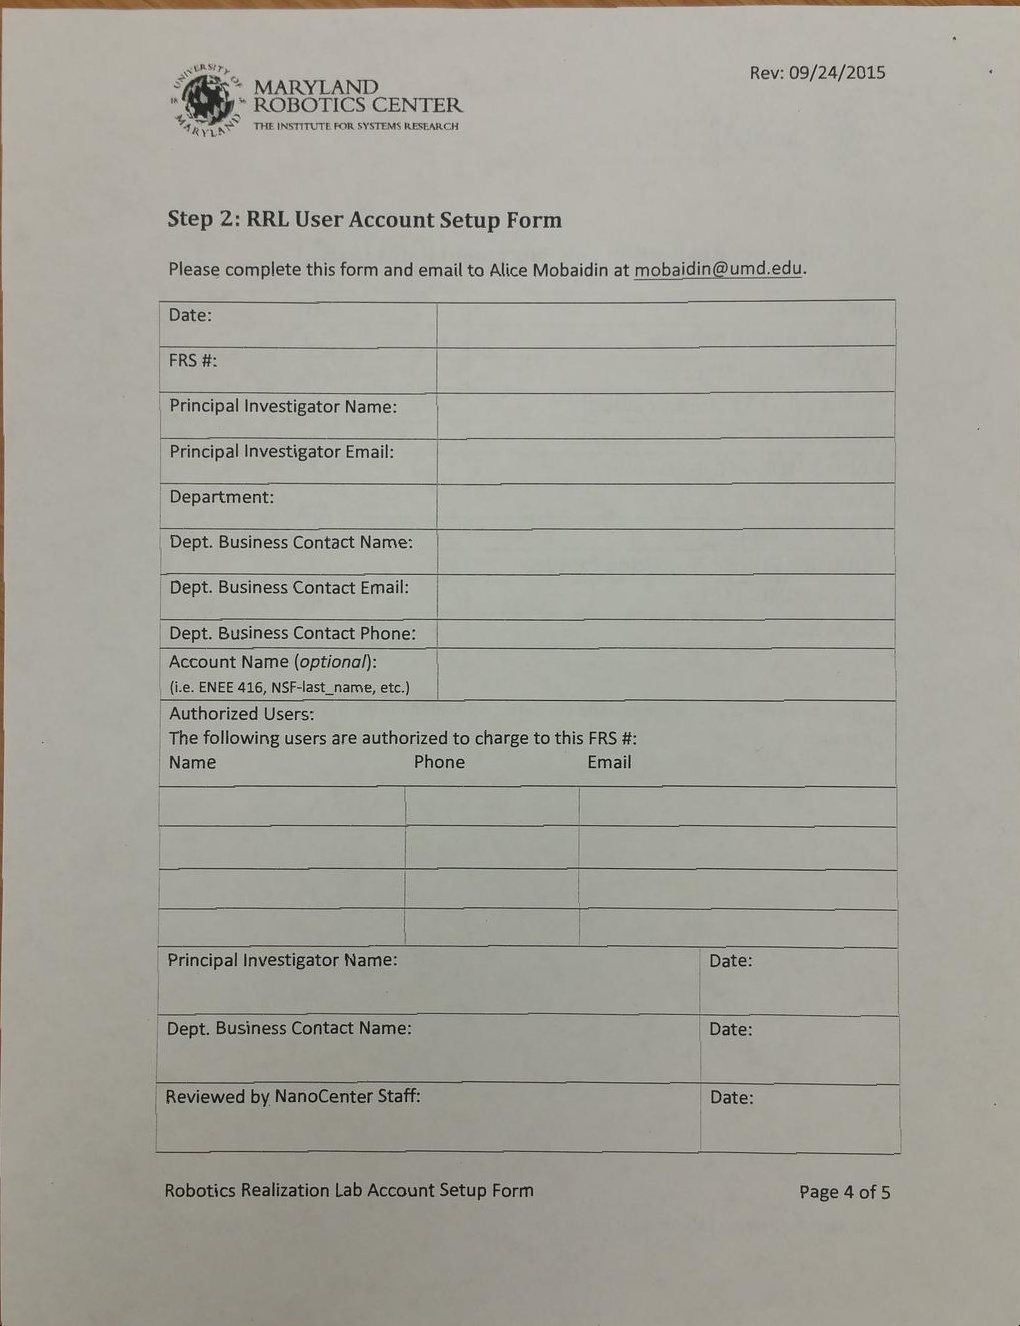
\includegraphics[height=18cm ]{Figures/warped_image}
	%	\decoRule
	\caption[Warped Reference Image]{Warped Reference image.}
	\label{fig:WarpedReferenceImage}
\end{figure}

\pagebreak

\subsection{Adaptive Thresholding}

The warped RGB image can be converted to binary Black/White format, suitable for printing/registration purposes, by doing \keyword{Adaptive Thresholding} (\cite{Reference10}) . This is a data dependent thresholding technique. It's fundamental principle is that the region of interest can be segmented out by using the blurred version of an image minus a constant as the threshold. Different types of filters like Mean filters, Gaussian filter , Median filter can be used to blur the image. Here the Gaussian Minus C algorithm is used. C was experimentally determined to be 5. This would be really useful for \keyword{text segmentation} (\cite{Reference14}) \. \\ \\ The adaptively thresholded reference image is shown below. \\

\begin{figure}[th]
	\centering
	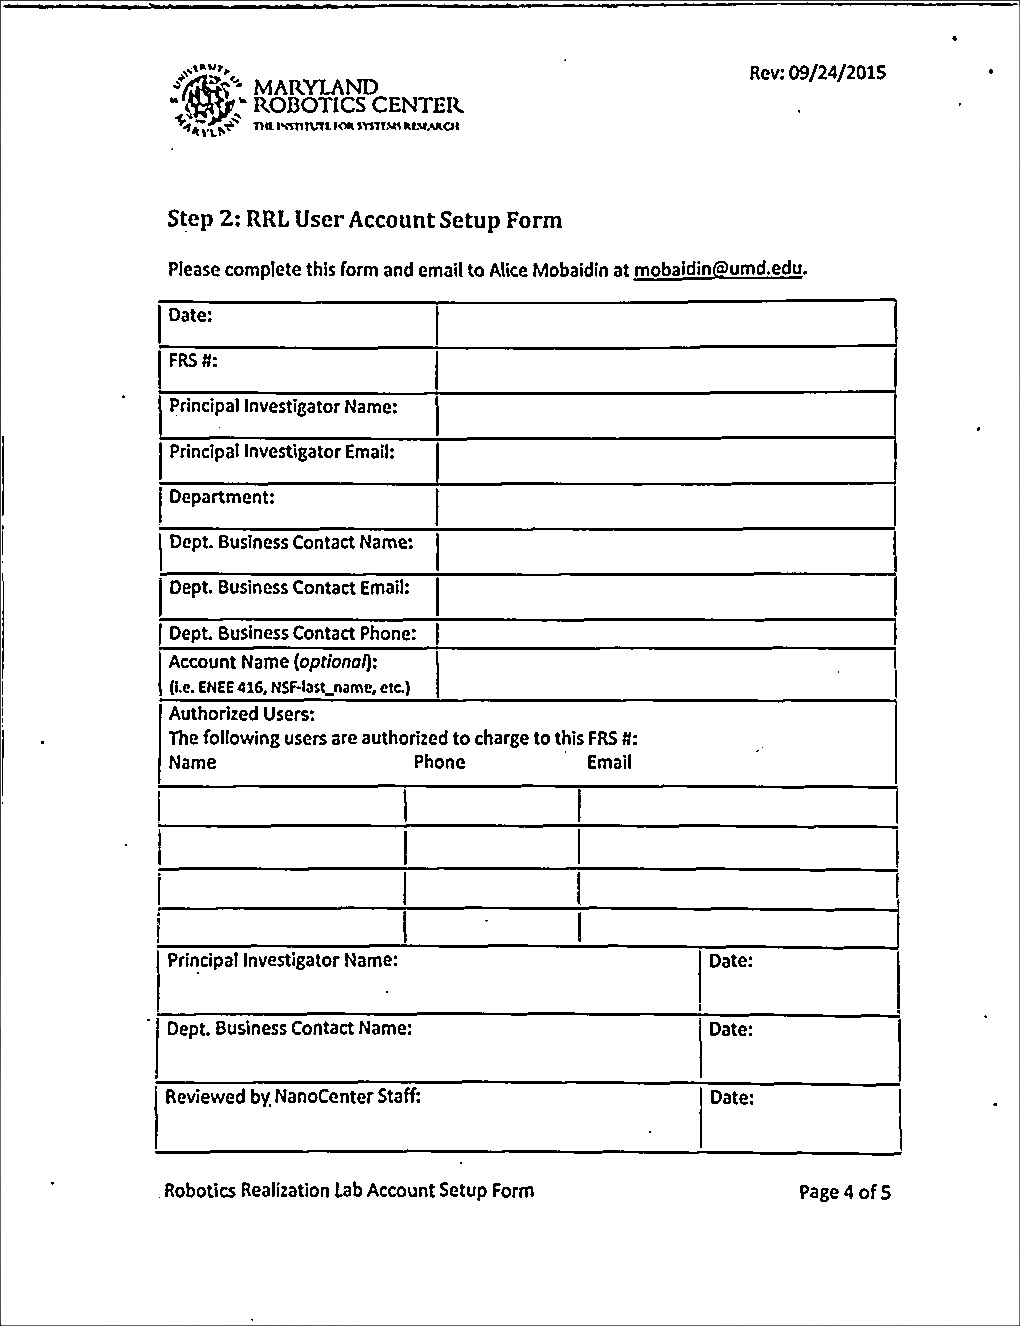
\includegraphics[height=17cm ]{Figures/adaptive_thresholding}
	%	\decoRule
	\caption[AdaptiveThresholding]{Adaptive Thresholding.}
	\label{fig:AdaptiveThresholding}
\end{figure}




%----------------------------------------------------------------------------------------


 
% Chapter 2
% \ref{Chapter1}
%\begin{figure}
\chapter{Image Registration} % Main chapter title
\label{Chapter3} % For referencing the chapter elsewhere, use
%----------------------------------------------------------------------------------------

\section{Flow Chart}
\nopagebreak
% Define block styles
\tikzset{
	desicion/.style={
		diamond,
		draw,
		text width=6em,
		text badly centered,
		inner sep=0pt
	},
	block/.style={
		rectangle,
		draw,
		text width=15em,
		text centered,
		rounded corners
	},
	cloud/.style={
		draw,
		ellipse,
		minimum height=1em
	},
	descr/.style={
		fill=white,
		inner sep=2.5pt
	},
	connector/.style={
		-latex,
		font=\scriptsize
	},
	rectangle connector/.style={
		connector,
		to path={(\tikztostart) -- ++(#1,0pt) \tikztonodes |- (\tikztotarget) },
		pos=0.5
	},
	rectangle connector/.default=-2cm,
	straight connector/.style={
		connector,
		to path=--(\tikztotarget) \tikztonodes
	}
}
\begin{center}
	\begin{figure}[hbt]
		\centering
	\begin{tikzpicture}
\matrix (m)[matrix of nodes, column  sep=2cm,row  sep=8mm, align=center, nodes={rectangle,draw, anchor=center} ]{
	|[block]| {Start}              &  \\
	|[block]| { Extract the reference document to be registered from the image}               &                                            \\
	|[block]| {Compute ORB Features in the reference document \\ and scanned image}          &  \\
	|[block]| {Filter out atleast 500 matching features based on Ratio Test and Symmetry Test}    &                                             \\
	|[block]| {Find the 4 best matching features using RANSAC}    &                                          \\
	|[block]| {Compute the perspective transform that associates 4 best matching features in the reference document \\ and scanned image}    &    |[block]| {Stop}                                          \\
	|[block]| {Warp the scanned image to align it with the reference document and do bilinear interpolation}        &       |[block]| {Adaptive Thresholding}                                      \\
	|[block]| {Extract filled text from the scanned document by doing\\ background subtraction}    &   |[block]| { Add the extracted text to the reference document }                                         \\
};
\path [>=latex,->] (m-1-1) edge (m-2-1);
\path [>=latex,->] (m-2-1) edge (m-3-1);
\path [>=latex,->] (m-3-1) edge  (m-4-1);
%\draw [>=latex,->] (m-3-2) |- (m-4-1);
\path [>=latex,->] (m-4-1) edge (m-5-1);
\path [>=latex,->] (m-5-1) edge (m-6-1);
\path [>=latex,->] (m-6-1) edge (m-7-1);
\path [>=latex,->] (m-7-1) edge (m-8-1);
\path [>=latex,->] (m-8-1) edge (m-8-2);
\path [>=latex,->] (m-8-2) edge (m-7-2);
\path [>=latex,->] (m-7-2) edge (m-6-2);

\end{tikzpicture}
    \caption{Flow Chart for Image Registration}
\label{fig:ImageRegistrationFlowChart}
\end{figure}
\end{center}
%\caption[Document Extraction]{Flowchart for Document Extraction.}


%\end{figure}

\section{Image Registration Techniques}

Consider the image shown below from which the text is to be extracted and overlaid on top of the reference document. 
\\ \\

\begin{figure}[th]
	\centering
	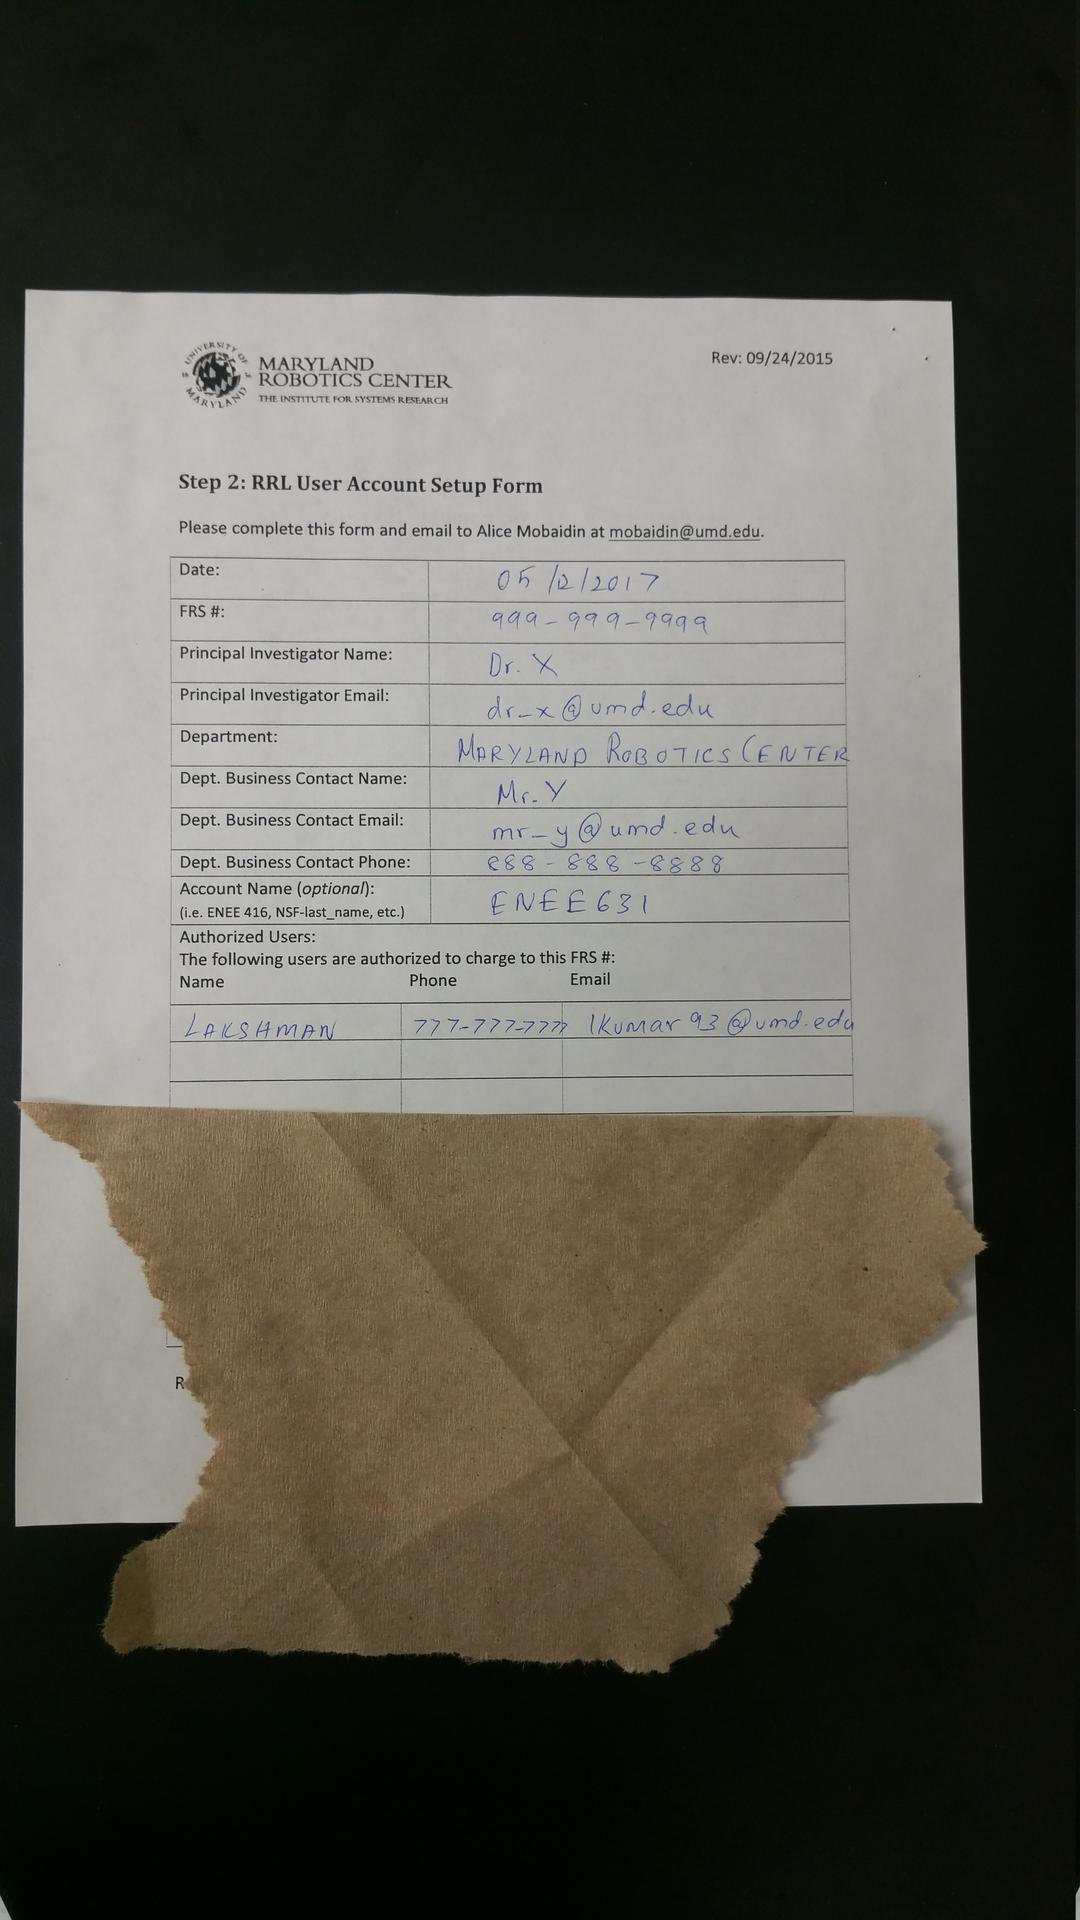
\includegraphics[height=18cm ]{Figures/scanned_image}
	%	\decoRule
	\caption[ScannedImage]{Scanned Image}
	\label{fig:ScannedImage}
\end{figure}

\pagebreak
All the techniques involved in extracting filled text from the scanned image and overlaying it on top of the reference document are briefly explained below. \\

\subsection{Image Alignment}

\keyword{ORB feature detector} (\cite{Reference3}) is an effective replacement to \keyword{SIFT} (\cite{Reference8}) and \keyword{SURF} (\cite{Reference9}) in terms of computation cost. It is basically a rotational invariant version of \keyword{FAST} keypoint detector (\cite{Reference12}) and \keyword{BRIEF} keypoint descriptor (\cite{Reference13}).ORB features are computed in both the reference document and the scanned image using \keyword{OpenCV's feature detection API} . These features are then matched between the reference document and scanned image using \keyword{Brute Force Hamming} technique with \keyword{KNN} (\cite{Reference15}), the rest of features are weeded out. These features are further filtered on whether they satisfy the ratio test and the symmetry test. As per the ratio test, matching features, for which the ratio of the nearest neighbor distance to the second nearest neighbor distance is greater than 0.8, are rejected to extract good matches. As per the symmetry test, good matches that correspond from reference image to scanned image and vice versa should be the same or else they are eliminated. Hence better matches can be extracted. It is also made sure that there are at least 500 matches that satisfy both tests between the two images. Hence the number of ORB features are iteratively increased until this constraint is satisfied. \\ \\
The better matches computed in both the reference document and scanned document are shown below. \\ \\ 
\begin{figure}[th]
	\centering
	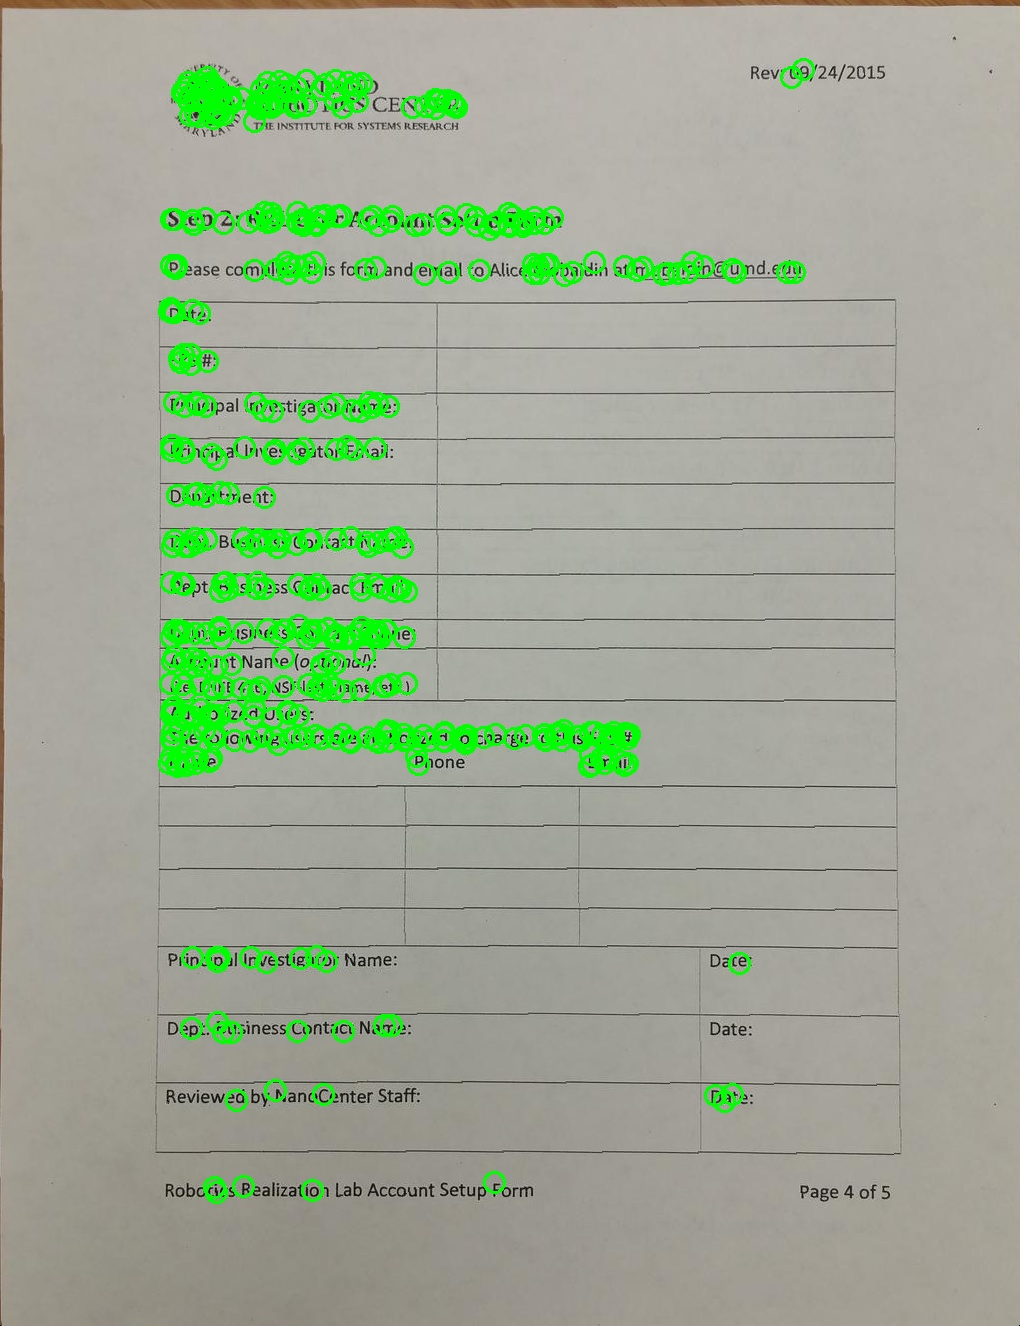
\includegraphics[height=11cm ]{Figures/orb_reference_image}
	%	\decoRule
	\caption[Matching Orb Features in Reference Document]{Matching Orb Features in Reference Document.}
	\label{fig:ReferenceDocumentORBFeatures}
\end{figure}

\pagebreak
\begin{figure}[th]
	\centering
	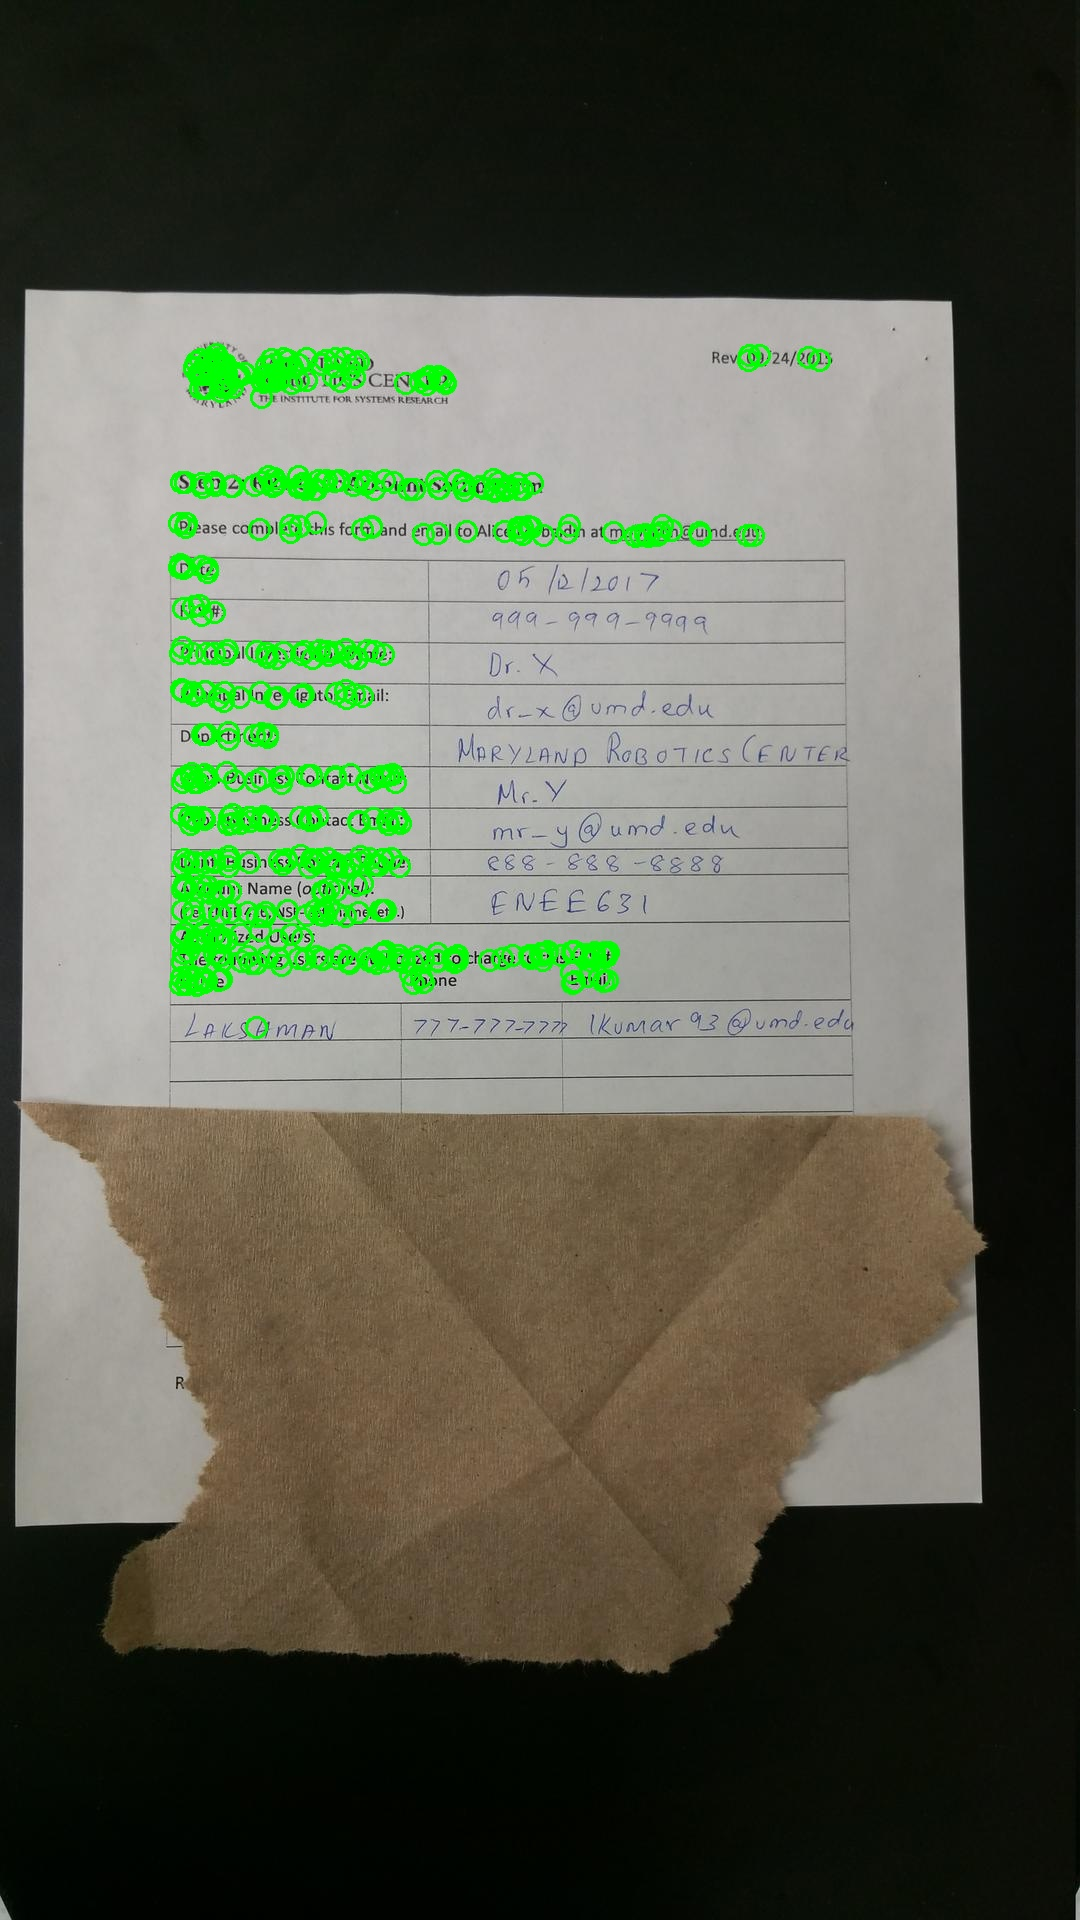
\includegraphics[height=18cm ]{Figures/orb_scanned_image}
	%	\decoRule
	\caption[Matching Orb Features in Scanned Image]{Matching Orb Features in Scanned image.}
	\label{fig:ScannedImageORBFeatures}
\end{figure}

\pagebreak

 In order to obtain the perspective transform linking the two images, 4 matches are required. The best 4 matches can be computed using \keyword{RANSAC} (\cite{Reference11}) . RANSAC is an iterative method to remove outliers. RANSAC initially randomly chooses 4 non-identical matches from the set of better matches and computes the perspective transform between these 4 matches of both the images. The matching features in the scanned image are then warped by the computed perspective transform and checked to see if the euclidean distance between the warped feature and the matching feature in the reference document is less than a certain threshold, which was experimentally determined to be 0.175 . If so, that particular feature is considered to be matching. This process is repeated for all the better matches and for a certain number of iterations, in this case, 50000. The perspective transform that has the most number of matching points is considered to be the best and this is used to warp the scanned image to align with the reference document. \\ \\
 The best four matches are shown below \\ \\ 
 
\begin{figure}[th]
	\centering
	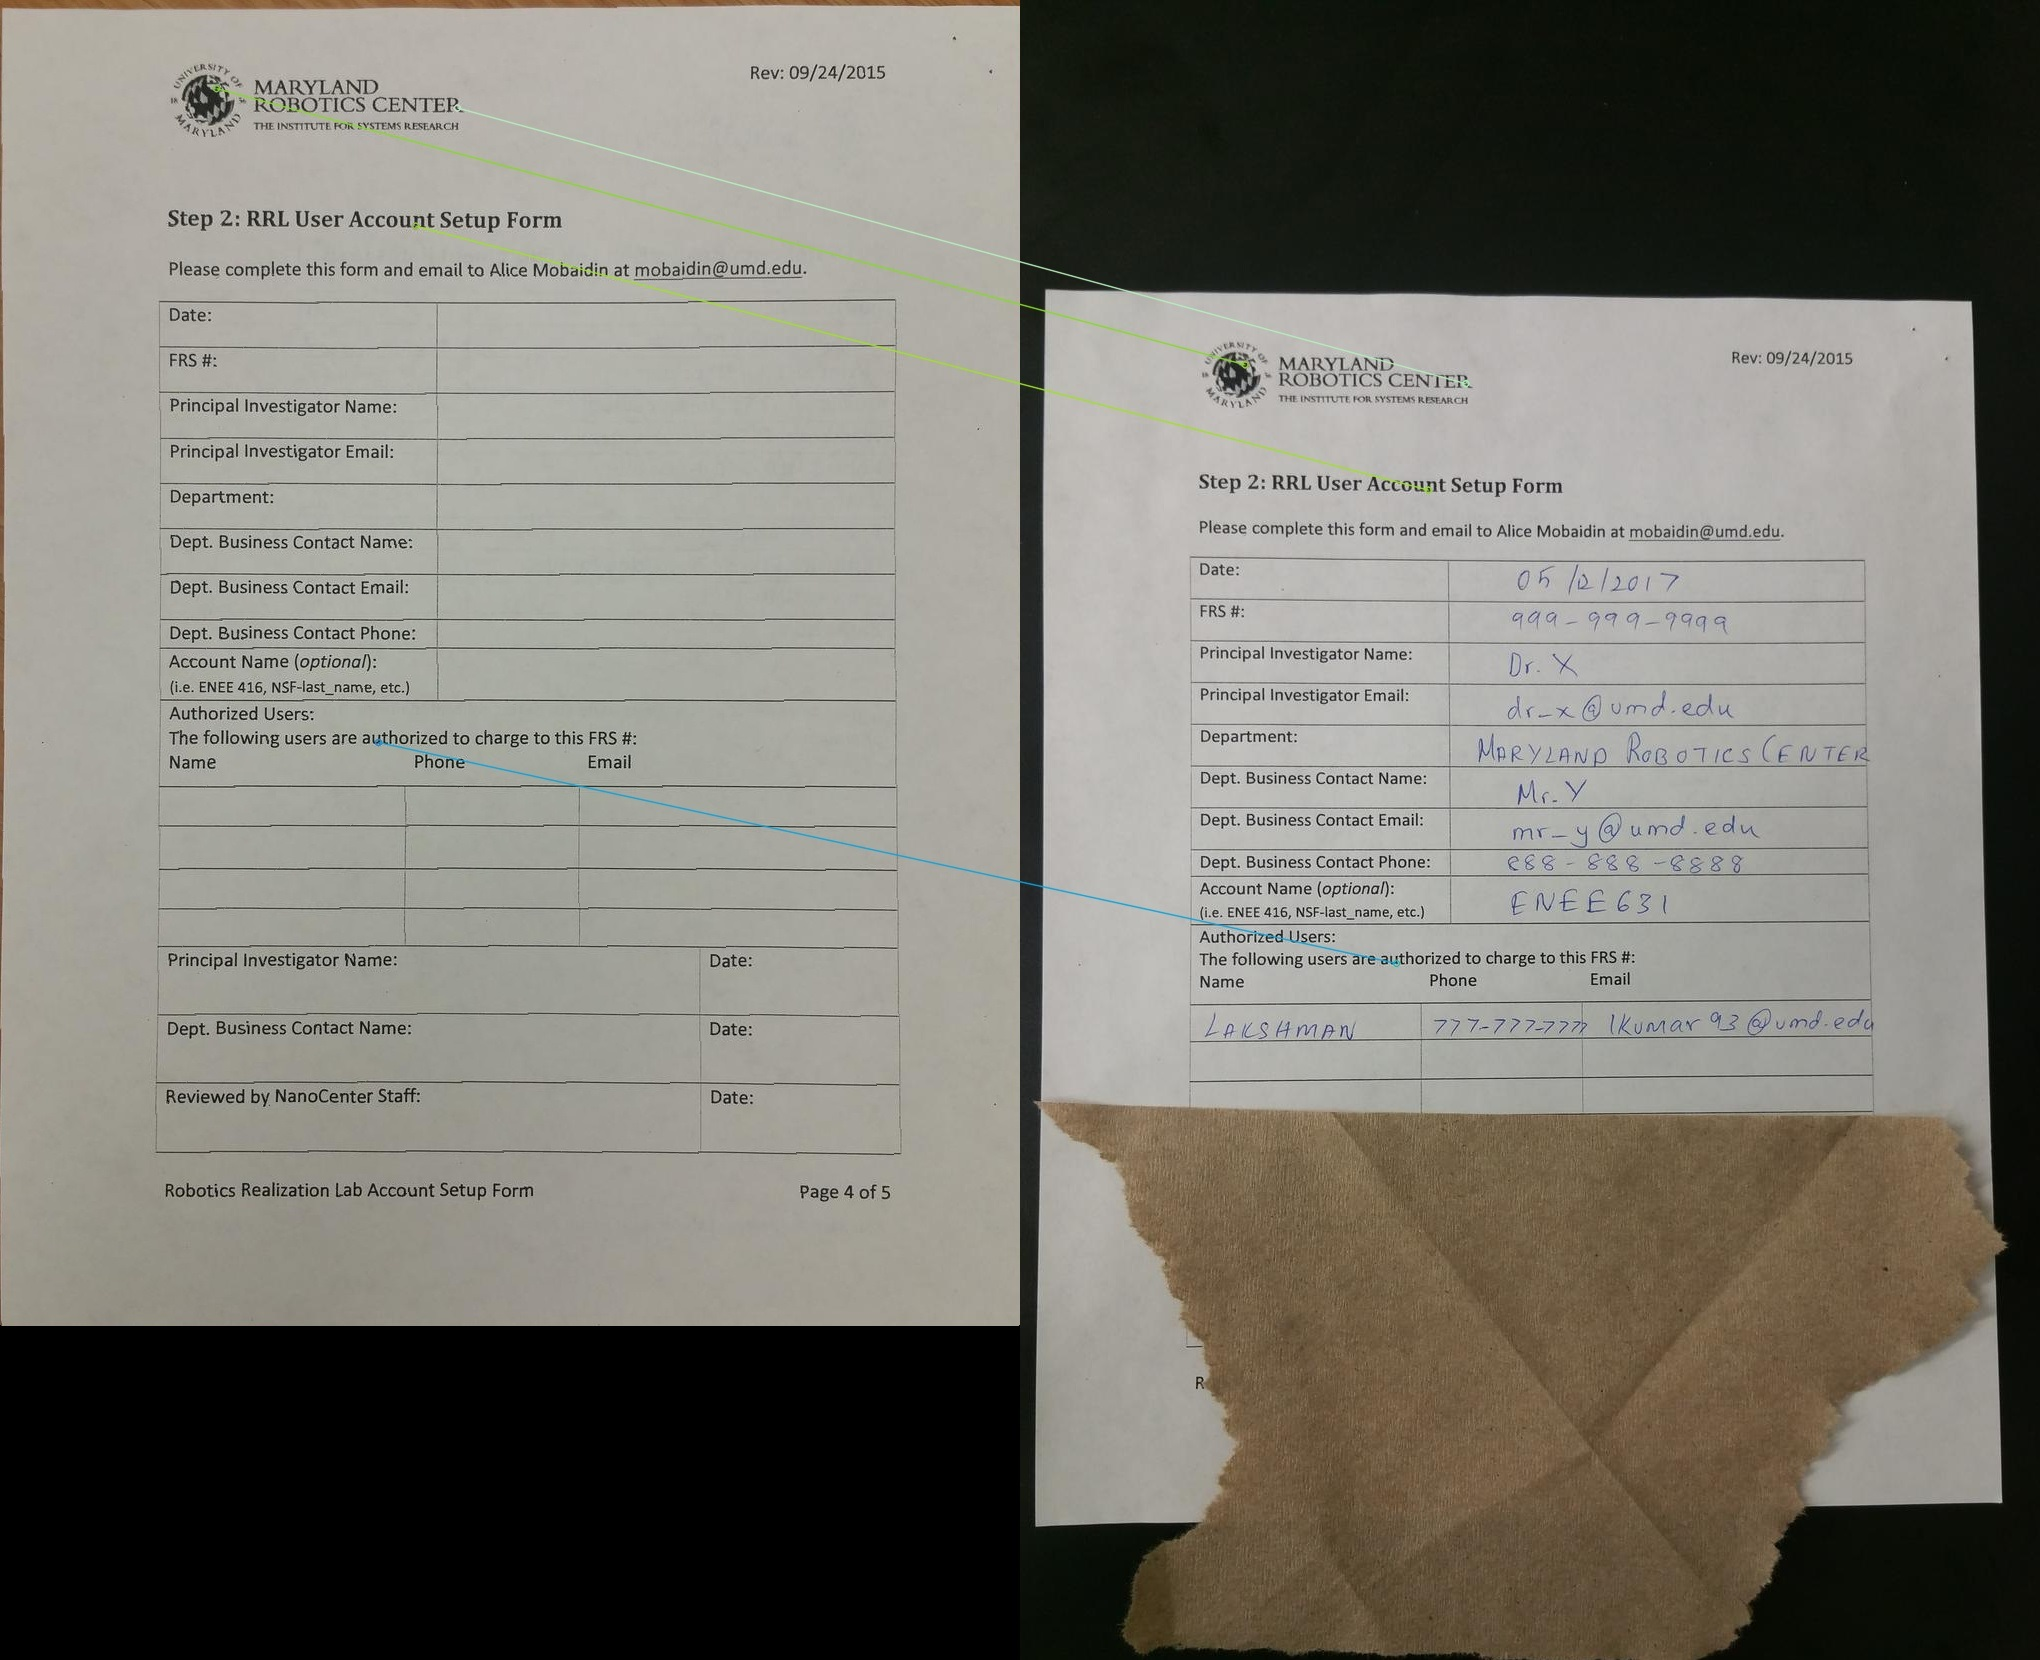
\includegraphics[height=13cm ]{Figures/best_four_matches_ransac}
%	\decoRule
	\caption[Best Matches]{Best Matches.}
	\label{fig:BestMatches}
\end{figure}
\pagebreak

 The aligned version of scanned document is shown below \\ \\ 
 
\begin{figure}[th]
	\centering
	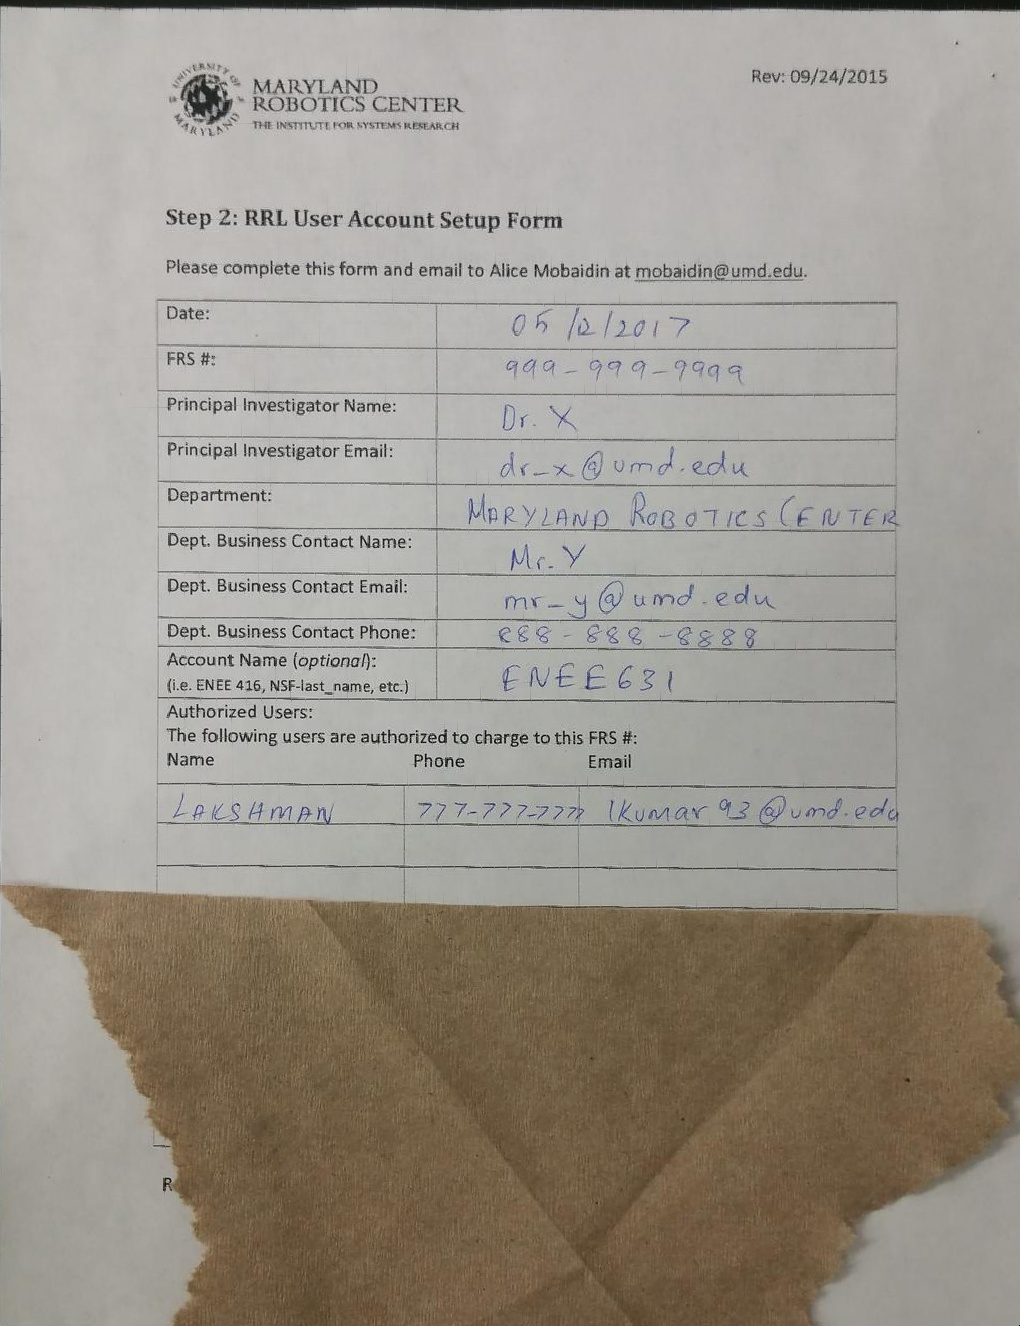
\includegraphics[height=18cm ]{Figures/warped_scanned_image}
	%	\decoRule
	\caption[Warped Scanned Document]{Warped Scanned Document.}
	\label{fig:WarpedFilledDocument}
\end{figure}
\pagebreak


\subsection{Background Subtraction}

Background Subtraction is done in order to extract the filled text from scanned document. In order to do that , both the reference document and the scanned document are converted to grayscale and then sharpened to boost its edges. The sharpened images are then further adaptively thresholded to convert them to a binary image.
\\
\\
The adaptively thresholded images are shown below.
\\
\\
\begin{figure}[th]
	\centering
	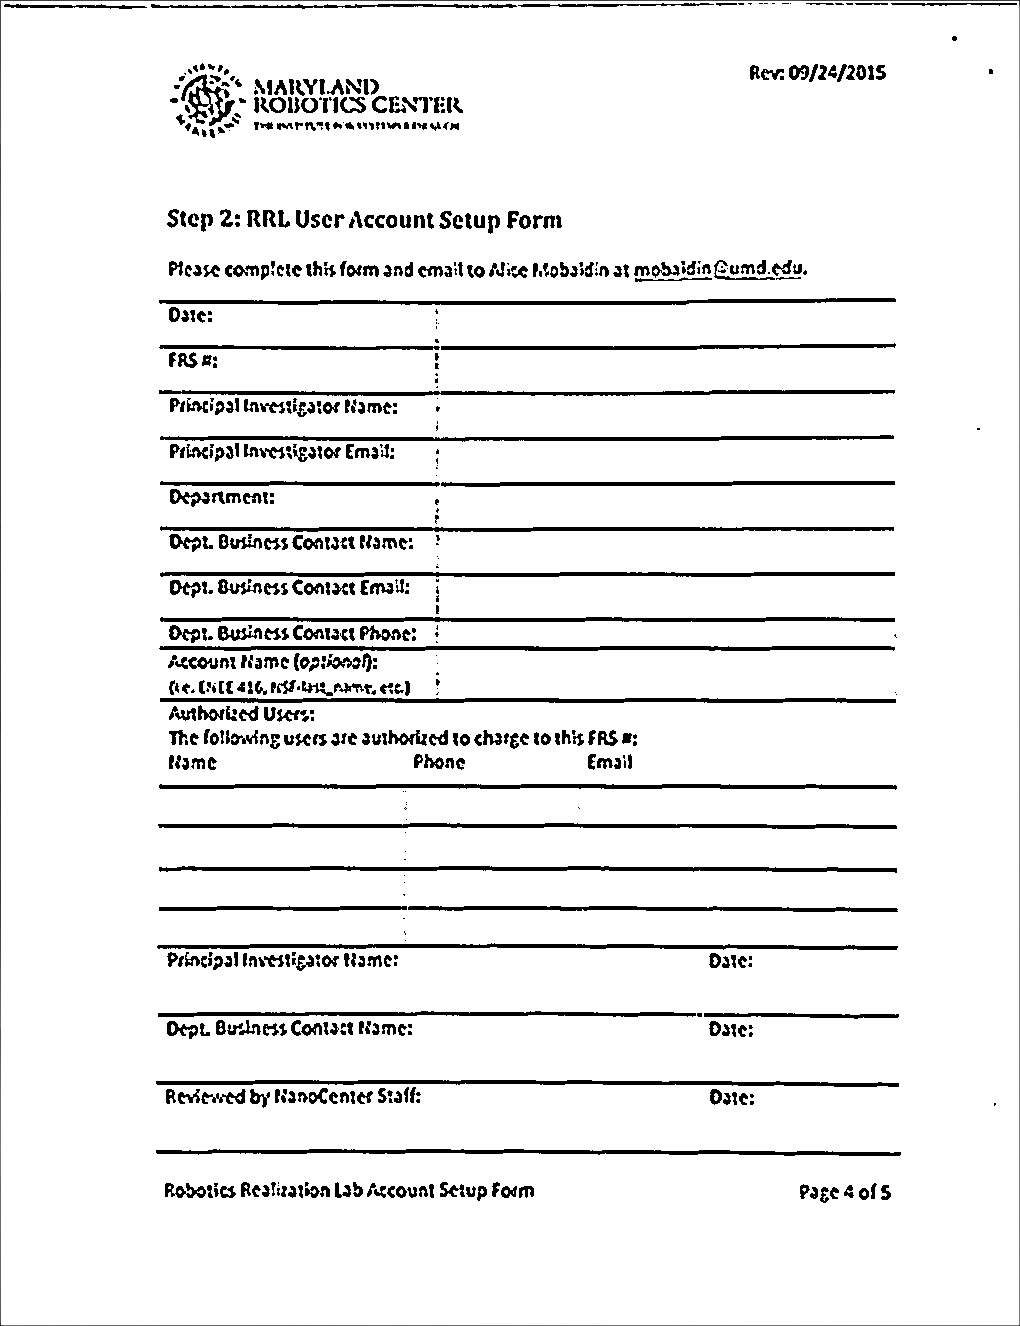
\includegraphics[height=15cm ]{Figures/thresholded_reference_image}
	%	\decoRule
	\caption[Thresholded Reference Document]{Thresholded Reference Document.}
	\label{fig:ThresholdedReferenceDocument}
\end{figure}	

\pagebreak

\begin{figure}[th]
	\centering
	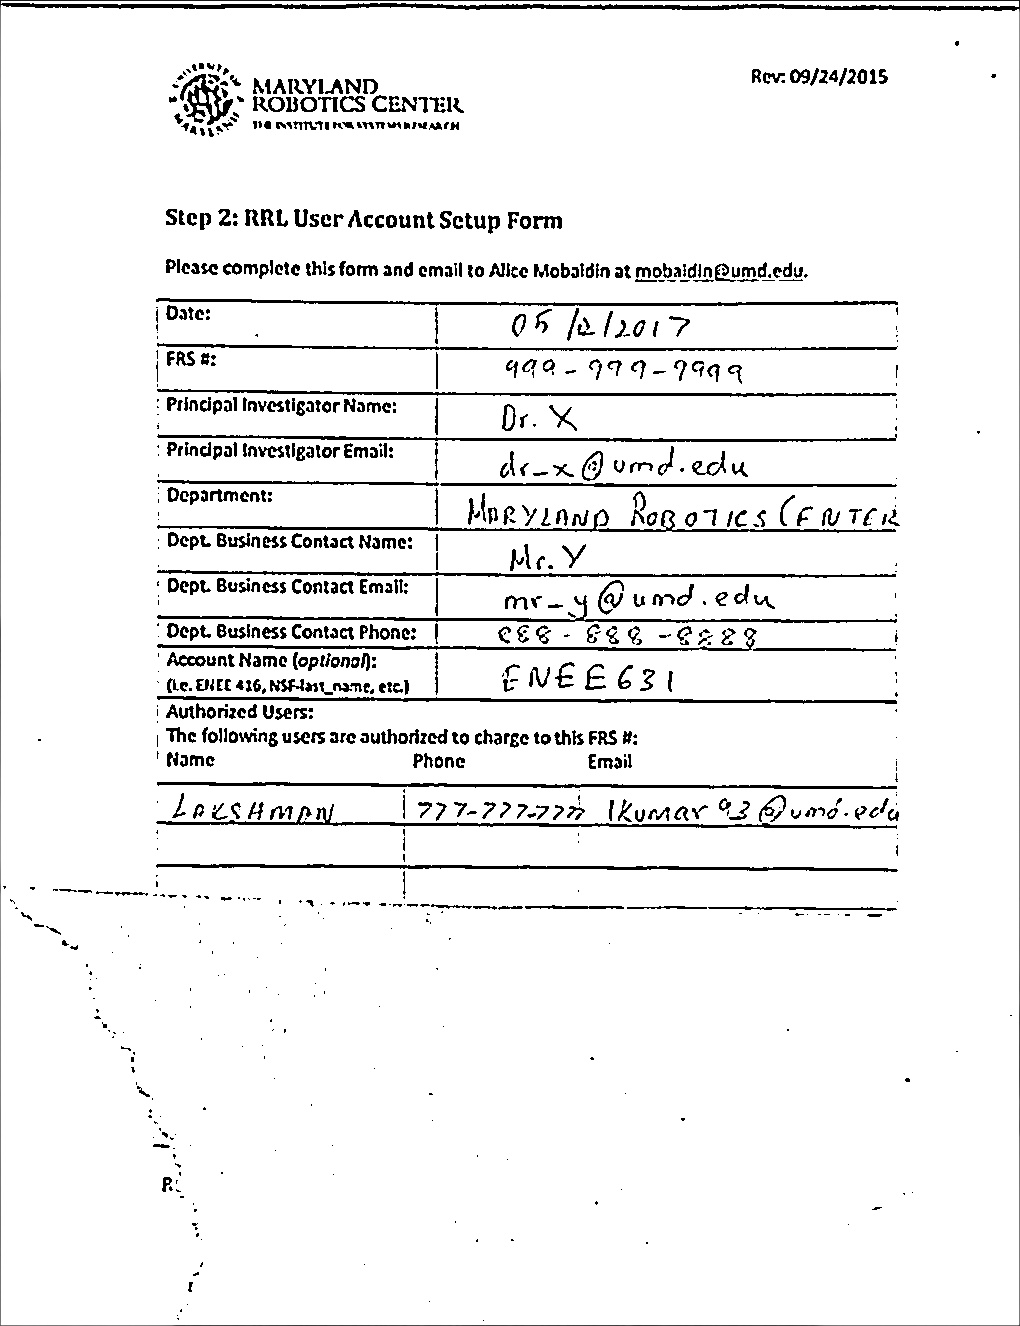
\includegraphics[height=18cm ]{Figures/thresholded_scanned_image}
	%	\decoRule
	\caption[Thresholded Scanned Document]{Thresholded Scanned Document.}
	\label{fig:ThresholdedScannedDocument}
\end{figure}

\pagebreak

Based on the values in both the thresholded images, the additional content in the scanned document is extracted from the reference document . The extracted foreground is then filtered a bit by dilation and median filtering. It can be seen from the image below that almost the entire filled content has been extracted. However, there might be some additional residue due to minute differences in alignment either because of Bilinear Interpolation or lesser number of iterations in RANSAC. \\ \\

\begin{figure}[th]
	\centering
	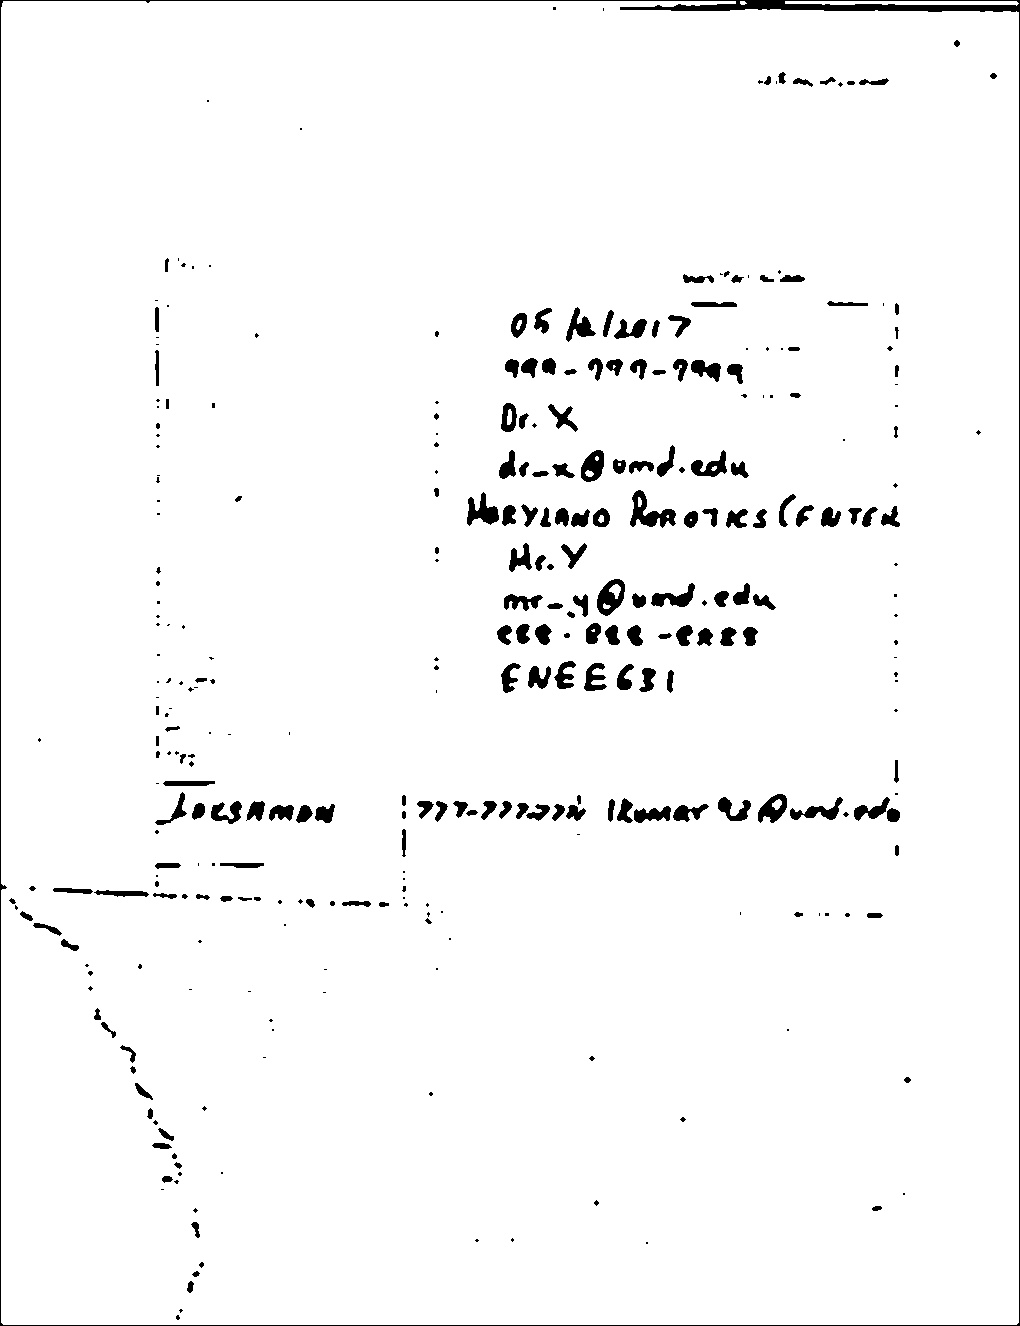
\includegraphics[height=18cm ]{Figures/background_subtraction}
	%	\decoRule
	\caption[Background Subtraction]{Background Subtraction.}
	\label{fig:BackgroundSubtraction}
\end{figure}
\pagebreak
\subsection{Foreground Addition}

Based on the extracted foreground, pixels in the scanned image are overlaid on top of the reference document. From the resultant images, it can be observed that most of the content is properly overlaid, however, there are some noises and artifacts due to border effects, minute differences in alignment, adaptive thresholding parameters and edges of obstructions in the image of scanned document. 
\\
\\
The binary version of the restored image is shown below. \\ 

\begin{figure}[th]
	\centering
	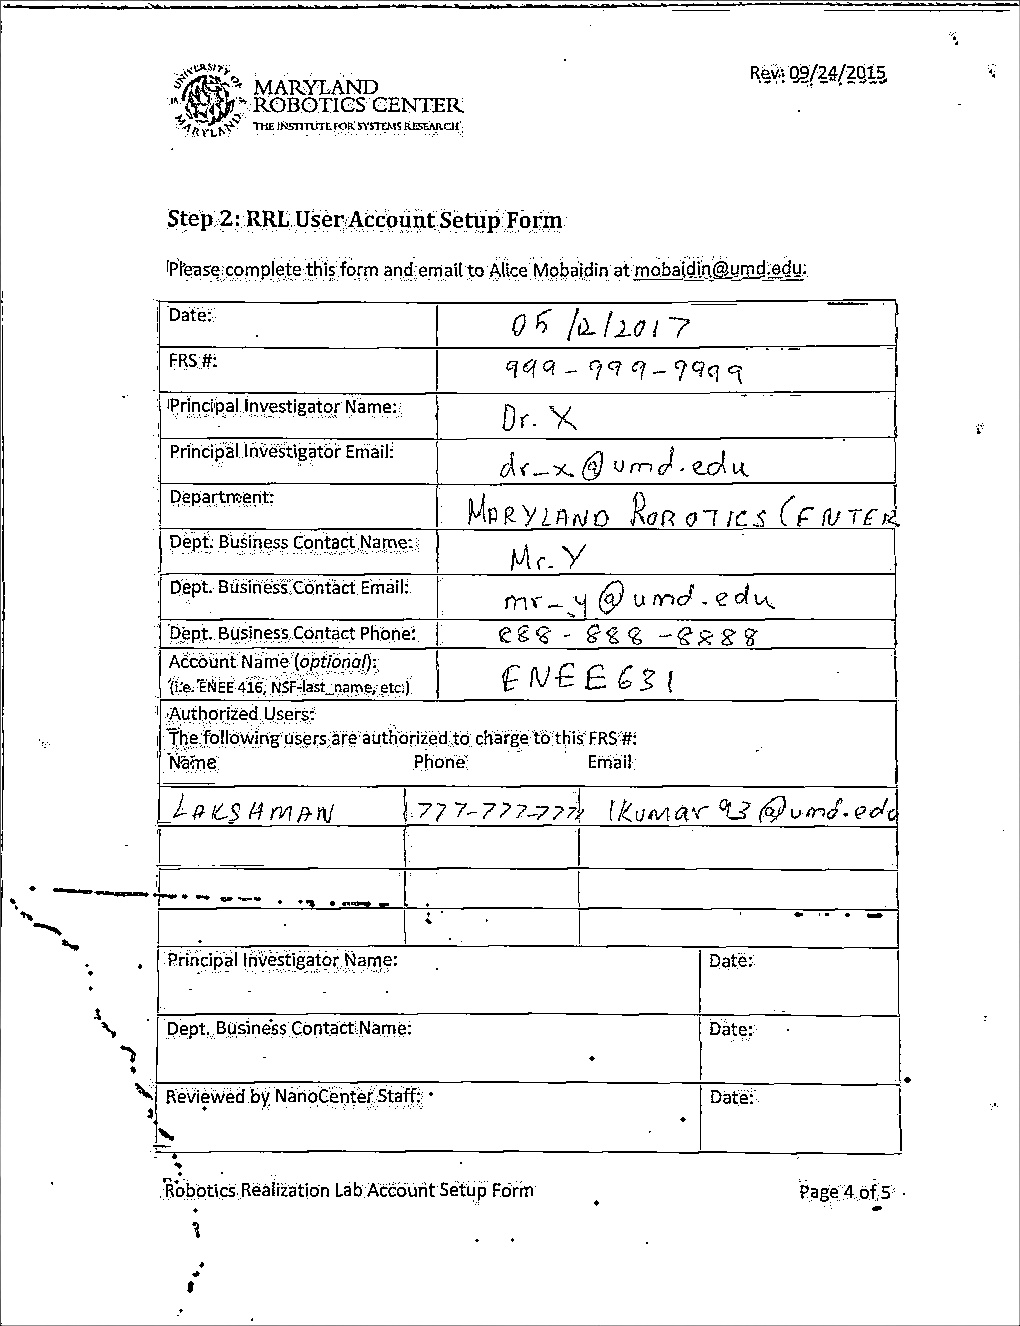
\includegraphics[height=16cm ]{Figures/thresholded_restored_image}
	%	\decoRule
	\caption[Binary Restored Image]{Binary Restored Image.}
	\label{fig:BinaryRestoredImage}
\end{figure}

\pagebreak

The RGB version of the restored image is shown below. \\  \\

\begin{figure}[th]
	\centering
	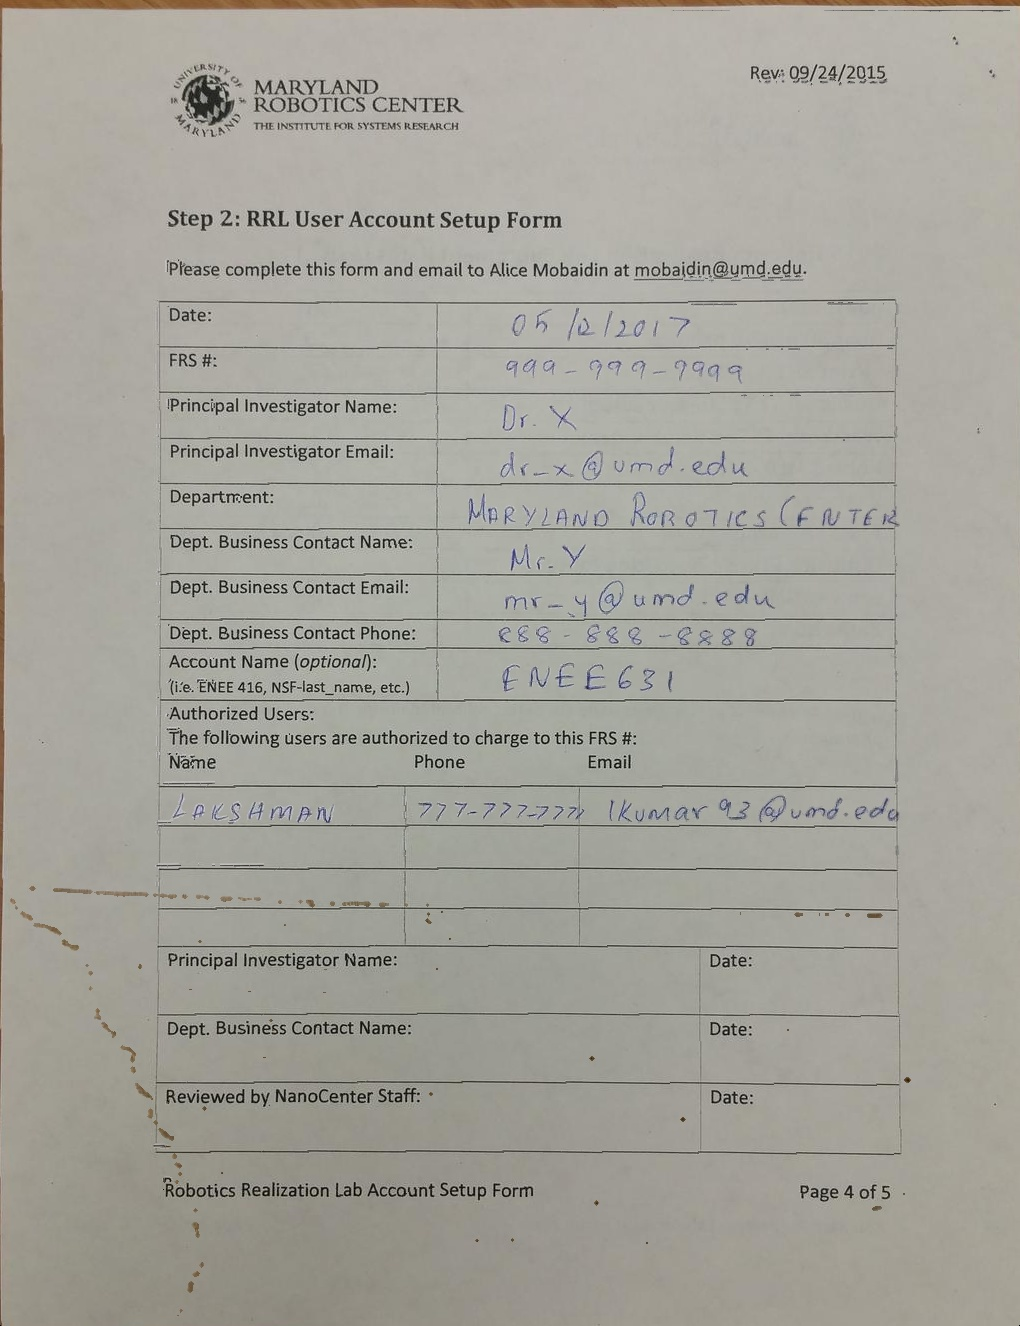
\includegraphics[height=18cm ]{Figures/restored_image}
	%	\decoRule
	\caption[Restored Image]{Restored Image.}
	\label{fig:RestoredImage}
\end{figure}

\pagebreak


%----------------------------------------------------------------------------------------



% Chapter 1

\chapter{Conclusion} % Main chapter title

\label{Chapter4} % For referencing the chapter elsewhere, use \ref{Chapter1} 

%------------------------------------------------------------------------

% Define some commands to keep the formatting separated from the content %------------------------------------------------------------------------

\section{Observations}
In this project, a sequential method to extract a document from an image and register it in order to do content extraction of the filled version of the same document has been laid out and implemented. Based on the experiments conducted as a part of this project, a few keen observations can be made as follows.
\begin{itemize}
	\item The technique works well as long as the \nameref{Assumptions} are satisfied.
	\item \nameref{Chapter2} takes roughly 5 to 7 seconds and \nameref{Chapter3} with Content Extraction takes roughly 15 to 25 seconds depending on the size and nature of the image. Hence totally the program takes about 30 seconds to execute.
	\item Sometimes specific tuning for parameters like Adaptive Thresholding Constant, Kernel Sizes, to suit a particular image is required.
	\item As \nameref{Assumptions} made do not require any sort of markings or specific ink color for the filled content, the output is not perfect .
	\item Background subtraction works well in-spite of having obstructions in the scanned image.
\end{itemize}
%----------------------------------------------------------------------------------------

\section{Future Works}

\begin{itemize}
	\item Optimize the code and algorithm to take less then 2 seconds to give the final output.
	\item Reduce the number of  \nameref{Assumptions} .
	\item Do additional filtering to remove artifacts due to border effects, obstructions and minute \\differences in image alignment.
	\item Automated tuning of certain parameters based on the nature of the image.
	\item Integrate OCR.
\end{itemize}


 
%\include{Chapters/Chapter5} 

%----------------------------------------------------------------------------------------
%	THESIS CONTENT - APPENDICES
%----------------------------------------------------------------------------------------

\appendix % Cue to tell LaTeX that the following "chapters" are Appendices

% Include the appendices of the thesis as separate files from the Appendices folder
% Uncomment the lines as you write the Appendices

% Appendix A

\chapter{Experimental Results} % Main appendix title

\label{AppendixA} % For referencing this appendix elsewhere, use \ref{AppendixA}

\section{Document Extraction}

Given below are few scanned images and their corresponding document extractions.

\begin{figure}[th]
	\centering
	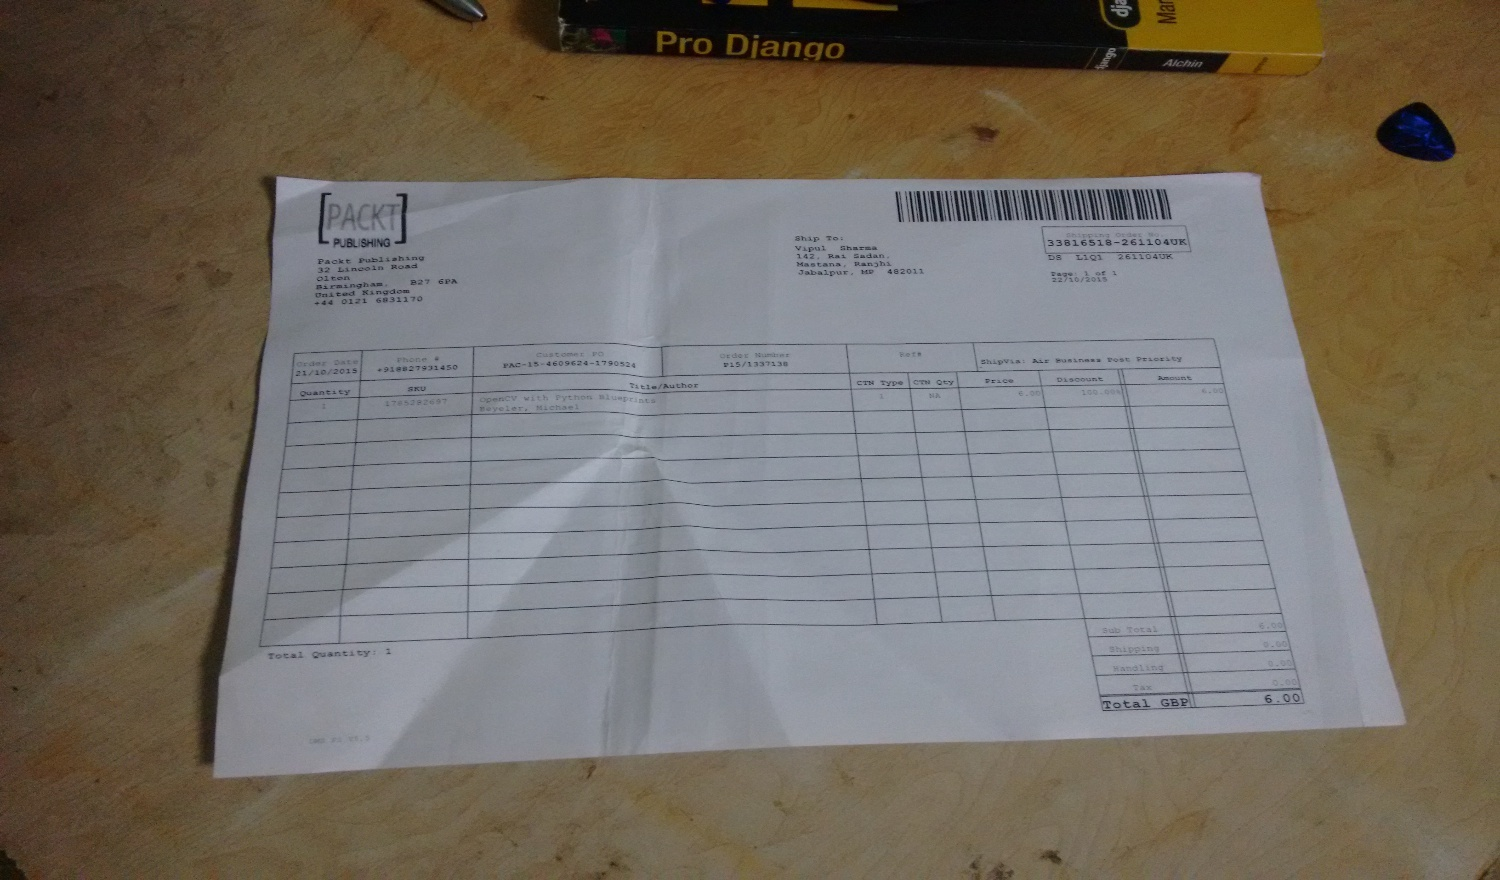
\includegraphics[height=8.8cm ]{Figures/scanned_image2}
	%	\decoRule
	\caption[Scanned Image 2]{Scanned Image 2 (Source : images.google.com).}
	\label{fig:ScannedImage2}
\end{figure}

\begin{figure}[th]
	\centering
	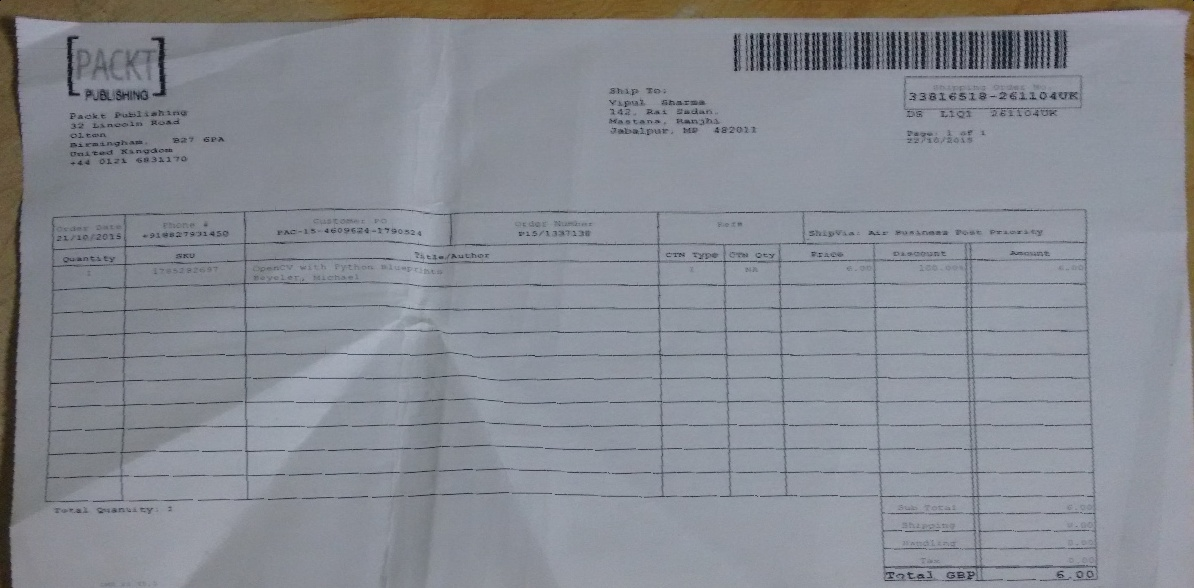
\includegraphics[height=7.5cm ]{Figures/warped_image2}
	%	\decoRule
	\caption[Warped Image 2]{Warped Image 2.}
	\label{fig:WarpedImage2}
\end{figure}

\pagebreak

\begin{figure}[th]
	\centering
	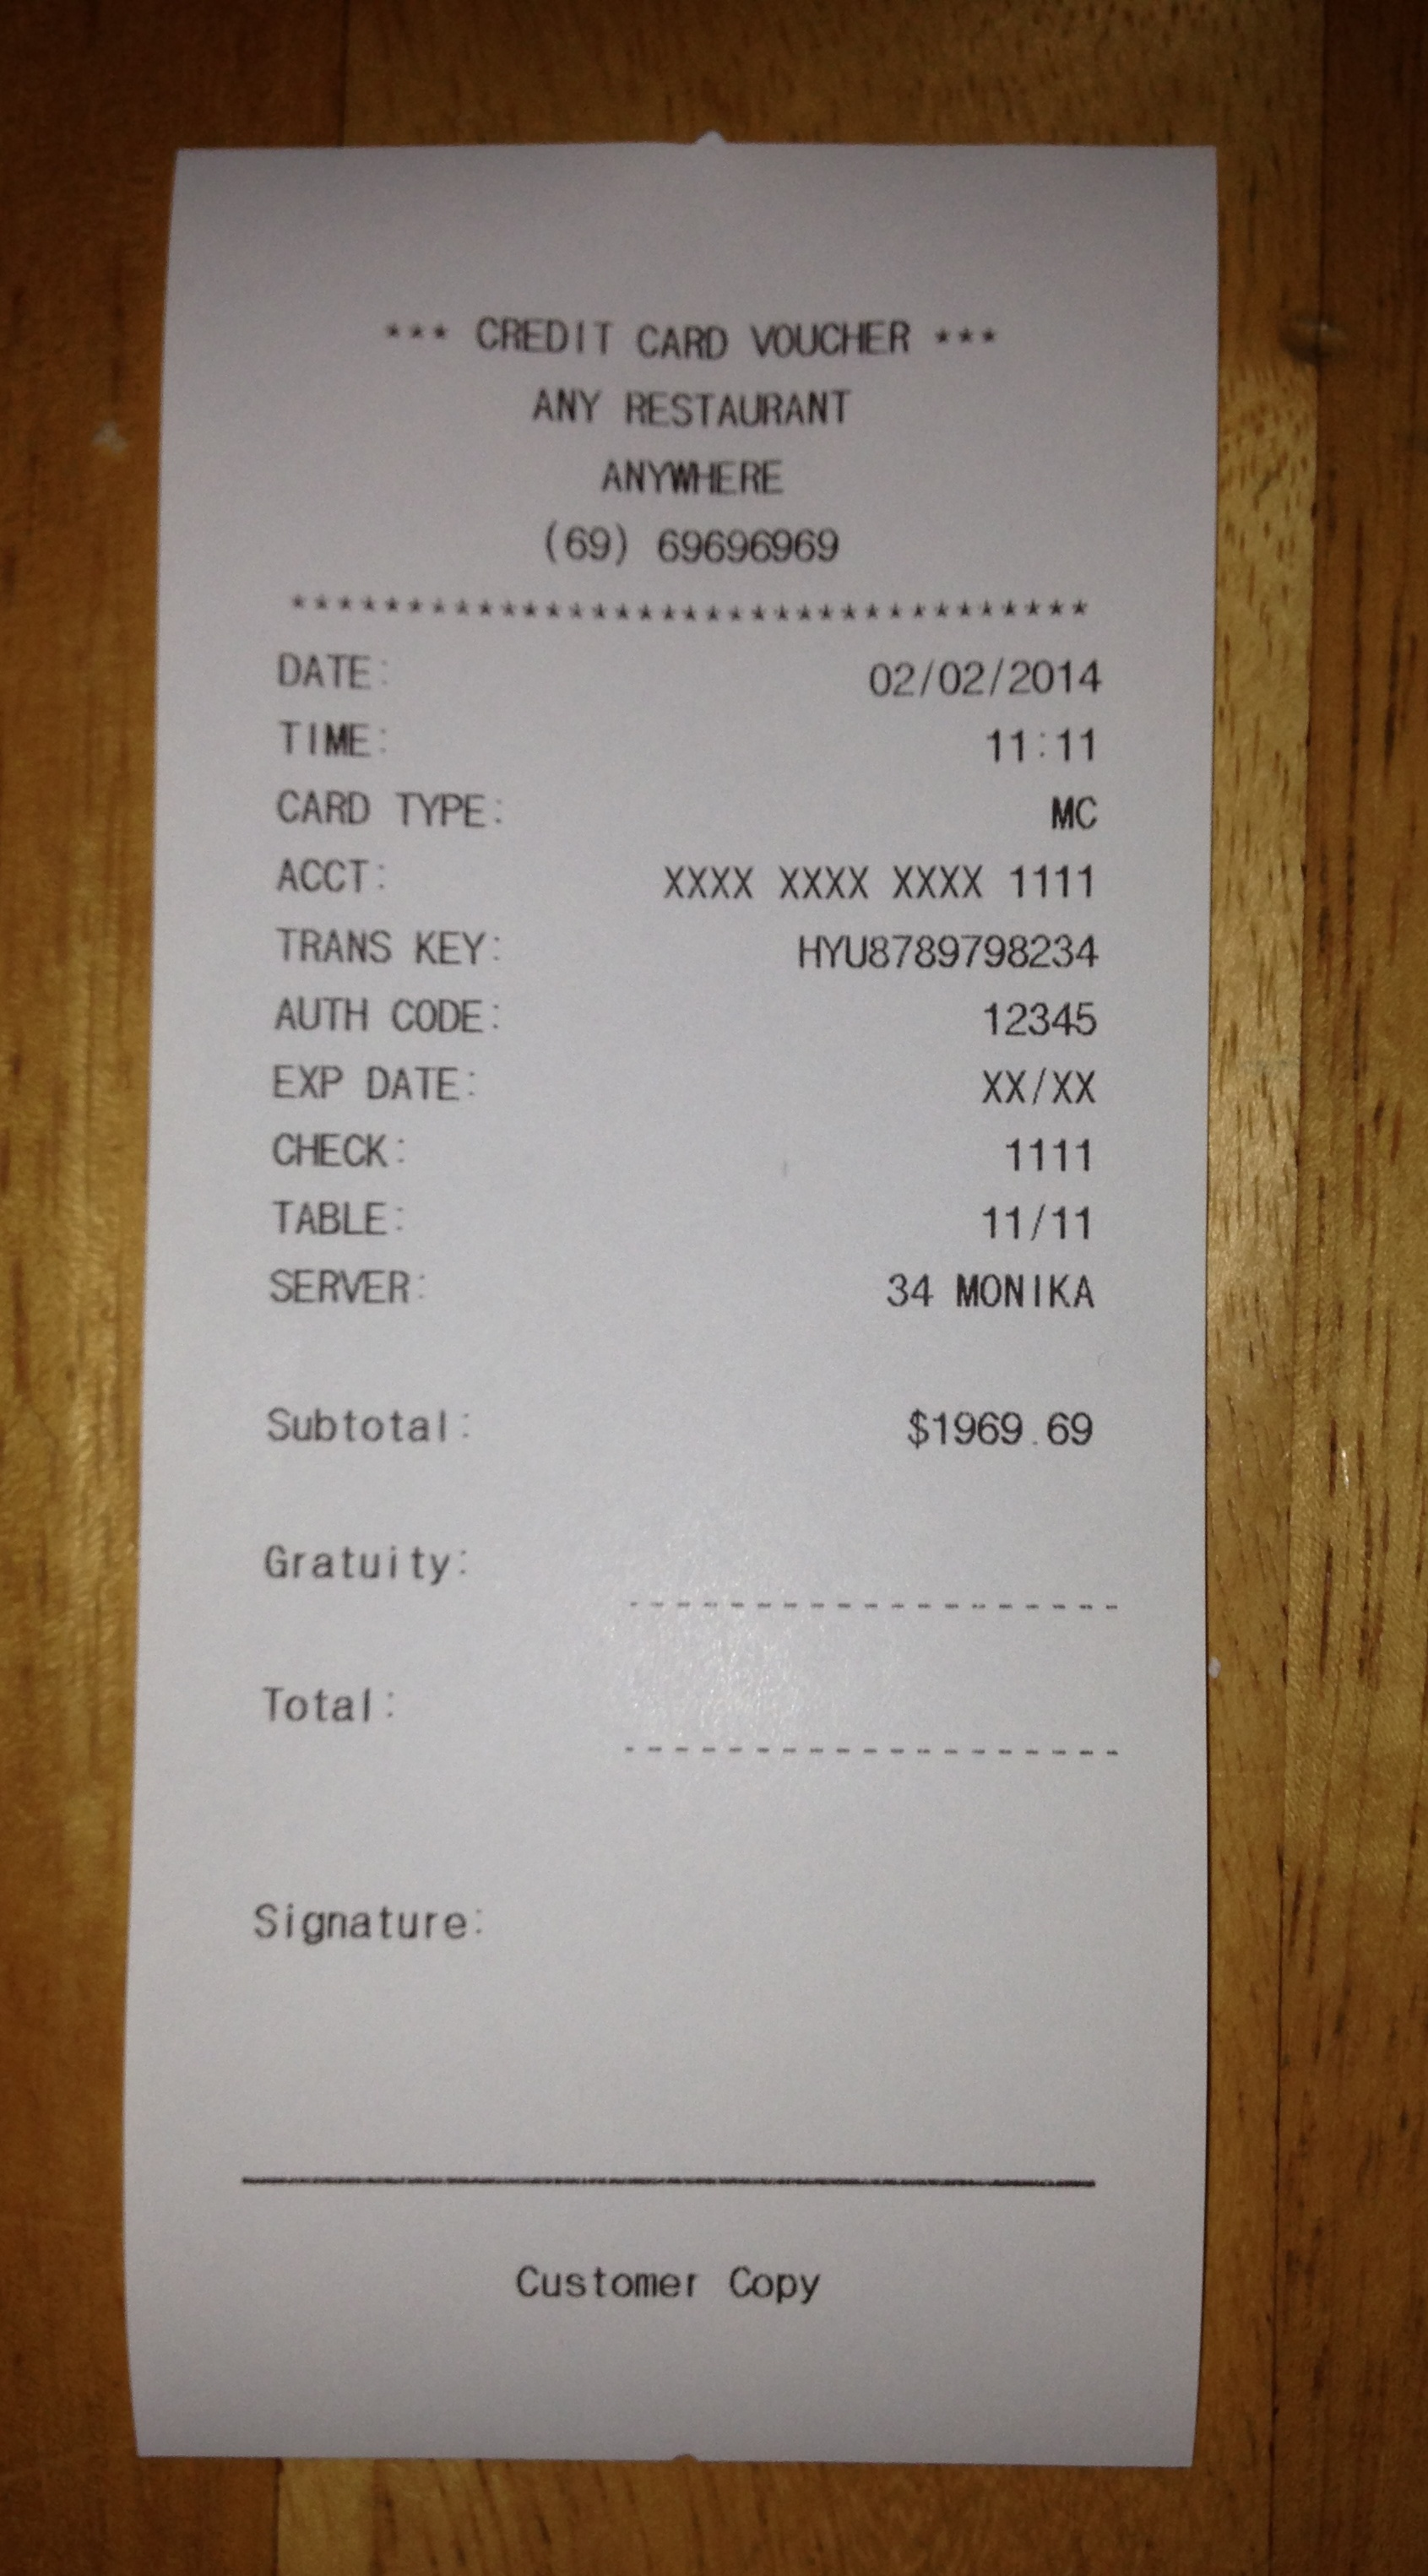
\includegraphics[height=8.5cm ]{Figures/scanned_image3}
	%	\decoRule
	\caption[Scanned Image 3]{Scanned Image 3 (Source : images.google.com).}
	\label{fig:ScannedImage3}
\end{figure}

\begin{figure}[th]
	\centering
	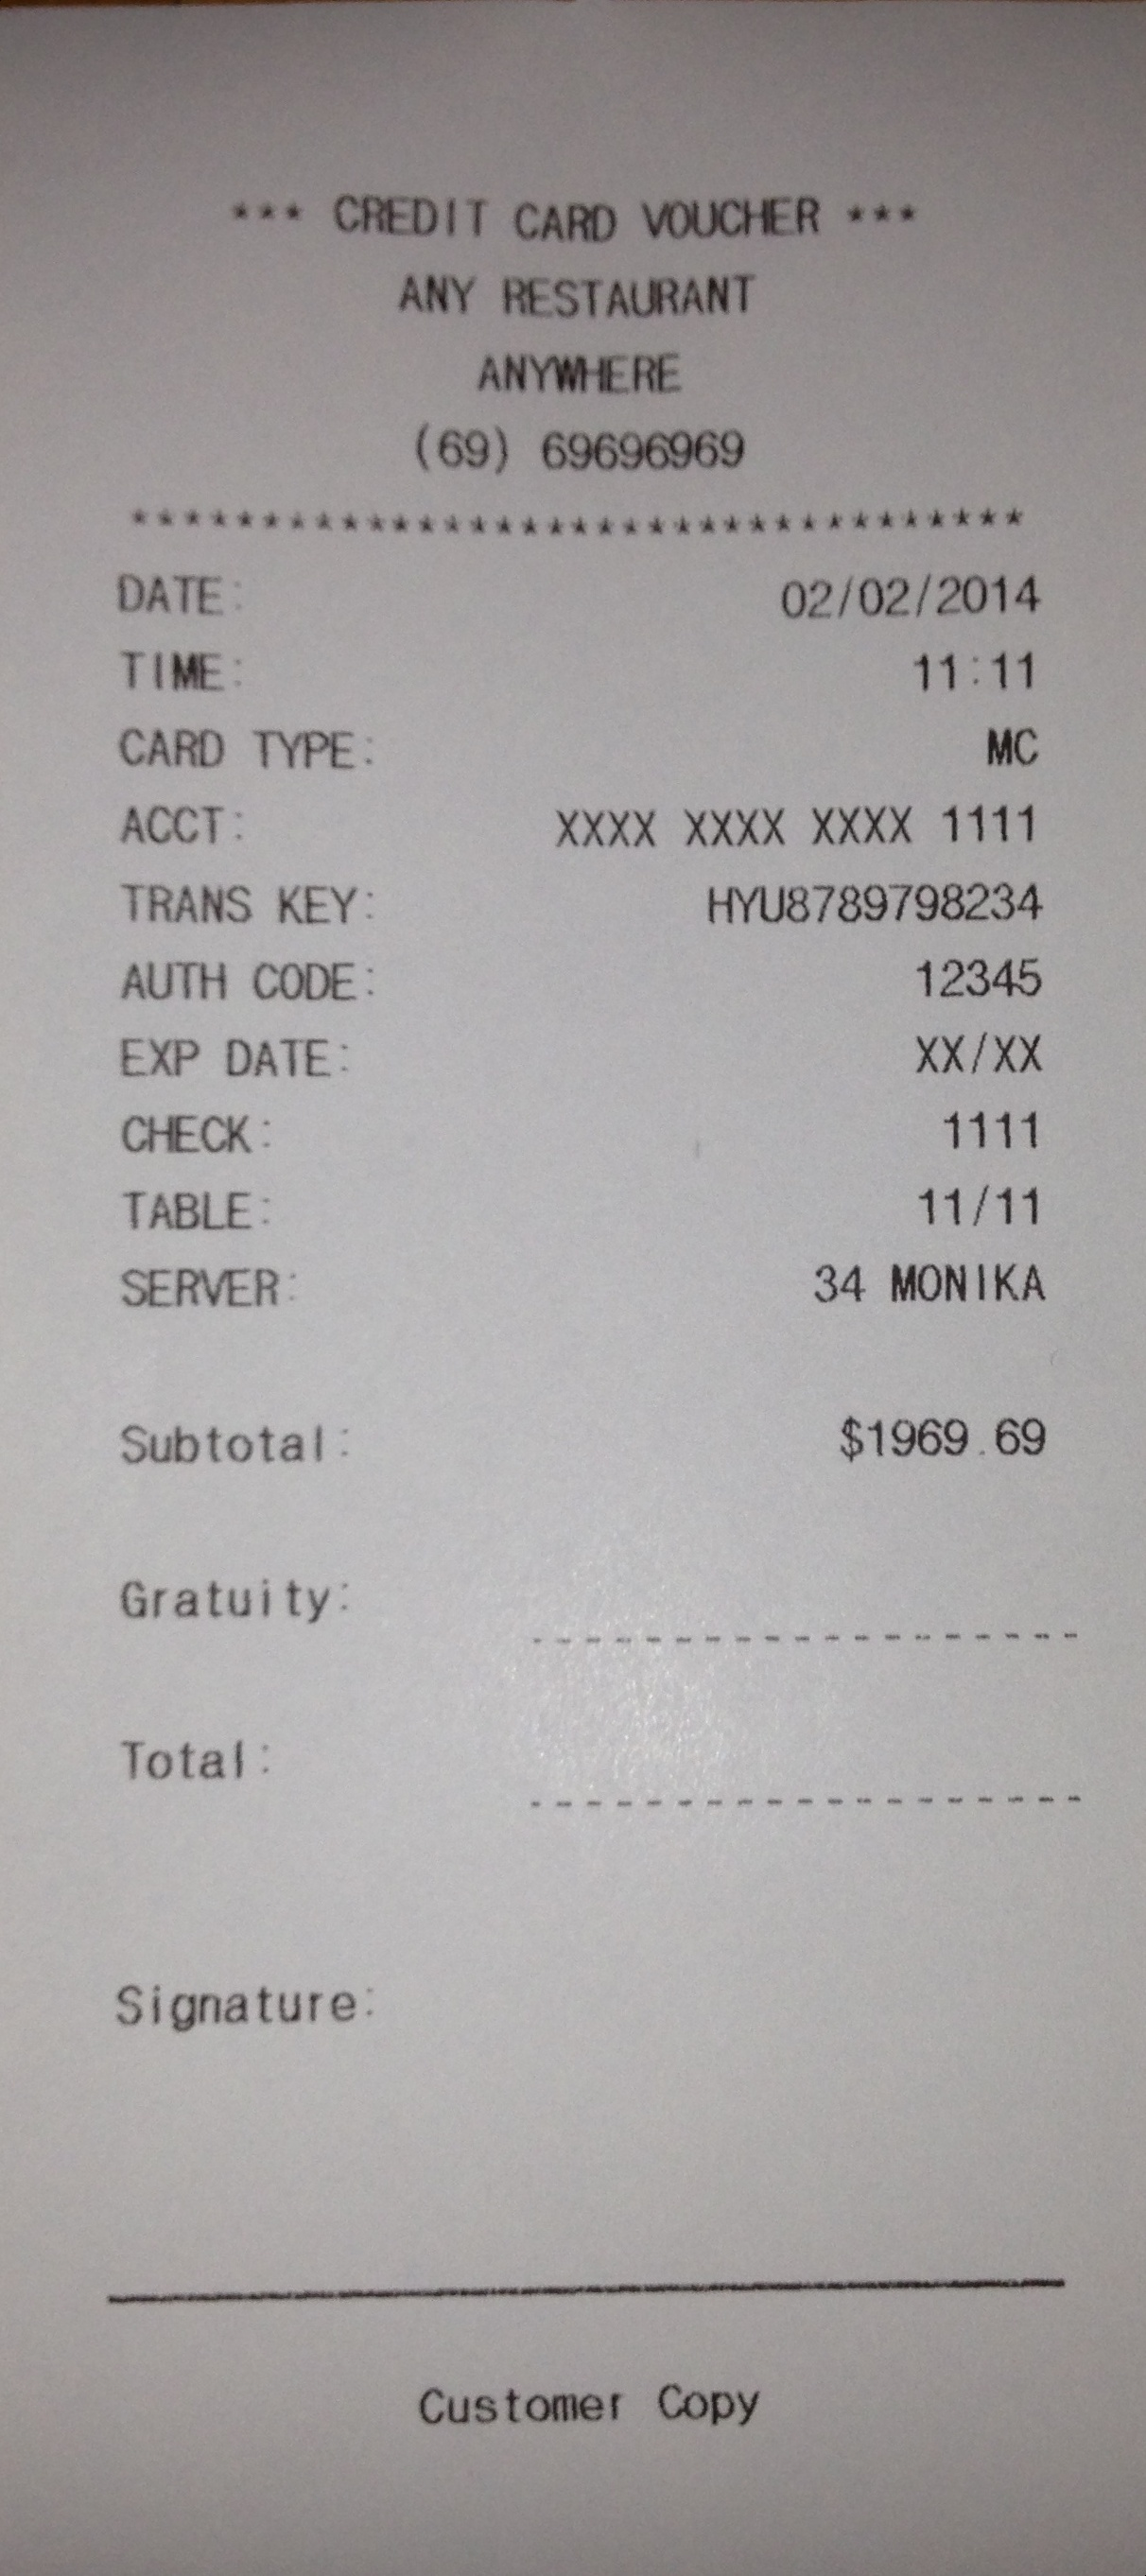
\includegraphics[height=8cm ]{Figures/warped_image3}
	%	\decoRule
	\caption[Warped Image 3]{Warped Image 3.}
	\label{fig:WarpedImage3}
\end{figure}

\pagebreak

\section{Image Registration}

Given below are few reference documents and scanned images and their corresponding image registrations/content extractions.

\begin{figure}[th]
	\centering
	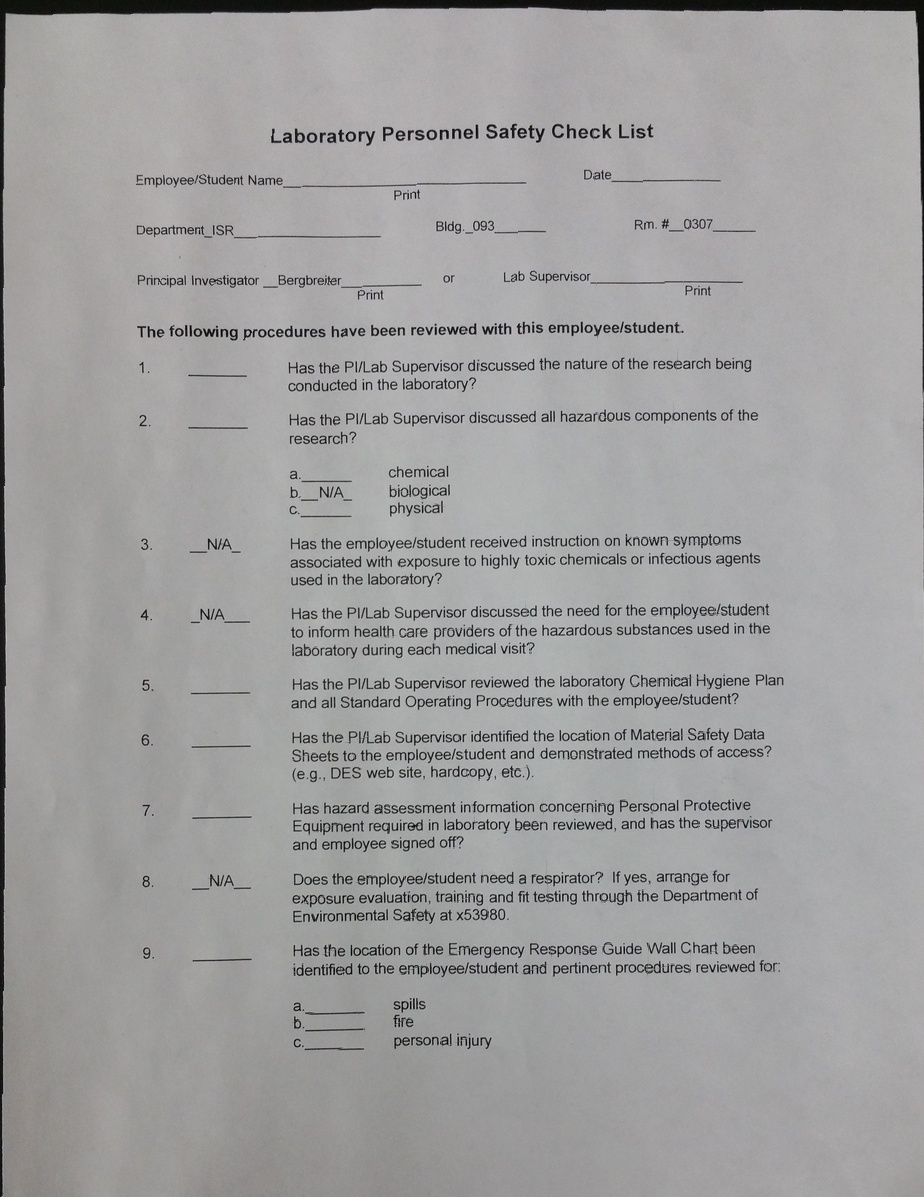
\includegraphics[height=18cm ]{Figures/reference_image2}
	%	\decoRule
	\caption[Reference Image 2]{Reference Image 2.}
	\label{fig:ReferenceImage2}
\end{figure}
\pagebreak
\begin{figure}[th]
	\centering
	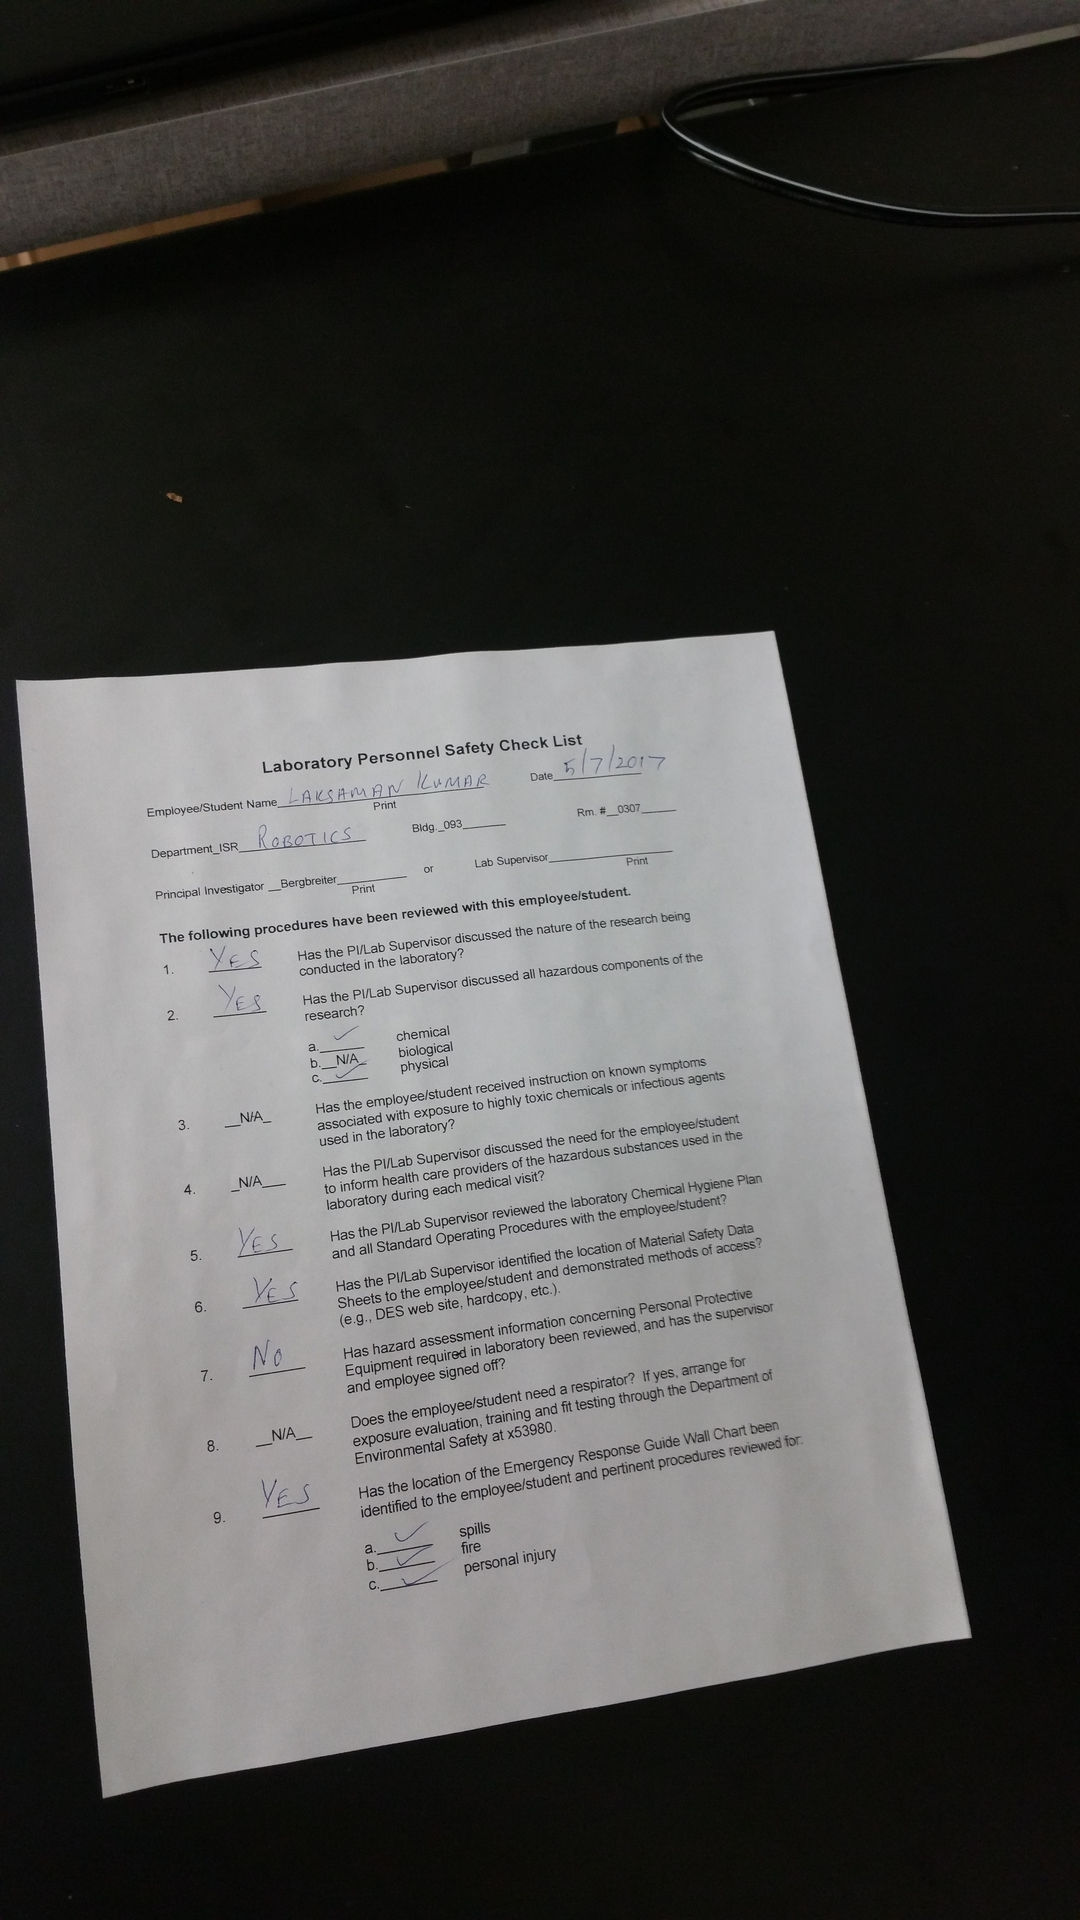
\includegraphics[height=19cm ]{Figures/filled_document1}
	%	\decoRule
	\caption[Filled Document]{Filled Document.}
	\label{fig:FilledDocument}
\end{figure}
\pagebreak
\begin{figure}[th]
	\centering
	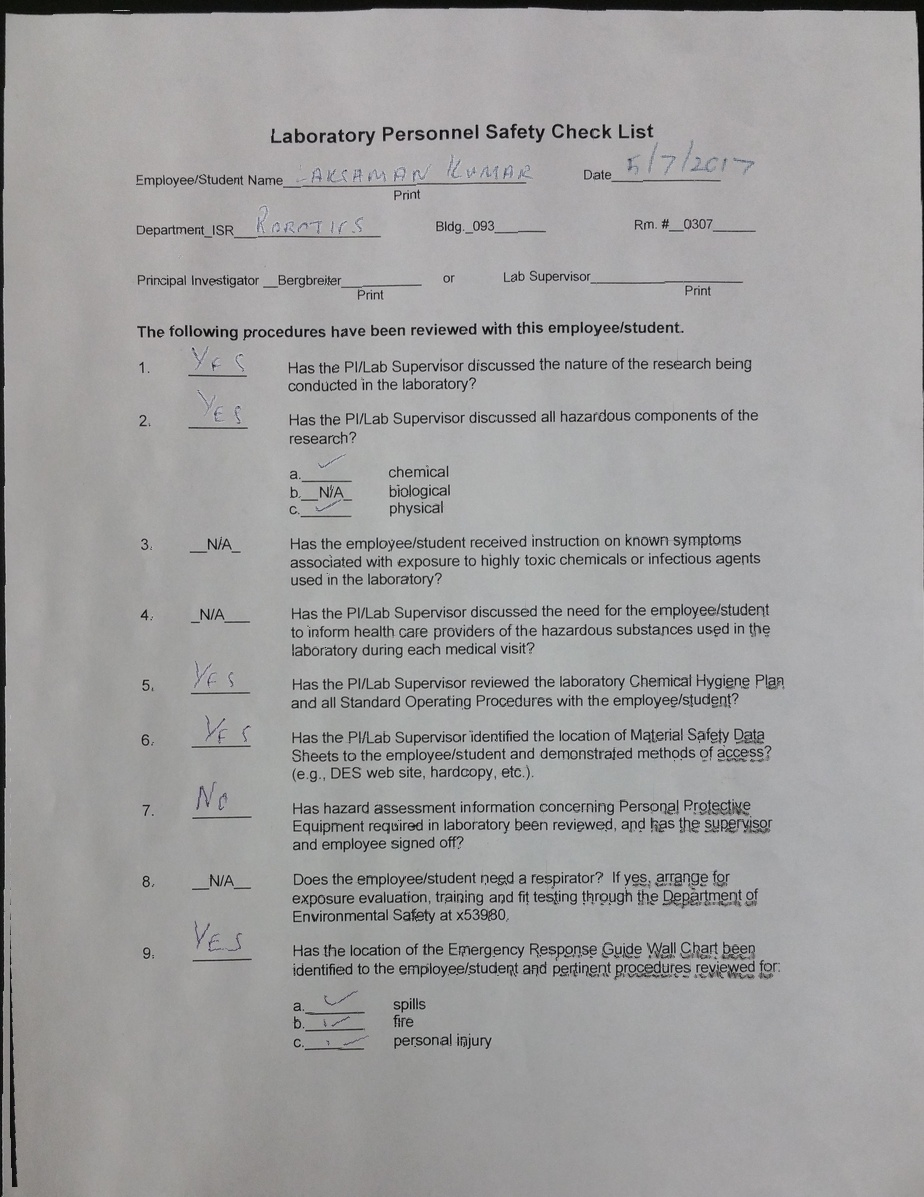
\includegraphics[height=19cm ]{Figures/restored_image2}
	%	\decoRule
	\caption[Restored Image 2]{Restored Image 2.}
	\label{fig:RestoredImage2}
\end{figure}
\pagebreak
\begin{figure}[th]
	\centering
	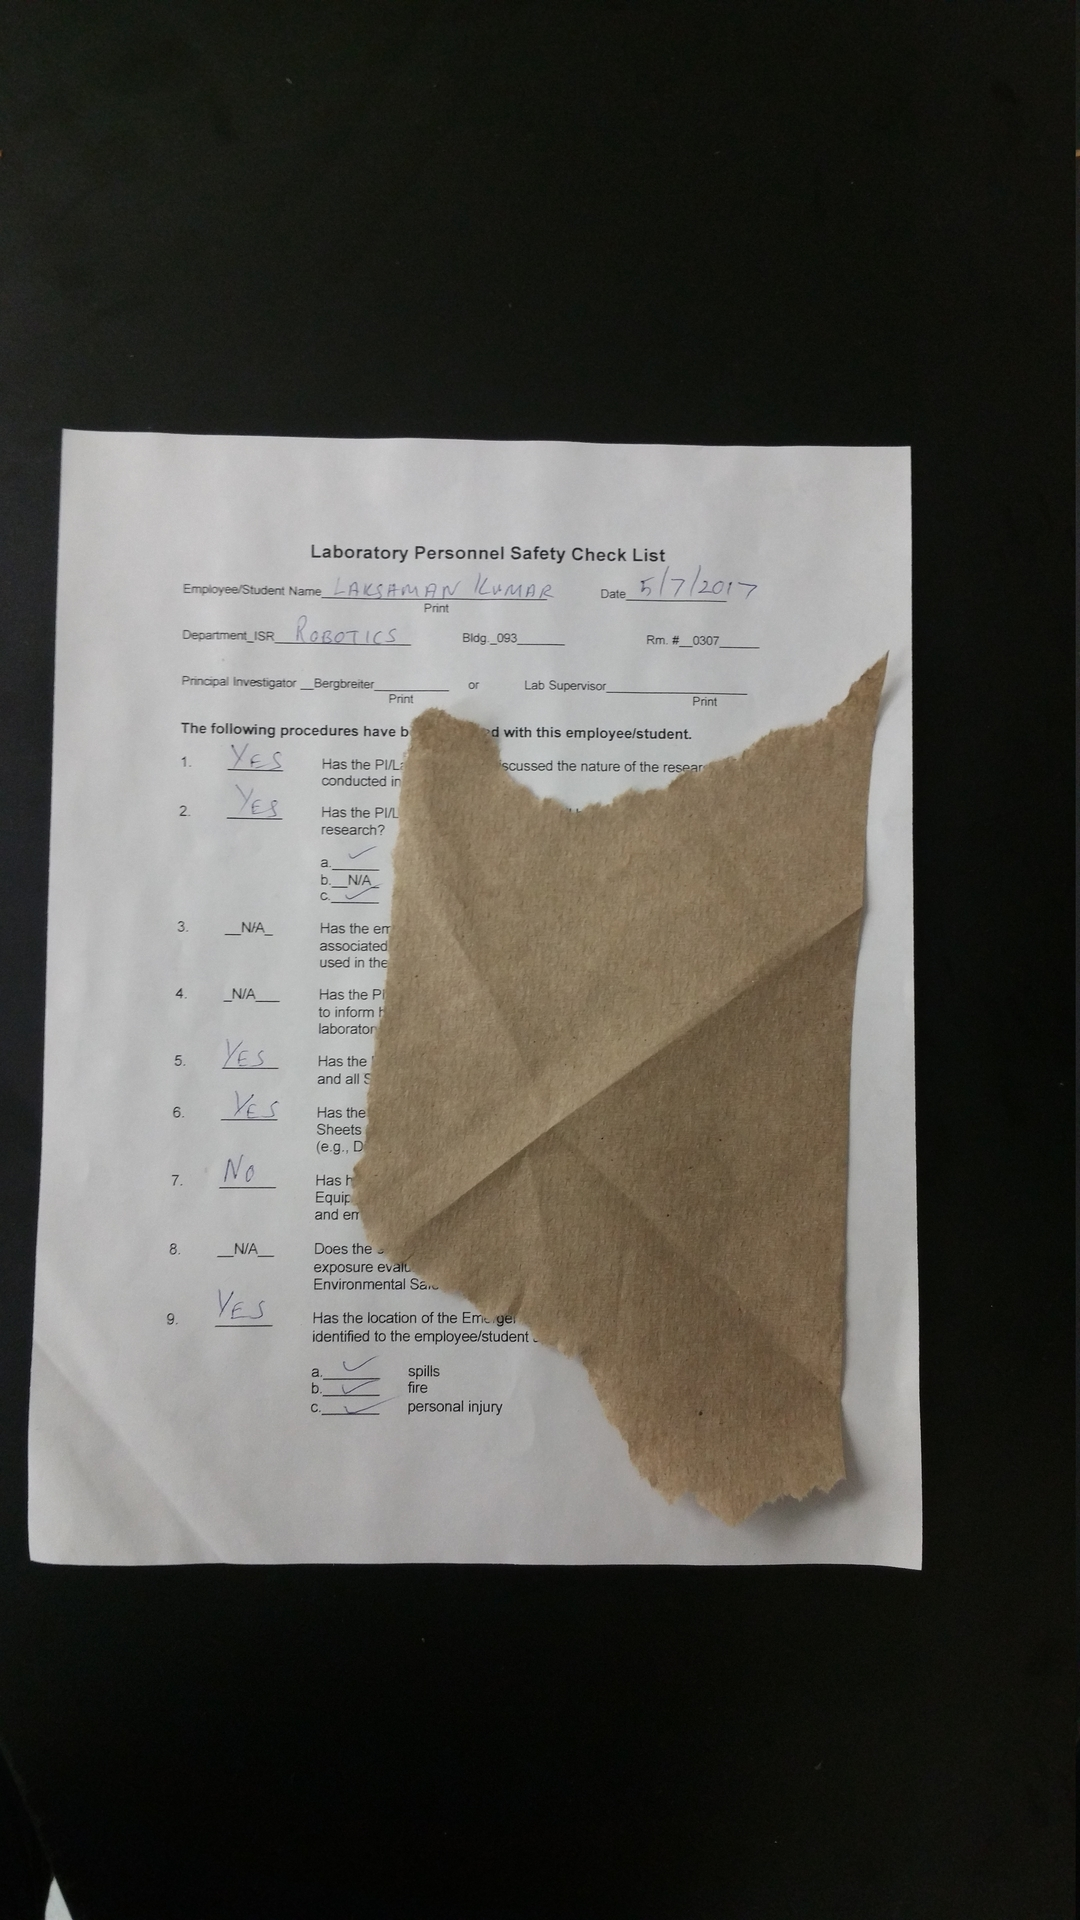
\includegraphics[height=19cm ]{Figures/filled_document2}
	%	\decoRule
	\caption[Filled Document 2]{Filled Document 2.}
	\label{fig:FilledDocument2}
\end{figure}
\pagebreak
\begin{figure}[th]
	\centering
	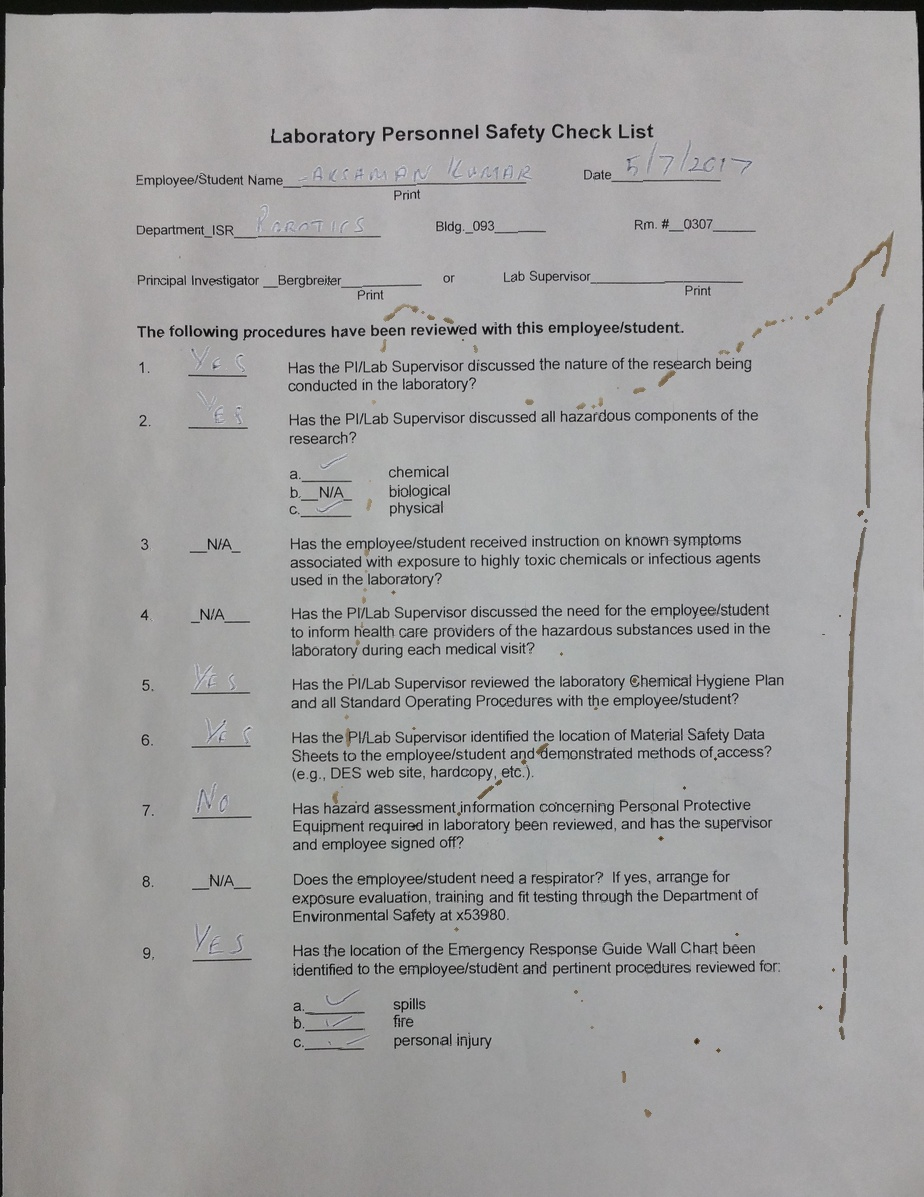
\includegraphics[height=19cm ]{Figures/restored_image3}
	%	\decoRule
	\caption[Restored Image 3]{Restored Image 3.}
	\label{fig:RestoredImage3}
\end{figure}

% Appendix A

\chapter{Source Code} % Main appendix title
\label{AppendixB}
The source code for the entire project can be found at \\
\url{https://github.com/lkumar93/Image-Processing/blob/master/mobile_scanner}
 % For referencing this appendix elsewhere, use \ref{AppendixB}

\section{Image Tranformation}

\subsection{Header}
\begin{lstlisting}
// image_transformation.h

#ifndef IMAGE_TRANSFORMATION_H_
#define IMAGE_TRANSFORMATION_H_

#include <iostream>
#include <opencv2/opencv.hpp>

using namespace cv;
using namespace std;

void bilinearInterpolation(Mat image, int vacant_pixel_value=0);
Mat perspective_transform(Point2f corner_points[], Point2f reference_points[]);
void warp_image(const Mat& input_image, Mat& output_image, const Mat& perspective_transform);
Mat resize_image(const Mat& input_image, int width, int height);

#endif // IMAGE_TRANSFORMATION_H


\end{lstlisting}

\subsection{Source}
\begin{lstlisting}
// image_transformation.cpp

#include "image_transformation.h"

void bilinearInterpolation(Mat image, int vacant_pixel_value)
{
if(image.type() == CV_8UC3)
{
Vec3b vacant_pixel;
vacant_pixel[0] = vacant_pixel_value;
vacant_pixel[1] = vacant_pixel_value;
vacant_pixel[2] = vacant_pixel_value;

for(int j = 0; j < image.rows ; j++)
{
for(int i = 0; i < image.cols; i++)
{
if(image.at<Vec3b>(j, i) == vacant_pixel)
{
int count_r = i;
//get right most filled_neighbour
while( image.at<Vec3b>(j, count_r) == vacant_pixel && count_r< image.cols)
{
count_r++;
}
int count_l = i;
//get left most filled_neighbour
while( image.at<Vec3b>(j, count_l) == vacant_pixel && count_l >= 0 )
{
count_l--;
}

int count_b = j;
//get bottom most filled_neighbour
while( image.at<Vec3b>(count_b, i) == vacant_pixel && count_b < image.rows )
{
count_b++;
}

int count_t = j;
//get top most filled_neighbour
while( image.at<Vec3b>(count_t, i) == vacant_pixel && count_t >= 0 )
{
count_t--;
}

if(count_r >=image.cols)
count_r = image.cols-1;

if(count_l < 0)
count_l = 0;

if(count_b >=image.rows)
count_b = image.rows-1;

if(count_t < 0)
count_t = 0;


float left_offset = i-count_l;
float right_offset = count_r-i;

float top_offset = j-count_t;
float bottom_offset = count_b-j;

float col_offset = left_offset+right_offset;
float row_offset = top_offset+bottom_offset;

if(col_offset > 0)
{
left_offset = (1-left_offset/col_offset)/2.0;
right_offset = (1-right_offset/col_offset)/2.0;
}

if(row_offset >0)
{
top_offset = (1-top_offset/row_offset)/2.0;
bottom_offset = (1-bottom_offset/row_offset)/2.0;
}

Vec3b top_pixel = image.at<Vec3b>(count_t, i);
Vec3b bottom_pixel = image.at<Vec3b>(count_b, i);

Vec3b right_pixel = image.at<Vec3b>(j, count_r);
Vec3b left_pixel = image.at<Vec3b>(j, count_l);

Vec3b interpolated_value;

if(left_pixel == vacant_pixel)
left_offset = 0;

if(right_pixel == vacant_pixel)
right_offset = 0;

if(top_pixel == vacant_pixel)
top_offset = 0;

if(bottom_pixel == vacant_pixel)
bottom_offset = 0;

col_offset = left_offset+right_offset;
row_offset = top_offset+bottom_offset;

if(col_offset > 0)
{
left_offset = left_offset/(2*col_offset);
right_offset = right_offset/(2*col_offset);
}


if(row_offset >0)
{
top_offset = top_offset/(2*row_offset);
bottom_offset = bottom_offset/(2*row_offset);
}


float total = left_offset + right_offset + top_offset +bottom_offset;

if(total > 0)
{
left_offset/=total;
right_offset/=total;
top_offset/=total;
bottom_offset/=total;	
}			

interpolated_value[0] = left_offset*left_pixel[0] + right_offset*right_pixel[0] + top_offset*top_pixel[0]
+ bottom_offset*bottom_pixel[0];

interpolated_value[1] = left_offset*left_pixel[1] + right_offset*right_pixel[1] + top_offset*top_pixel[1]
+ bottom_offset*bottom_pixel[1];

interpolated_value[2] = left_offset*left_pixel[2] + right_offset*right_pixel[2] + top_offset*top_pixel[2]
+ bottom_offset*bottom_pixel[2];

image.at<Vec3b>(j, i) = interpolated_value;
}
}
}
}
else if(image.type() == CV_8UC1)
{

// Bilinear Interpolation
for(int j = 0; j < image.rows ; j++)
{
for(int i = 0; i < image.cols; i++)
{
if(image.at<uchar>(j, i) == vacant_pixel_value)
{
int count_r = i;
//get right most filled_neighbour
while( image.at<uchar>(j, count_r) == vacant_pixel_value && count_r< image.cols)
{
count_r++;
}
int count_l = i;
//get left most filled_neighbour
while( image.at<uchar>(j, count_l) == vacant_pixel_value && count_l >= 0 )
{
count_l--;
}

int count_b = j;
//get bottom most filled_neighbour
while( image.at<uchar>(count_b, i) == vacant_pixel_value && count_b < image.rows )
{
count_b++;
}

int count_t = j;
//get top most filled_neighbour
while( image.at<uchar>(count_t, i) == vacant_pixel_value && count_t >= 0 )
{
count_t--;
}

if(count_r >=image.cols)
count_r = image.cols-1;

if(count_l < 0)
count_l = 0;

if(count_b >=image.rows)
count_b = image.rows-1;

if(count_t < 0)
count_t = 0;


float left_offset = i-count_l;
float right_offset = count_r-i;

float top_offset = j-count_t;
float bottom_offset = count_b-j;

float col_offset = left_offset+right_offset;
float row_offset = top_offset+bottom_offset;

if(col_offset > 0)
{
left_offset = (1-left_offset/col_offset)/2.0;
right_offset = (1-right_offset/col_offset)/2.0;
}

if(row_offset >0)
{
top_offset = (1-top_offset/row_offset)/2.0;
bottom_offset = (1-bottom_offset/row_offset)/2.0;
}

int top_pixel = image.at<uchar>(count_t, i);
int bottom_pixel = image.at<uchar>(count_b, i);

int right_pixel = image.at<uchar>(j, count_r);
int left_pixel = image.at<uchar>(j, count_l);

int interpolated_value;

if(left_pixel == vacant_pixel_value)
left_offset = 0;

if(right_pixel == vacant_pixel_value)
right_offset = 0;

if(top_pixel == vacant_pixel_value)
top_offset = 0;

if(bottom_pixel == vacant_pixel_value)
bottom_offset = 0;

if(col_offset > 0)
{
left_offset = left_offset/(2*col_offset);
right_offset = right_offset/(2*col_offset);
}


if(row_offset >0)
{
top_offset = top_offset/(2*row_offset);
bottom_offset = bottom_offset/(2*row_offset);
}


float total = left_offset + right_offset + top_offset +bottom_offset;

if(total > 0)
{
left_offset/=total;
right_offset/=total;
top_offset/=total;
bottom_offset/=total;	
}			


interpolated_value = left_offset*left_pixel + right_offset*right_pixel + top_offset*top_pixel
+ bottom_offset*bottom_pixel;

image.at<uchar>(j, i) = interpolated_value;	
}
}
}
}
}

Mat perspective_transform(Point2f input_rectangle[], Point2f output_rectangle[])
{
Mat A = Mat::ones( 3, 3, CV_32F );
Mat B = Mat::ones( 3, 1, CV_32F );

A.at<float>(0,0) = input_rectangle[0].x;
A.at<float>(1,0) = input_rectangle[0].y;

A.at<float>(0,1) = input_rectangle[1].x;
A.at<float>(1,1) = input_rectangle[1].y;

A.at<float>(0,2) = input_rectangle[2].x;
A.at<float>(1,2) = input_rectangle[2].y;

B.at<float>(0,0) = input_rectangle[3].x;
B.at<float>(1,0) = input_rectangle[3].y;

Mat C = Mat::ones( 3, 1, CV_32F );
C = A.inv()*B;

Mat M = Mat::ones( 3, 3, CV_32F );

M.at<float>(0,0) = C.at<float>(0,0)*input_rectangle[0].x;
M.at<float>(1,0) =  C.at<float>(0,0)*input_rectangle[0].y;
M.at<float>(2,0) =  C.at<float>(0,0);

M.at<float>(0,1) =  C.at<float>(1,0)* input_rectangle[1].x;
M.at<float>(1,1) =  C.at<float>(1,0)*input_rectangle[1].y;
M.at<float>(2,1) =  C.at<float>(1,0);

M.at<float>(0,2) =  C.at<float>(2,0)*input_rectangle[2].x;
M.at<float>(1,2) =  C.at<float>(2,0)*input_rectangle[2].y;
M.at<float>(2,2) =  C.at<float>(2,0);

Mat D = Mat::ones( 3, 3, CV_32F );
Mat E = Mat::ones( 3, 1, CV_32F );

D.at<float>(0,0) = output_rectangle[0].x;
D.at<float>(1,0) = output_rectangle[0].y;

D.at<float>(0,1) = output_rectangle[1].x;
D.at<float>(1,1) = output_rectangle[1].y;

D.at<float>(0,2) = output_rectangle[2].x;
D.at<float>(1,2) = output_rectangle[2].y;

E.at<float>(0,0) = output_rectangle[3].x;
E.at<float>(1,0) = output_rectangle[3].y;

Mat F = Mat::ones( 3, 1, CV_32F );
F = D.inv()*E;

Mat N = Mat::ones( 3, 3	, CV_32F );

N.at<float>(0,0) = F.at<float>(0,0)*output_rectangle[0].x;
N.at<float>(1,0) = F.at<float>(0,0)*output_rectangle[0].y;
N.at<float>(2,0) = F.at<float>(0,0);

N.at<float>(0,1) = F.at<float>(1,0)*output_rectangle[1].x;
N.at<float>(1,1) = F.at<float>(1,0)*output_rectangle[1].y;
N.at<float>(2,1) = F.at<float>(1,0);

N.at<float>(0,2) = F.at<float>(2,0)*output_rectangle[2].x;
N.at<float>(1,2) = F.at<float>(2,0)*output_rectangle[2].y;
N.at<float>(2,2) = F.at<float>(2,0);


Mat perspective_transform= Mat::ones( 3, 3, CV_32F );
perspective_transform = N*M.inv();

return perspective_transform;
}

Mat resize_image(const Mat& input_image, int width, int height)
{
Mat resized_image ;

float scale_x = (float)height/(float)input_image.rows;
float scale_y = (float)width/(float)input_image.cols;

if(input_image.type() == CV_8UC3)
{
resized_image = Mat::ones(height,width,CV_8UC3)*0;

for( int j = 0; j <  input_image.rows ; j++ )
for( int i = 0; i <  input_image.cols; i++ )
{
int x = cvFloor(scale_x*j);
int y = cvFloor(scale_y*i);

if(x >= 0 && x < height && y >=0 && y< width)
resized_image.at<Vec3b>(x,y) = input_image.at<Vec3b>(j,i);

}
}
else if(input_image.type() == CV_8UC1)
{
resized_image = Mat::ones(height,width,CV_8UC1)*0;

for( int j = 0; j <  input_image.rows ; j++ )
for( int i = 0; i <  input_image.cols; i++ )
{
int x = cvFloor(scale_x*j);
int y = cvFloor(scale_y*i);

if(x >= 0 && x < height && y >=0 && y< width)
resized_image.at<uchar>(x,y) = input_image.at<uchar>(j,i);

}
}

else
{
cout<<"Resize operation not available for this image type"<<endl;
return resized_image;
}

bilinearInterpolation(resized_image,0);

return resized_image;

}

void warp_image(const Mat& input_image, Mat& output_image, const Mat& perspective_transform)
{

Mat given_point = Mat::ones(3,1,CV_32F); 
Mat transformed_point = Mat::ones(3,1,CV_32F);

if(input_image.type() == CV_8UC3)
{
for( int j = 0; j <  input_image.rows ; j++ )
for( int i = 0; i <  input_image.cols; i++ )
{
given_point.at<float>(0,0) = i;
given_point.at<float>(1,0) = j;

transformed_point = perspective_transform*given_point;

int x = cvFloor(transformed_point.at<float>(1,0)/transformed_point.at<float>(2,0));
int y = cvFloor(transformed_point.at<float>(0,0)/transformed_point.at<float>(2,0));

if(x >= 0 && x < output_image.rows && y >=0 && y< output_image.cols)
output_image.at<Vec3b>(x,y) = input_image.at<Vec3b>(j,i);

}

}
else if(input_image.type() == CV_8UC1)
{
for( int j = 0; j <  input_image.rows ; j++ )
for( int i = 0; i <  input_image.cols; i++ )
{
given_point.at<float>(0,0) = i;
given_point.at<float>(1,0) = j;

transformed_point = perspective_transform*given_point;

int x = cvFloor(transformed_point.at<float>(1,0)/transformed_point.at<float>(2,0));
int y = cvFloor(transformed_point.at<float>(0,0)/transformed_point.at<float>(2,0));

if(x >= 0 && x < output_image.rows && y >=0 && y< output_image.cols)
output_image.at<uchar>(x,y) = input_image.at<uchar>(j,i);

}
}

}



\end{lstlisting}

\pagebreak
\section{Image Enhancement}

\subsection{Header}
\begin{lstlisting}
// image_enhancement.h

#ifndef IMAGE_ENHANCEMENT_H_
#define IMAGE_ENHANCEMENT_H_

#include <iostream>
#include <opencv2/opencv.hpp>

#define R_WEIGHT 0.2989
#define G_WEIGHT 0.5870
#define B_WEIGHT 0.1140

using namespace cv;

Mat convert_to_grayscale(const Mat& input_image);
void compute_histogram(const Mat& input_image, int histogram[]);
void display_histogram(int histogram[], const char* name);
void compute_cumulative_histogram(int histogram[], int cumulative_histogram[]);
int scale_histogram(int cumulative_histogram[],int scaled_histogram[], float scaling_factor);
Mat equalize_image(const Mat& input_image);
Mat log_transformation(const Mat& input_image, int transformation_constant);
Mat inverse_transformation(const Mat& input_image);
Mat gamma_correction(const Mat& input_image, int gamma);
Mat sharpen(const Mat& input_image, int kernel_size, float alpha);
void threshold_image(const Mat& input_image, Mat& thresholded_image, float threshold, bool inverse = false, bool adaptive = false);

#endif // IMAGE_ENHANCEMENT_H_

\end{lstlisting}

\subsection{Source}
\begin{lstlisting}
// image_enhancement.cpp

#include "image_enhancement.h"
#include "image_filters.h"

Mat convert_to_grayscale(const Mat& input_image)
{

Mat rgb_image = input_image.clone();

if(rgb_image.type() != CV_8UC1)
rgb_image.convertTo(rgb_image, CV_8UC1);

Mat grayscale_image = cv::Mat(rgb_image.rows, rgb_image.cols, CV_8UC1, cv::Scalar(0, 0, 0));

for(int j = 0; j < grayscale_image.rows; j++)
for(int i = 0; i < grayscale_image.cols; i++)
{
Vec3b rgb_value = rgb_image.at<Vec3b>(j, i);
grayscale_image.at<uchar>(j,i) = R_WEIGHT*rgb_value[0] + G_WEIGHT*rgb_value[1] + B_WEIGHT*rgb_value[2] ;
}

return grayscale_image;

}

void compute_histogram(const Mat& input_image, int histogram[])
{
Mat image = input_image.clone();

if(image.type() != CV_8UC1)
image.convertTo(image, CV_8UC1);

for (int i = 0 ; i <256 ; i++)
histogram[i] = 0;

// Store the frequency of intensities
for(int j = 0; j < image.rows; j++)
for(int i = 0; i < image.cols; i++)
{
histogram[image.at<uchar>(j,i)]++;
}

}

void display_histogram(int histogram[], const char* name)
{
int hist[256];

for(int i = 0; i < 256; i++)
{
hist[i]=histogram[i];
}

// draw the histograms
int hist_w = 512; int hist_h = 400;
int bin_w = cvRound((double) hist_w/256);

Mat histogram_image(hist_h, hist_w, CV_8UC1, Scalar(255, 255, 255));

// find the maximum intensity element from histogram
int max = hist[0];
for(int i = 1; i < 256; i++){
if(max < hist[i]){
max = hist[i];
}
}

// normalize the histogram between 0 and histImage.rows

for(int i = 0; i < 256; i++){
hist[i] = ((double)hist[i]/max)*histogram_image.rows;
}


// draw the intensity line for histogram
for(int i = 0; i < 256; i++)
{
line(histogram_image, Point(bin_w*(i), hist_h),
Point(bin_w*(i), hist_h - hist[i]),
Scalar(0,0,0), 1, 8, 0);
}

// display histogram
namedWindow(name, CV_WINDOW_AUTOSIZE);
imshow(name, histogram_image);

std::ostringstream display_string ;

display_string<<"../results/histogram_equalization/"<< name <<".jpg";

imwrite( display_string.str(), histogram_image );
}

void compute_cumulative_histogram(int histogram[], int cumulative_histogram[])
{
cumulative_histogram[0] = histogram[0];

for(int j = 1; j < 256 ; j++)
{
cumulative_histogram[j] = histogram[j]+cumulative_histogram[j-1];
}
}

int scale_histogram(int cumulative_histogram[],int scaled_histogram[], float scaling_factor)
{

for(int j = 0; j < 256 ; j++)
{
scaled_histogram[j] = cvRound(cumulative_histogram[j]*scaling_factor);
}

}

Mat equalize_image(const Mat& input_image)
{
int histogram[256];

compute_histogram(input_image, histogram);

int cumulative_histogram[256], scaled_histogram[256];

int image_size = input_image.rows*input_image.cols;

// Compute alpha (scaling factor) based on total number of pixels and maximum intensity   
float scaling_factor = 255.0/image_size;


// Compute probability of each intensity by normalizing the histogram
double intensity_probability[256];

for(int i = 0; i < 256 ; i++)
{
intensity_probability[i] =  histogram[i]/image_size;
}


// Compute the cumulative histogram by adding all values of lower intensities
compute_cumulative_histogram(histogram, cumulative_histogram);

// Scaled the cumulative histogram by the scaling factor
scale_histogram(cumulative_histogram, scaled_histogram, scaling_factor);

Mat equalized_image = input_image.clone();

// Equalize the image by looking at the value from scaled histogram at the intensity 
// level at the corresponding pixel

for(int j = 0; j < equalized_image.rows; j++)
for(int i = 0; i < equalized_image.cols; i++)
{
equalized_image.at<uchar>(j,i) = saturate_cast<uchar>(scaled_histogram[equalized_image.at<uchar>(j,i)]);
}   


return equalized_image;

}

Mat log_transformation(const Mat& input_image, int transformation_constant)
{

Mat log_image = input_image.clone();

if(log_image.type() != CV_8UC1)
log_image.convertTo(log_image, CV_8UC1);

for(int j = 0; j < log_image.rows ; j++)
for(int i = 0; i < log_image.cols; i++)
{
log_image.at<uchar>(j,i) = transformation_constant*log(abs(log_image.at<uchar>(j,i))+1);
}

return log_image;
}

Mat inverse_transformation(const Mat& input_image)
{
Mat inverse_image = input_image.clone();

if(inverse_image.type() != CV_8UC1)
inverse_image.convertTo(inverse_image, CV_8UC1);

for(int j = 0; j < inverse_image.rows ; j++)
for(int i = 0; i < inverse_image.cols; i++)
{
inverse_image.at<uchar>(j,i) = 255 - inverse_image.at<uchar>(j,i);
}

return inverse_image;
}

Mat gamma_correction(const Mat& input_image, int gamma)
{
Mat gamma_corrected_image = input_image.clone();

if(gamma_corrected_image.type() != CV_8UC1)
gamma_corrected_image.convertTo(gamma_corrected_image, CV_8UC1);

for(int j = 0; j < gamma_corrected_image.rows ; j++)
for(int i = 0; i < gamma_corrected_image.cols; i++)
{
gamma_corrected_image.at<uchar>(j,i) = pow( gamma_corrected_image.at<uchar>(j,i) , gamma );
}

return gamma_corrected_image;
}

Mat sharpen(const Mat& input_image, int kernel_size, float alpha)
{
Mat image, low_pass_filtered_image, high_pass_filtered_image, sharpened_image;
image = input_image.clone();

if(image.type()!=CV_8UC1)
image.convertTo(image,CV_8UC1);  

//Low pass filter the image using Mean Filter
low_pass_filtered_image = mean_filter(image, kernel_size);

high_pass_filtered_image = image;
sharpened_image = image;  

for(int j = 0; j < input_image.rows; j++)
for(int i = 0; i < input_image.cols; i++)
{

//High pass filter the image by subtracting input_image from low pass filtered image and saturate the output
high_pass_filtered_image.at<uchar>(j,i) = saturate_cast<uchar>(input_image.at<uchar>(j,i) - low_pass_filtered_image.at<uchar>(j,i));

//Sharpen the image by doing weighted addition of the high pass filtered image to the input image and saturate the output
sharpened_image.at<uchar>(j,i) =  saturate_cast<uchar>(input_image.at<uchar>(j,i) + alpha*high_pass_filtered_image.at<uchar>(j,i));

}

return sharpened_image;

}

void threshold_image(const Mat& input_image, Mat& thresholded_image, float threshold, bool inverse, bool adaptive)
{
thresholded_image = input_image.clone();
int image_type = input_image.type();
thresholded_image.convertTo(thresholded_image,CV_8UC1);
Mat blurred_image;

if(image_type == CV_32F)
blurred_image = gaussian_filter(thresholded_image,5,1.4);
else if(image_type == CV_8UC3)
std::cout<<"Thresholding not available for non CV_8UC1 & CV_32F images"<<std::endl;
else
blurred_image = gaussian_filter(input_image,11,1.8);



if(blurred_image.type() != image_type)
blurred_image.convertTo(blurred_image,image_type);

float c = threshold;
for(int j = 1; j < input_image.rows-1; j++)
for(int i =1; i < input_image.cols-1; i++)
{
if(image_type == CV_8UC1)
{
if(adaptive)
{
threshold =(int) saturate_cast<uchar>(blurred_image.at<uchar>(j,i) - c);

}

if (input_image.at<uchar>(j,i) >= threshold)
if(inverse)
thresholded_image.at<uchar>(j,i) = 0;
else
thresholded_image.at<uchar>(j,i) = 255;
else
if(inverse)
thresholded_image.at<uchar>(j,i) = 255;
else
thresholded_image.at<uchar>(j,i) = 0;
}
else if(image_type == CV_32F)
{
if(adaptive)
{
threshold = (blurred_image.at<float>(j,i) - c);
}

if (input_image.at<float>(j,i) >= threshold)
if(inverse)
thresholded_image.at<uchar>(j,i) = 0;
else
thresholded_image.at<uchar>(j,i) = 255;
else
if(inverse)
thresholded_image.at<uchar>(j,i) = 255;
else
thresholded_image.at<uchar>(j,i) = 0;

}
}
}
\end{lstlisting}

\pagebreak
\section{Image Filters}

\subsection{Header}
\begin{lstlisting}
// image_filters.h

#ifndef IMAGE_FILTERS_H_
#define IMAGE_FILTERS_H_

#include <iostream>
#include <opencv2/opencv.hpp>

#define PI 3.14159

using namespace cv;

void merge(int A[ ] , int start, int mid, int end);

void merge_sort (int A[ ] , int start , int end );

Mat image_padding(const Mat& input_image, int offset);

Mat image_depadding(const Mat& input_image, int offset);

Mat convolve(const Mat& input_image, const Mat& kernel);

Mat median_filter(const Mat& input_image, int kernel_size);

Mat morphological_filter(const Mat& input_image, int kernel_size,bool max,bool ignore_center_pixel);

Mat mean_filter(const Mat& input_image, int kernel_size);

Mat gaussian_filter(const Mat& input_image, int kernel_size, float sigma);

Mat bilateral_convolve(const Mat& input_image, const Mat& gaussian_kernel, float sigma_r);

Mat bilateral_filter(const Mat& input_image, int kernel_size, float sigma_g, float sigma_r);

Mat image_padding_for_dft(const Mat& input_image);

Mat add_noise(const Mat& input_image, int std_dev);

Mat get_gaussian_blur_kernel(int kernel_size, float sigma);

Mat get_motion_blur_kernel(int kernel_size);

Mat fourier_transform(const Mat& padded_image);

Mat power_spectrum(const Mat& input_image);

Mat wiener_filter(const Mat& noisy_image, const Mat& signal_spectrum, Mat kernel, int kernel_size, float threshold, float std_dev);

Mat inverse_filter(const Mat& noisy_image, Mat kernel, int kernel_size, float std_dev, float threshold = 0.2, bool pseudo_inverse = false);

Mat pad_kernel(cv::Size size,const Mat& kernel, int kernel_size);

#endif // IMAGE_FILTERS_H_

\end{lstlisting}

\subsection{Source}
\begin{lstlisting}
// image_filters.cpp

#include "image_filters.h"

void merge(float A[ ] , int start, int mid, int end) {

//stores the starting position of both parts in temporary variables.
int p = start ,q = mid+1;

float Arr[end-start+1];
int k=0;

for(int i = start ;i <= end ;i++) {
if(p > mid)      //checks if first part comes to an end or not .
Arr[ k++ ] = A[ q++] ;

else if ( q > end)   //checks if second part comes to an end or not
Arr[ k++ ] = A[ p++ ];

else if( A[ p ] < A[ q ])     //checks which part has smaller element.
Arr[ k++ ] = A[ p++ ];

else
Arr[ k++ ] = A[ q++];
}
for (int p=0 ; p< k ;p ++) {
/* Now the real array has elements in sorted manner including both 
parts.*/
A[ start++ ] = Arr[ p ] ;                          
}
}

void merge_sort (float A[ ] , int start , int end ) {
if( start < end ) {
int mid = (start + end ) / 2 ;           // defines the current array in 2 parts .
merge_sort (A, start , mid ) ;                 // sort the 1st part of array .
merge_sort (A,mid+1 , end ) ;              // sort the 2nd part of array.

// merge the both parts by comparing elements of both the parts.
merge(A,start , mid , end );   
}                    
}

Mat image_padding(const Mat& input_image, int offset)
{
Mat padded_image = Mat(input_image.rows+2*offset, input_image.cols+2*offset, CV_32F, 0.0);

Mat image = input_image.clone();

//   if(image.type() != CV_8UC1)
//  	image.convertTo(image, CV_8UC1);

for(int j = 0; j < input_image.rows ; j++)
for(int i = 0; i < input_image.cols; i++)
{
if(image.type() == CV_8UC1)
padded_image.at<float>(j+offset,i+offset) = image.at<uchar>(j,i);

else if(image.type() == CV_32F)
padded_image.at<float>(j+offset,i+offset) = image.at<float>(j,i);

}

return padded_image;
}

Mat image_depadding(const Mat& input_image, int offset)
{
Mat depadded_image = Mat(input_image.rows-2*offset, input_image.cols-2*offset, CV_32F, 0.0);

for(int j = 0; j < input_image.rows-2*offset ; j++)
for(int i = 0; i < input_image.cols-2*offset; i++)
{
depadded_image.at<float>(j,i) = input_image.at<float>(j+offset,i+offset);
}

return depadded_image;
}

Mat convolve(const Mat& input_image, const Mat& kernel)
{

int kernel_size = kernel.rows;

int offset;

if(kernel_size % 2 != 0)
{
offset = (kernel_size+1)/2 - 1;
}
else
{
offset = (kernel_size)/2 - 1;
}

Mat padded_image = image_padding(input_image, offset);

Mat flipped_kernel = Mat(kernel.rows, kernel.cols, CV_32F, 0.0);

for(int m = 0; m < kernel_size ; m++)
for(int n = 0; n < kernel_size; n++)
{
flipped_kernel.at<float>(m,n) = kernel.at<float>(kernel_size-m-1,kernel_size-n-1);
}

Mat convolved_image = Mat(padded_image.rows, padded_image.cols, CV_32F, 0.0);	

float value = 0.0;
for(int j = offset; j < padded_image.rows - offset ; j++)
for(int i = offset; i < padded_image.cols - offset; i++)
{

for(int m = 0; m < kernel_size ; m++)
for(int n = 0; n < kernel_size; n++)
{

value += (padded_image.at<float>(j+m-offset,i+n-offset))*flipped_kernel.at<float>(m,n);

}

convolved_image.at<float>(j,i)  = value;

value = 0;	 
}

Mat depadded_image = image_depadding(convolved_image, offset);

return depadded_image;
}


Mat bilateral_convolve(const Mat& input_image, const Mat& gaussian_kernel, float sigma_r)
{

int kernel_size = gaussian_kernel.rows;

int offset;

if(kernel_size % 2 != 0)
{
offset = (kernel_size+1)/2 - 1;
}
else
{
offset = (kernel_size)/2 - 1;
}

Mat padded_image = image_padding(input_image, offset);

Mat convolved_image = Mat(padded_image.rows, padded_image.cols, CV_32F, 0.0);		

float value, range_weight, weight, cumulative_weight;
int pixel_intensity, neighboring_pixel_intensity ;

for(int j = offset; j < padded_image.rows - offset ; j++)
for(int i = offset; i < padded_image.cols - offset; i++)
{

int pixel_intensity = padded_image.at<float>(j,i);
cumulative_weight = 0.0;
value = 0.0;
for(int m = 0; m < kernel_size ; m++)
for(int n = 0; n < kernel_size; n++)
{
neighboring_pixel_intensity = padded_image.at<float>(j+m-offset,i+n-offset);
range_weight = (float) exp(-1.0* ( pow(pixel_intensity - neighboring_pixel_intensity,2) ) / ( 2.0 * pow(sigma_r,2) ) );
weight = gaussian_kernel.at<float>(m,n) * range_weight ;
value += neighboring_pixel_intensity*weight;
cumulative_weight += weight ;
//std::cout<<flipped_kernel.at<double>(m,n)<<std::endl;
}

// Normalize the value
convolved_image.at<float>(j,i)  = (value/cumulative_weight);	 
}

Mat depadded_image = image_depadding(convolved_image, offset);

//  if(depadded_image.type() != input_image.type())
//	depadded_image.convertTo(depadded_image,input_image.type());

return depadded_image;
}



Mat gaussian_filter(const Mat& input_image, int kernel_size, float sigma)
{

Mat kernel = Mat(kernel_size, kernel_size, CV_32F, 0.0);
int k;

if(kernel_size % 2 != 0)
{
k = (kernel_size-1)/2;
}
else
{
k = (kernel_size)/2;
}

float value = 0.0,value2 = 0.0;

// Create the Gaussian Kernel
for(int j = 0; j < kernel_size ; j++)
for(int i = 0; i < kernel_size; i++)
{
kernel.at<float>(j,i) = (float)( 1.0 /( 2.0*PI*pow(sigma,2) ) ) * exp(-1.0* ( pow(i+1-(k+1),2) + pow(j+1-(k+1),2) ) / ( 2.0 * pow(sigma,2) ) ) ;
value += kernel.at<float>(j,i);
}

// Normalize kernel , so that the sum of all elements in the kernel is 1
for(int j = 0; j < kernel_size ; j++)
for(int i = 0; i < kernel_size; i++)
{
kernel.at<float>(j,i) = kernel.at<float>(j,i)/value ;
}

Mat filtered_image = convolve(input_image, kernel); 

if(filtered_image.type() != input_image.type())
filtered_image.convertTo(filtered_image,input_image.type());

return filtered_image;
}

Mat mean_filter(const Mat& input_image, int kernel_size)
{

Mat kernel = Mat(kernel_size, kernel_size, CV_32F, 0.0);

for(int j = 0; j < kernel_size ; j++)
for(int i = 0; i < kernel_size; i++)
{
kernel.at<float>(j,i) = ( 1.0 / pow(kernel_size,2)) ;
}


Mat filtered_image = convolve(input_image, kernel);

if(filtered_image.type() != input_image.type())
filtered_image.convertTo(filtered_image,input_image.type());  

return filtered_image;
}

Mat morphological_filter(const Mat& input_image, int kernel_size, bool max, bool ignore_center_pixel=false )
{
int offset;

if(kernel_size % 2 != 0)
{
offset = (kernel_size+1)/2 - 1;
}
else
{
offset = (kernel_size)/2 - 1;
}

Mat padded_image = image_padding(input_image, offset);

Mat filtered_image = Mat(padded_image.rows, padded_image.cols, CV_32F, 0.0);

int size = kernel_size*kernel_size;

float neighborhood[size];

int k;		

float value = 0.0;
for(int j = offset; j < padded_image.rows - offset ; j++)
for(int i = offset; i < padded_image.cols - offset; i++)
{
k = 0;	

for(int m = 0; m < kernel_size ; m++)
for(int n = 0; n < kernel_size; n++)
{
int row = j+m-offset;
int col = i+n-offset;

if(ignore_center_pixel)
{		    
if(j!=row && i!=col)
{
neighborhood[k] = padded_image.at<float>(row,col) ;
k++;
}
}
else
{
neighborhood[k] = padded_image.at<float>(row,col) ;
k++;

}

}

if(ignore_center_pixel)
merge_sort(neighborhood,0,size-2);
else
merge_sort(neighborhood,0,size-1);


if(max)
{
if(ignore_center_pixel)
filtered_image.at<float>(j,i)  = neighborhood[k-2];
else
filtered_image.at<float>(j,i)  = neighborhood[k-1];
}	
else
filtered_image.at<float>(j,i)  = neighborhood[0]; 

}

Mat depadded_image = image_depadding(filtered_image, offset);

if(depadded_image.type() != input_image.type())
depadded_image.convertTo(depadded_image,input_image.type());

return depadded_image;

}


Mat median_filter(const Mat& input_image, int kernel_size)
{
int offset;

if(kernel_size % 2 != 0)
{
offset = (kernel_size+1)/2 - 1;
}
else
{
offset = (kernel_size)/2 - 1;
}

Mat padded_image = image_padding(input_image, offset);

Mat filtered_image = Mat(padded_image.rows, padded_image.cols, CV_32F, 0.0);

int size = kernel_size*kernel_size;
float neighborhood[size];

int k;

int mid ;

if(kernel_size % 2 != 0)
{ 
mid = (size+1)/2-1;
}
else
{
mid = (size)/2-1;
} 		

float value = 0.0;
for(int j = offset; j < padded_image.rows - offset ; j++)
for(int i = offset; i < padded_image.cols - offset; i++)
{
k = 0;	

for(int m = 0; m < kernel_size ; m++)
for(int n = 0; n < kernel_size; n++)
{

neighborhood[k] = padded_image.at<float>(j+m-offset,i+n-offset) ;
k++;
}

merge_sort(neighborhood,0,size-1);

filtered_image.at<float>(j,i)  = (float)neighborhood[mid]; 
}

Mat depadded_image = image_depadding(filtered_image, offset);

if(depadded_image.type() != input_image.type())
depadded_image.convertTo(depadded_image,input_image.type());

return depadded_image;

}

Mat bilateral_filter(const Mat& input_image, int kernel_size, float sigma_g, float sigma_r)
{
Mat kernel = Mat(kernel_size, kernel_size, CV_32F, 0.0);
int k;

if(kernel_size % 2 != 0)
{
k = (kernel_size-1)/2;
}
else
{
k = (kernel_size)/2;
}

// Create the Gaussian Kernel
for(int j = 0; j < kernel_size ; j++)
for(int i = 0; i < kernel_size; i++)
{
kernel.at<float>(j,i) = (float) exp(-1.0* ( pow(i+1-(k+1),2) + pow(j+1-(k+1),2) ) / ( 2.0 * pow(sigma_g,2) ) ) ; // ( 1.0 /( 2.0*PI*pow(sigma_g,2) ) ) *
}

Mat filtered_image = bilateral_convolve(input_image, kernel, sigma_r);

if(filtered_image.type() != input_image.type())
filtered_image.convertTo(filtered_image,input_image.type());  

return filtered_image;

}

Mat image_padding_for_dft(const Mat& input_image)
{
Mat padded_image ;
int rows = getOptimalDFTSize(input_image.rows);
int cols = getOptimalDFTSize(input_image.cols);
copyMakeBorder(input_image, padded_image, 0, rows - input_image.rows, 0, cols - input_image.cols, BORDER_CONSTANT, Scalar::all(0));
return padded_image;

}

Mat add_noise(const Mat& input_image, float std_dev)
{
Mat noisy_image(input_image.rows,input_image.cols,CV_8U);
Mat noise(input_image.rows,input_image.cols,CV_32F);
randn(noise,Scalar::all(0),Scalar::all(std_dev));
noise.convertTo(noisy_image,CV_8U);
noisy_image += input_image.clone();
return noisy_image;
}


Mat pad_kernel(cv::Size size,const Mat& kernel, int kernel_size)
{

Mat padded_kernel = Mat::zeros(size, CV_32F);

for(int j = 0; j < kernel_size ; j++)
for(int i = 0; i < kernel_size; i++)
{

padded_kernel.at<float>(j,i) = kernel.at<float>(j,i);

}

return padded_kernel;

}

Mat get_gaussian_blur_kernel(int kernel_size, float sigma)
{

Mat kernel = Mat(kernel_size, kernel_size, CV_32F, 0.0);
int k;

if(kernel_size % 2 != 0)
{
k = (kernel_size-1)/2;
}
else
{
k = (kernel_size)/2;
}

float value = 0.0;

// Create the Gaussian Kernel
for(int j = 0; j < kernel_size ; j++)
for(int i = 0; i < kernel_size; i++)
{
kernel.at<float>(j,i) = (float)( 1.0 /( 2.0*PI*pow(sigma,2) ) ) * exp(-1.0* ( pow(i+1-(k+1),2) + pow(j+1-(k+1),2) ) / ( 2.0 * pow(sigma,2) ) ) ;
value += kernel.at<float>(j,i);
}

// Normalize kernel , so that the sum of all elements in the kernel is 1
for(int j = 0; j < kernel_size ; j++)
for(int i = 0; i < kernel_size; i++)
{
kernel.at<float>(j,i) = kernel.at<float>(j,i)/value ;
}

return kernel;
}

Mat get_motion_blur_kernel(int kernel_size)
{
Mat kernel = Mat::zeros(kernel_size, kernel_size, CV_32F);

int j = kernel_size/2;

for(int i = 0; i < kernel_size; i++)
{
kernel.at<float>(j,i) = 1.0/kernel_size ;
}

return kernel;
}

Mat fourier_transform(const Mat& padded_image)
{
Mat image;
padded_image.convertTo(image,CV_32F);
//Real part and imaginary part
Mat images[] = {Mat_<float>(image), Mat::zeros(image.size(), CV_32F)};
Mat complex_image;
merge(images, 2, complex_image);         
dft(complex_image,complex_image);
return complex_image;

}


Mat power_spectrum(const Mat& input_image)
{
Mat complex_image = fourier_transform(input_image);
Mat images[2],image_magnitude,spectrum_image;
split(complex_image, images);
magnitude(images[0],images[1],image_magnitude);
multiply(image_magnitude,image_magnitude,spectrum_image);
return spectrum_image;
}


Mat wiener_filter(const Mat& noisy_image, const Mat& signal_spectrum, Mat kernel, int kernel_size, float threshold, float std_dev)
{
Mat noise(noisy_image.rows,noisy_image.cols,CV_8U);
randn(noise,Scalar::all(0),Scalar::all(std_dev));

Scalar mean_input_image = mean(noisy_image);  

Mat noise_spectrum = power_spectrum(noise);

Mat images[2], kernel_images[2];

Mat complex_image = fourier_transform(noisy_image);

split(complex_image,images);

Mat padded_kernel = pad_kernel(noisy_image.size(),kernel,kernel_size);

Mat kernel_spectrum = power_spectrum(padded_kernel);

Mat kernel_spectrum_squared;

Mat kernel_complex_image = fourier_transform(padded_kernel);

split(kernel_complex_image,kernel_images);

multiply(kernel_spectrum,kernel_spectrum,kernel_spectrum_squared);

Mat inv_snr = noise_spectrum/signal_spectrum;

Mat weight = Mat::zeros(noisy_image.size(), CV_32F) ; 

for(int j = 0; j < noisy_image.rows ; j++)
for(int i = 0; i < noisy_image.cols; i++)
{
if( kernel_spectrum.at<float>(j,i) > threshold)
weight.at<float>(j,i) = ((kernel_spectrum_squared.at<float>(j,i))/(kernel_spectrum_squared.at<float>(j,i) + inv_snr.at<float>(j,i)))/kernel_spectrum.at<float>(j,i) ;

else
weight.at<float>(j,i) = 0.0;
}

multiply(images[0],weight,images[0]);
multiply(images[1],weight,images[1]);

merge(images,2,complex_image);

idft(complex_image,complex_image);

split(complex_image,images);

Scalar mean_restored_image = mean(images[0]);

double scale_factor = mean_input_image.val[0]/mean_restored_image.val[0];

multiply(images[0],scale_factor,images[0]);

Mat normalized_image ;

images[0].convertTo(normalized_image,CV_8UC1);

return normalized_image;
}


Mat inverse_filter(const Mat& noisy_image, Mat kernel, int kernel_size, float std_dev, float threshold, bool pseudo_inverse)
{
Mat noise(noisy_image.rows,noisy_image.cols,CV_8U);
randn(noise,Scalar::all(0),Scalar::all(std_dev));

Scalar mean_input_image = mean(noisy_image);  

Mat images[2], kernel_images[2];

Mat complex_image = fourier_transform(noisy_image);

split(complex_image,images);

Mat padded_kernel = pad_kernel(noisy_image.size(),kernel,kernel_size);

Mat kernel_spectrum = power_spectrum(padded_kernel);

Mat kernel_spectrum_squared;

Mat kernel_complex_image = fourier_transform(padded_kernel);

split(kernel_complex_image,kernel_images);

multiply(kernel_spectrum,kernel_spectrum,kernel_spectrum_squared);

Mat weight = Mat::zeros(noisy_image.size(), CV_32F) ; 

for(int j = 0; j < noisy_image.rows ; j++)
for(int i = 0; i < noisy_image.cols; i++)
{
if (pseudo_inverse)
{
if( kernel_spectrum.at<float>(j,i) > threshold)
weight.at<float>(j,i) = (1/kernel_spectrum.at<float>(j,i)) ;

else
weight.at<float>(j,i) = 0.0;
}

else
{
weight.at<float>(j,i) = (1/kernel_spectrum.at<float>(j,i)) ;

}

}

multiply(images[0],weight,images[0]);
multiply(images[1],weight,images[1]);


merge(images,2,complex_image);

idft(complex_image,complex_image);

split(complex_image,images);

Scalar mean_restored_image = mean(images[0]);

double scale_factor = mean_input_image.val[0]/mean_restored_image.val[0];

multiply(images[0],scale_factor,images[0]);

Mat normalized_image ;

images[0].convertTo(normalized_image,CV_8UC1);

return normalized_image;
}

\end{lstlisting}

\pagebreak
\section{Edge Detection}

\subsection{Header}
\begin{lstlisting}
// edge_detection.h

#ifndef EDGE_DETECTION_H_
#define EDGE_DETECTION_H_

#include <iostream>
#include <opencv2/opencv.hpp>
#include <math.h>
#include <string>

#define THRESHOLD_CANNY 35

#define INTERPOLATION true

#define STRONG_EDGE 2
#define WEAK_EDGE 1
#define NOT_EDGE 0

using namespace cv;

Mat get_image_gradient(const Mat& input_image, const Mat& horizontal_image, const Mat& vertical_image);

Mat get_image_gradient_direction(const Mat& input_image, const Mat& horizontal_image, const Mat& vertical_image);

Mat non_maximum_suppression(const Mat& image_gradient,const Mat& gradient_direction, const Mat& horizontal_image, const Mat& vertical_image);

bool check_for_connected_strong_edges(int arr[],int size);

Mat hysterisis(const Mat& input_image, int max_threshold, int min_threshold);

void sobel_edge_detection(const Mat& input_image, Mat& image_gradient, Mat& image_gradient_direction, Mat& horizontal_image, Mat& vertical_image);

void prewitt_edge_detection(const Mat& input_image, Mat& image_gradient, Mat& image_gradient_direction, Mat& horizontal_image, Mat& vertical_image);

Mat canny_edge_detection(const Mat& input_image, float threshold_l, float threshold_h);

#endif // EDGE_DETECTION_H_

\end{lstlisting}
\pagebreak
\subsection{Source}
\begin{lstlisting}
// edge_detection.cpp

#include "image_filters.h"
#include "image_enhancement.h"
#include "edge_detection.h"

void sobel_edge_detection(const Mat& input_image, Mat& image_gradient, Mat& image_gradient_direction, Mat& horizontal_image, Mat& vertical_image)
{

Mat horizontal_kernel = Mat(3, 3, CV_32F, 0.0);
Mat vertical_kernel = Mat(3, 3, CV_32F, 0.0);
Mat nms_image, double_thresholded_image;

horizontal_kernel.at<float>(0,0) = 1 ;
horizontal_kernel.at<float>(0,1) = 0 ;
horizontal_kernel.at<float>(0,2) = -1 ;

horizontal_kernel.at<float>(1,0) = 2 ;
horizontal_kernel.at<float>(1,1) = 0 ;
horizontal_kernel.at<float>(1,2) = -2 ;

horizontal_kernel.at<float>(2,0) = 1 ;
horizontal_kernel.at<float>(2,1) = 0 ;
horizontal_kernel.at<float>(2,2) = -1 ;

vertical_kernel.at<float>(0,0) = 1 ;
vertical_kernel.at<float>(0,1) = 2 ;
vertical_kernel.at<float>(0,2) = 1 ;

vertical_kernel.at<float>(1,0) = 0 ;
vertical_kernel.at<float>(1,1) = 0 ;
vertical_kernel.at<float>(1,2) = 0 ;

vertical_kernel.at<float>(2,0) = -1 ;
vertical_kernel.at<float>(2,1) = -2 ;
vertical_kernel.at<float>(2,2) = -1 ;

horizontal_image = convolve(input_image, horizontal_kernel); 
vertical_image = convolve(input_image, vertical_kernel); 

image_gradient = get_image_gradient(input_image,horizontal_image, vertical_image);

image_gradient_direction = get_image_gradient_direction(input_image, horizontal_image, vertical_image);

}


void prewitt_edge_detection(const Mat& input_image, Mat& image_gradient, Mat& image_gradient_direction, Mat& horizontal_image, Mat& vertical_image)
{
Mat horizontal_kernel = Mat(3, 3, CV_32F, 0.0);
Mat vertical_kernel = Mat(3, 3, CV_32F, 0.0);

horizontal_kernel.at<float>(0,0) = 1 ;
horizontal_kernel.at<float>(0,1) = 0 ;
horizontal_kernel.at<float>(0,2) = -1 ;

horizontal_kernel.at<float>(1,0) = 1 ;
horizontal_kernel.at<float>(1,1) = 0 ;
horizontal_kernel.at<float>(1,2) = -1 ;

horizontal_kernel.at<float>(2,0) = 1 ;
horizontal_kernel.at<float>(2,1) = 0 ;
horizontal_kernel.at<float>(2,2) = -1 ;

vertical_kernel.at<float>(0,0) = 1 ;
vertical_kernel.at<float>(0,1) = 1 ;
vertical_kernel.at<float>(0,2) = 1 ;

vertical_kernel.at<float>(1,0) = 0 ;
vertical_kernel.at<float>(1,1) = 0 ;
vertical_kernel.at<float>(1,2) = 0 ;

vertical_kernel.at<float>(2,0) = -1 ;
vertical_kernel.at<float>(2,1) = -1 ;
vertical_kernel.at<float>(2,2) = -1 ;

horizontal_image = convolve(input_image, horizontal_kernel); 
vertical_image = convolve(input_image, vertical_kernel);

image_gradient = get_image_gradient(input_image, horizontal_image, vertical_image);
image_gradient_direction = get_image_gradient_direction(input_image, horizontal_image, vertical_image);

}


Mat get_image_gradient(const Mat& input_image, const Mat& horizontal_image, const Mat& vertical_image)
{

Mat filtered_image = Mat(input_image.rows, input_image.cols, CV_8UC1, 0.0);

for(int j = 1; j < input_image.rows-1 ; j++)
for(int i = 1; i < input_image.cols-1; i++)
{
filtered_image.at<uchar>(j,i) = (( sqrt( pow(horizontal_image.at<float>(j,i),2) + pow(vertical_image.at<float>(j,i),2)))) ;
}

return filtered_image;

}

Mat get_image_gradient_direction(const Mat& input_image, const Mat& horizontal_image, const Mat& vertical_image)
{

Mat filtered_image = Mat(input_image.rows, input_image.cols, CV_32F, 0.0);

for(int j = 1; j < input_image.rows-1 ; j++)
for(int i = 1; i < input_image.cols-1; i++)
{
filtered_image.at<float>(j,i) =(float)(atan2( vertical_image.at<float>(j,i), horizontal_image.at<float>(j,i))*180/PI);
}

return filtered_image;

}

Mat non_maximum_suppression(const Mat& image_gradient,const Mat& gradient_direction, const Mat& horizontal_image, const Mat& vertical_image)
{
Mat nms_image = image_gradient.clone();

for(int j = 1; j < image_gradient.rows-1; j++)
for(int i =1; i < image_gradient.cols-1; i++)
{
float angle = gradient_direction.at<float>(j,i);

float top_elements[2];
float bottom_elements[2];
float ratio;

float current_gradient = image_gradient.at<uchar>(j,i) ;

float bottom_interpolation,top_interpolation;

if(INTERPOLATION)
{

if( (angle >= 0 && angle <= 45) || (angle < -135 && angle >= -180))
{
bottom_elements[0] = image_gradient.at<uchar>(j,i+1);
bottom_elements[1] = image_gradient.at<uchar>(j+1,i+1);

top_elements[0] = image_gradient.at<uchar>(j,i-1);
top_elements[1] = image_gradient.at<uchar>(j-1,i-1);

ratio = abs(vertical_image.at<float>(j,i)/current_gradient);

bottom_interpolation = (bottom_elements[1] - bottom_elements[0])*ratio +bottom_elements[0];
top_interpolation = (top_elements[1] - top_elements[0])*ratio +top_elements[0];			


if(current_gradient < bottom_interpolation ||
current_gradient < top_interpolation )

{nms_image.at<uchar>(j,i) = 0;}
}

else if( (angle > 45 && angle <= 90) || (angle < -90 && angle >= -135))

{
bottom_elements[0] = image_gradient.at<uchar>(j+1,i);
bottom_elements[1] = image_gradient.at<uchar>(j+1,i+1);

top_elements[0] = image_gradient.at<uchar>(j-1,i);
top_elements[1] = image_gradient.at<uchar>(j-1,i-1);


ratio = abs(horizontal_image.at<float>(j,i)/current_gradient);

bottom_interpolation = (bottom_elements[1] - bottom_elements[0])*ratio +bottom_elements[0];
top_interpolation = (top_elements[1] - top_elements[0])*ratio +top_elements[0];			


if(current_gradient < bottom_interpolation ||
current_gradient < top_interpolation )

{nms_image.at<uchar>(j,i) = 0;	}
}


else if( (angle > 90 && angle <= 135) || (angle < -45 && angle >= -90))
{
bottom_elements[0] = image_gradient.at<uchar>(j+1,i);
bottom_elements[1] = image_gradient.at<uchar>(j+1,i-1);

top_elements[0] = image_gradient.at<uchar>(j-1,i);
top_elements[1] = image_gradient.at<uchar>(j-1,i+1);


ratio = abs(horizontal_image.at<float>(j,i)/current_gradient);

bottom_interpolation = (bottom_elements[1] - bottom_elements[0])*ratio +bottom_elements[0];
top_interpolation = (top_elements[1] - top_elements[0])*ratio +top_elements[0];			


if(current_gradient < bottom_interpolation ||
current_gradient < top_interpolation )

{nms_image.at<uchar>(j,i) = 0;	}
}

else if( (angle > 135 && angle <= 180) || (angle < 0 && angle >= -45))

{
bottom_elements[0] = image_gradient.at<uchar>(j,i-1);
bottom_elements[1] = image_gradient.at<uchar>(j+1,i-1);

top_elements[0] = image_gradient.at<uchar>(j,i+1);
top_elements[1] = image_gradient.at<uchar>(j-1,i+1);

ratio = abs(horizontal_image.at<float>(j,i)/current_gradient);

bottom_interpolation = (bottom_elements[1] - bottom_elements[0])*ratio +bottom_elements[0];
top_interpolation = (top_elements[1] - top_elements[0])*ratio +top_elements[0];			


if(current_gradient < bottom_interpolation ||
current_gradient < top_interpolation )

{nms_image.at<uchar>(j,i) = 0;		}
}
}

else {

if( (angle >= -22.5 && angle <= 22.5) || (angle < -157.5 && angle >= -180))

if(image_gradient.at<uchar>(j,i) < image_gradient.at<uchar>(j,i+1) ||
image_gradient.at<uchar>(j,i) < image_gradient.at<uchar>(j,i-1) )

{nms_image.at<uchar>(j,i) = 0;		}

else if( (angle >= 22.5 && angle <= 67.5) || (angle < -112.5 && angle >= -157.5))

if(image_gradient.at<uchar>(j,i) < image_gradient.at<uchar>(j+1,i+1) ||
image_gradient.at<uchar>(j,i) < image_gradient.at<uchar>(j-1,i-1) )

{nms_image.at<uchar>(j,i) = 0;		}

else if( (angle >= 67.5 && angle <= 112.5) || (angle < -67.5 && angle >= -112.5))

if(image_gradient.at<uchar>(j,i) < image_gradient.at<uchar>(j+1,i) ||
image_gradient.at<uchar>(j,i) < image_gradient.at<uchar>(j-1,i) )

{nms_image.at<uchar>(j,i) = 0;		}

else if( (angle >= 112.5 && angle <= 157.5) || (angle < -22.5 && angle >= -67.5))

if(image_gradient.at<uchar>(j,i) < image_gradient.at<uchar>(j+1,i-1) ||
image_gradient.at<uchar>(j,i) < image_gradient.at<uchar>(j-1,i+1) )

{nms_image.at<uchar>(j,i) = 0;		}



}


}


return nms_image;

}

bool check_for_connected_strong_edges(int arr[],int size)
{
int count = 0;
for(int i = 0; i < size; i++)
if(arr[i] == STRONG_EDGE)
//		count++;
//	if(count > 1)
return true;	

return false;   

}

Mat hysterisis(const Mat& input_image, int max_threshold, int min_threshold)
{

Mat double_thresholded_image = input_image.clone() ;
Mat edge_strength_image = input_image.clone();

int size = input_image.rows * input_image.cols;	

float strong_edges_row[size];

int neighborhood[9];
int k = 0;

for(int j = 1; j < input_image.rows-1; j++)
for(int i =1; i < input_image.cols-1; i++)
{
if (input_image.at<uchar>(j,i) >= max_threshold)
edge_strength_image.at<uchar>(j,i) = STRONG_EDGE;


else if (input_image.at<uchar>(j,i) > min_threshold && input_image.at<uchar>(j,i) < max_threshold)
edge_strength_image.at<uchar>(j,i) = WEAK_EDGE ;		


else
edge_strength_image.at<uchar>(j,i) = NOT_EDGE;

}

for(int j = 1; j < input_image.rows-1; j++)
for(int i =1; i < input_image.cols-1; i++)
{
if (edge_strength_image.at<uchar>(j,i) == WEAK_EDGE)
{
k = 0;

for(int m = -1; m < 2 ; m++)
for(int n = -1; n < 2; n++)
{		
neighborhood[k] = edge_strength_image.at<uchar>(j+m,i+n) ;
k++;
}

if( check_for_connected_strong_edges( neighborhood, 9) )
{
double_thresholded_image.at<uchar>(j,i) = 255 ;
edge_strength_image.at<uchar>(j,i) = STRONG_EDGE;
}
else
{
double_thresholded_image.at<uchar>(j,i) = 0 ;
edge_strength_image.at<uchar>(j,i) = WEAK_EDGE;
}
}

else if (edge_strength_image.at<uchar>(j,i) == STRONG_EDGE)
double_thresholded_image.at<uchar>(j,i) = 255 ; 

else
double_thresholded_image.at<uchar>(j,i) = 0 ;
}


return double_thresholded_image;


}


Mat canny_edge_detection(const Mat& input_image, float threshold_l, float threshold_h)
{
Mat gaussian_filtered_image, image_gradient,nms_image, double_thresholded_image;
Mat gradient_direction, horizontal_image, vertical_image, sobel_filtered_image;

gaussian_filtered_image = input_image.clone();

GaussianBlur(gaussian_filtered_image,gaussian_filtered_image,Size(5,5), 1.4, 1.4, BORDER_DEFAULT);

sobel_edge_detection(gaussian_filtered_image, image_gradient,gradient_direction, horizontal_image, vertical_image);

threshold_image(image_gradient,sobel_filtered_image, THRESHOLD_CANNY);

nms_image = non_maximum_suppression(image_gradient,gradient_direction, horizontal_image, vertical_image) ;

double min, max;

cv::minMaxLoc(nms_image, &min, &max);

int max_threshold = max*threshold_h;
int min_threshold = max_threshold*threshold_l;

double_thresholded_image = hysterisis( nms_image, max_threshold, min_threshold);

return double_thresholded_image;

}

\end{lstlisting}

\pagebreak
\section{Harris Corner Detection}

\subsection{Header}
\begin{lstlisting}
// harris_corner_detection.h

#ifndef HARRIS_CORNER_DETECTION_H_
#define HARRIS_CORNER_DETECTION_H_

#include <iostream>
#include <opencv2/opencv.hpp>
#include "image_filters.h"

#define THRESHOLD 35000000000 //
#define DISTANCE_THRESHOLD 30

using namespace cv;
using namespace std;

struct IndexT
{
int col;
int row;

float distance(int j, int i);

bool operator!=(const IndexT& rhs);

bool operator==(const IndexT& rhs);
};

struct CornerT
{
std::vector<IndexT> corner_indices;
Mat corner_image;
};



CornerT harris_corner_detection(const Mat& input_image, float threshold=-0.25,int iterations = 10,float step_size = 0.02, int min_corners_num = 0);


#endif // HARRIS_CORNER_DETECTION_H_

\end{lstlisting}

\pagebreak

\subsection{Source}
\begin{lstlisting}
// harris_corner_detection.cpp

#include "harris_corner_detection.h"
#include "image_enhancement.h"
#include "image_filters.h"
#include "edge_detection.h"

float IndexT::distance(int j, int i)
{	
return sqrt(pow((row-j),2)+pow((col-i),2));
}

bool IndexT::operator!=(const IndexT& rhs)
{
if(this->row != rhs.row && this->col != rhs.col)
return true;
else
return false;
}

bool IndexT::operator==(const IndexT& rhs)
{
if(this->row == rhs.row && this->col == rhs.col)
return true;
else
return false;
}

CornerT harris_corner_detection(const Mat& input_image, float threshold, int iterations,float step_size, int min_corners_num)
{

Mat horizontal_kernel = Mat(3, 3, CV_32F, 0.0);
Mat vertical_kernel = Mat(3, 3, CV_32F, 0.0);
Mat image_gradient, image_gradient_direction,converted_image, horizontal_image, vertical_image;

sobel_edge_detection(input_image, image_gradient, image_gradient_direction, horizontal_image, vertical_image);

if(horizontal_image.type() != CV_32F)
horizontal_image.convertTo(horizontal_image,CV_32F);

if(vertical_image.type() != CV_32F)
vertical_image.convertTo(vertical_image,CV_32F);

Mat horizontal_image_squared = Mat(horizontal_image.rows, horizontal_image.cols, CV_32F, 0.0);
Mat vertical_image_squared  = Mat(horizontal_image.rows, horizontal_image.cols, CV_32F, 0.0);
Mat horizontal_vertical_image = Mat(horizontal_image.rows, horizontal_image.cols, CV_32F, 0.0);

Mat combined_image = Mat(horizontal_image.rows, horizontal_image.cols, CV_32F, 0.0);

for(int j = 0; j < horizontal_image.rows ; j++)
for(int i = 0; i < horizontal_image.cols ; i++)
{
combined_image.at<float>(j,i) = horizontal_image.at<float>(j,i) + vertical_image.at<float>(j,i);
horizontal_image_squared.at<float>(j,i) = pow( horizontal_image.at<float>(j,i), 2);
vertical_image_squared.at<float>(j,i)  = pow( vertical_image.at<float>(j,i), 2);
horizontal_vertical_image.at<float>(j,i)  = horizontal_image.at<float>(j,i)*vertical_image.at<float>(j,i) ;

}

horizontal_image_squared = gaussian_filter(horizontal_image_squared, 9, 1.4);
vertical_image_squared = gaussian_filter(vertical_image_squared, 9, 1.4);
horizontal_vertical_image = gaussian_filter(horizontal_vertical_image, 9, 1.4);

if(horizontal_image_squared.type() != CV_32F)
horizontal_image_squared.convertTo(horizontal_image_squared,CV_32F);

if(vertical_image_squared.type() != CV_32F)
vertical_image_squared.convertTo(vertical_image_squared,CV_32F);

if(horizontal_vertical_image.type() != CV_32F)
horizontal_vertical_image.convertTo(horizontal_vertical_image,CV_32F);

Mat harris_response= Mat(horizontal_image.rows, horizontal_image.cols, CV_32F, 0.0);
Mat corners = Mat::zeros(horizontal_image.rows, horizontal_image.cols, CV_8UC1 );//Mat(horizontal_image.rows, horizontal_image.cols, CV_8UC1, 0);

float k = 0.04;

for(int j = 0; j < horizontal_image.rows ; j++)
for(int i = 0; i < horizontal_image.cols ; i++)
{
//R = Det(H) - k(Trace(H))^2;

harris_response.at<float>(j,i) = horizontal_image_squared.at<float>(j,i)*vertical_image_squared.at<float>(j,i) -pow(horizontal_vertical_image.at<float>(j,i),2) 
- k*(pow(horizontal_image_squared.at<float>(j,i)+vertical_image_squared.at<float>(j,i),2));

}

Mat corners2 = Mat::zeros(horizontal_image.rows, horizontal_image.cols, CV_8UC1 );

int size = 5;

int offset = (size+1)/2 - 1;

normalize(harris_response, harris_response, 1,0,NORM_MINMAX);

std::vector<IndexT> best_corner_indices;

if(min_corners_num == 0)
{ 
threshold_image(harris_response, corners, threshold, false, true);

if(corners.type() != CV_8UC1)
corners.convertTo(corners,CV_8UC1);

std::vector<IndexT> corner_indices;

for(int j = 0; j < horizontal_image.rows ; j++)
for(int i = 0; i < horizontal_image.cols ; i++)
{
IndexT current_index;
current_index.row = j;
current_index.col = i;

if( corners.at<uchar>(j,i)  > 200)
if(corner_indices.empty())
corner_indices.push_back(current_index);
else
{
bool corner_neighbor = false;
for (std::vector<IndexT>::iterator it = corner_indices.begin() ; it != corner_indices.end(); ++it)
{
if(it->distance(j,i) < DISTANCE_THRESHOLD)
corner_neighbor = true;
}	

if(!corner_neighbor)
corner_indices.push_back(current_index);			
}			
}

best_corner_indices = corner_indices;
}

else
{

int min_corners = 10000;

float max_area = 0.0;

int count = 0;

float local_threshold = threshold - ( step_size*iterations/2.0);

int corner_size = min_corners;

while(count < iterations)
{

corners = Mat::zeros(horizontal_image.rows, horizontal_image.cols, CV_8UC1 );

threshold_image(harris_response, corners, local_threshold, false, true);

if(corners.type() != CV_8UC1)
corners.convertTo(corners,CV_8UC1);

std::vector<IndexT> corner_indices;

for(int j = 0; j < horizontal_image.rows ; j++)
for(int i = 0; i < horizontal_image.cols ; i++)
{
IndexT current_index;
current_index.row = j;
current_index.col = i;

if( corners.at<uchar>(j,i)  > 200)
if(corner_indices.empty())
corner_indices.push_back(current_index);
else
{
bool corner_neighbor = false;
for (std::vector<IndexT>::iterator it = corner_indices.begin() ; it != corner_indices.end(); ++it)
{
if(it->distance(j,i) < DISTANCE_THRESHOLD)
corner_neighbor = true;
}	

if(!corner_neighbor)
corner_indices.push_back(current_index);			
}			
}


std::cout<<"Iteration = "<<count<< " ,num corners = "<<corner_indices.size()<<" ,local threshold ="<< local_threshold<<endl;

if(corner_indices.size()<=min_corners )
{

if(corner_indices.size() >= min_corners_num )
{

if(corner_indices.size() == min_corners_num)
{
float width = abs(corner_indices[0].row -corner_indices[1].row) + abs(corner_indices[0].col -corner_indices[1].col);
float height = abs(corner_indices[0].row -corner_indices[2].row) + abs(corner_indices[0].col -corner_indices[2].col);
float area = width * height;
if(area > max_area)
{
max_area = area;
best_corner_indices = corner_indices;
min_corners = corner_indices.size();				
}

}
else
{
if(corner_indices.size() <= min_corners && corner_indices.size() >= min_corners_num)
{
best_corner_indices = corner_indices;
min_corners = corner_indices.size();
}
else
{
break;
}

}
}

}
else
{
break;
}



count++;

local_threshold+=step_size;


corner_size = corner_indices.size();

} 
}


cout<<"HARRIS CORNER DETECTION"<<endl;

for (std::vector<IndexT>::iterator it = best_corner_indices.begin() ; it != best_corner_indices.end(); ++it)
{
cout<<"corner at row = "<<it->row<<" , col="<<it->col<<endl;
corners2.at<uchar>(it->row,it->col) = 255;

}	

Mat image_with_corners = input_image.clone();

for( int j = 0; j <  corners2.rows ; j++ )
{ for( int i = 0; i <  corners2.cols; i++ )
{
if( (int)  corners2.at<uchar>(j,i) == 255 )
{
circle(  image_with_corners, Point( i, j ), 10,  Scalar(150), 2, 8, 0 );
}
}
}


CornerT CornerData;
CornerData.corner_indices = best_corner_indices;
CornerData.corner_image = image_with_corners;
return CornerData; 
}


\end{lstlisting}

\pagebreak
\section{Mobile Scanner}

\subsection{Source}
\begin{lstlisting}
// mobile_scanner.cpp

#include <iostream>
#include <opencv2/opencv.hpp>
#include <algorithm>  
#include "image_filters.h"
#include "image_enhancement.h"
#include "edge_detection.h"
#include "harris_corner_detection.h"
#include "image_transformation.h"
#include <opencv2/features2d.hpp> 

#define THRESHOLD_RATIO_H 0.24
#define THRESHOLD_RATIO_L 0.

using namespace cv;
using namespace std;

struct RansacT
{
Mat best_perspective_transform;
std::vector<int> best_four_matches;
};
// Use RANSAC to compute the best perspective transform that minimizes alignment error
RansacT get_best_perspective_transform(vector<KeyPoint> keypoints1, vector<KeyPoint> keypoints2, std::vector<DMatch> matches, int iterations = 50000, float threshold = 0.175)
{

std::vector<int> num_vector;
// set some values:
for (int i=0; i<matches.size(); ++i) num_vector.push_back(i); 

int count = 0;

int best_matched_points = 0;
Mat best_perspective_transform;
std::vector<int> best_index_vector;

//DO RANSAC
while(count<iterations)
{
std::random_shuffle ( num_vector.begin(), num_vector.end() );

Point2f point1[4], point2[4];

int index1 = num_vector[0];
int index2 = num_vector[1];
int index3 = num_vector[2];
int index4 = num_vector[3];

std::vector<int> index_vector;
index_vector.push_back(index1);
index_vector.push_back(index2);
index_vector.push_back(index3);
index_vector.push_back(index4);

point1[0] = Point2f(keypoints1[matches[index1].queryIdx].pt.x, keypoints1[matches[index1].queryIdx].pt.y);
point2[0] = Point2f(keypoints2[matches[index1].trainIdx].pt.x, keypoints2[matches[index1].trainIdx].pt.y);

point1[1] = Point2f(keypoints1[matches[index2].queryIdx].pt.x, keypoints1[matches[index2].queryIdx].pt.y);
point2[1] = Point2f(keypoints2[matches[index2].trainIdx].pt.x, keypoints2[matches[index2].trainIdx].pt.y);

point1[2] = Point2f(keypoints1[matches[index3].queryIdx].pt.x, keypoints1[matches[index3].queryIdx].pt.y);
point2[2] = Point2f(keypoints2[matches[index3].trainIdx].pt.x, keypoints2[matches[index3].trainIdx].pt.y);

point1[3] = Point2f(keypoints1[matches[index4].queryIdx].pt.x, keypoints1[matches[index4].queryIdx].pt.y);
point2[3] = Point2f(keypoints2[matches[index4].trainIdx].pt.x, keypoints2[matches[index4].trainIdx].pt.y);

Mat pt = perspective_transform(point2, point1);

int matched_points = 0;

for (int i=0; i<matches.size(); ++i)
{
Mat B = Mat::ones( 3, 1, CV_32F );
B.at<float>(0,0) = keypoints2[matches[i].trainIdx].pt.x;
B.at<float>(1,0) = keypoints2[matches[i].trainIdx].pt.y;

Mat A = Mat::ones( 3, 1, CV_32F );
A.at<float>(0,0) = keypoints1[matches[i].queryIdx].pt.x;
A.at<float>(1,0) = keypoints1[matches[i].queryIdx].pt.y;

Mat Warped_B = pt*B;

float euclidean_distance = sqrt(pow(A.at<float>(0,0)-Warped_B.at<float>(0,0),2)+pow(A.at<float>(1,0)-Warped_B.at<float>(1,0),2));

if(euclidean_distance <= threshold)
matched_points+=1;

}

if(matched_points > best_matched_points)
{
best_matched_points = matched_points;
best_perspective_transform = pt;
best_index_vector = index_vector;
}

count++;
}


RansacT data;
data.best_perspective_transform = best_perspective_transform ;
data.best_four_matches = best_index_vector;

return data;
}

//Order the points as Top_Left, Top_Right, Bottom_Right, Bottom_Left
void order_points(std::vector<IndexT> corner_indices, IndexT ordered_points[])
{
int max_sum = 0;
int min_sum = 100000;
int max_diff = -100000;
int min_diff = 100000;


for (std::vector<IndexT>::iterator it = corner_indices.begin() ; it != corner_indices.end(); ++it)
{
int sum = it->row + it->col;
int diff = it->row - it->col;

if(sum > max_sum)
{
max_sum = sum ;
ordered_points[2] = *it;
}

if(sum < min_sum)
{
min_sum = sum ;
ordered_points[0] = *it;	
}

if(diff < min_diff)
{
min_diff = diff ;
ordered_points[1] = *it;
}

if(diff > max_diff)
{
max_diff = diff ;
ordered_points[3] = *it;
}

}

cout<<" Ordered Points : Top_Left, Top_Right, Bottom_Right, Bottom_Left"<<endl;

for(int i = 0 ; i<4 ; i++)
{
cout<<"row = "<<ordered_points[i].row<<" , col="<<ordered_points[i].col<<endl;
}	

}

//Extract the reference document
Mat scan_document(const Mat& input_image, bool image_registration = false)
{

Mat grayscale_image, equalized_image,detected_edges, canny_detected_edges,receipt,warped_image;

// Resize the image if its greater than 640 X 480 resolution based on the computed scale factor	 
float row_ratio = cvCeil(input_image.rows/640);
float col_ratio = cvCeil(input_image.cols/480);

int scale_factor = row_ratio>col_ratio?row_ratio:col_ratio;

if(scale_factor < 1)
scale_factor = 1;

Mat rgb_image_resized = Mat::zeros( input_image.rows/scale_factor, input_image.cols/scale_factor, CV_8UC3 );

if(input_image.cols > 480 || input_image.rows >640 )
rgb_image_resized = resize_image(input_image,input_image.cols/scale_factor,input_image.rows/scale_factor);

else
{
rgb_image_resized = input_image.clone();
scale_factor = 1;
}

// Enhance image particularly the edges to make it suitable for further processing	 
grayscale_image =  convert_to_grayscale(rgb_image_resized);
grayscale_image =  gaussian_filter(grayscale_image,3, 1.4);

equalized_image = grayscale_image; 

equalized_image = bilateral_filter(equalized_image, 5, 25, 15);

if(equalized_image.type() != CV_8UC1)
equalized_image.convertTo(equalized_image, CV_8UC1);

equalized_image = sharpen(equalized_image,5, 1);

// Extract edges using canny edge detection method
canny_detected_edges = canny_edge_detection(equalized_image, THRESHOLD_RATIO_L, THRESHOLD_RATIO_H);

detected_edges = canny_detected_edges;

// Morphological closing and opening to remove holes,  discontinuities and noise
detected_edges =  morphological_filter( detected_edges, 5, true, false);
detected_edges =  morphological_filter( detected_edges, 3, false, false);
detected_edges =  morphological_filter( detected_edges, 3, false, false);
detected_edges =  morphological_filter( detected_edges, 7, true, false);
detected_edges =  morphological_filter( detected_edges, 3, true, false);
detected_edges =  morphological_filter( detected_edges, 5, false, false);
detected_edges =  morphological_filter( detected_edges, 3, false, false);

vector<vector<Point> > contours;
vector<Vec4i> hierarchy;
vector<Point> largest_contour;
vector<Point> rectangle;

// Extract contours using OpenCV's findContours method
findContours( detected_edges, contours, hierarchy, CV_RETR_TREE, CV_CHAIN_APPROX_SIMPLE, Point(0, 0) );

int number_of_contours = contours.size();

// find the largest convex rectangular contour and assume it to be the document
if (number_of_contours > 0 )
{
float previous_area = 0.0;
float current_area = 0.0;
int current_number_of_vertices = 0;
int largest_contour_id = 0;
float largest_contour_length;
float largest_contour_area;
int largest_contour_center_x;
int largest_contour_center_y;
int number_of_vertices;          

Mat image_of_contours =  Mat::zeros( rgb_image_resized.rows, rgb_image_resized.cols, CV_8UC1 );//rgb_image_resized;//Mat::zeros( detected_edges.size(), CV_8UC3 );;
Mat viz_corner = rgb_image_resized.clone();
Mat viz_contour =  rgb_image_resized.clone();

RNG rng(12345);

// Find contour with largest area
for( int i = 0; i < number_of_contours ; i++ )
{ 
cv::approxPolyDP(cv::Mat(contours[i]), contours[i], cv::arcLength(cv::Mat(contours[i]), true)*0.05, true);
current_area = contourArea(contours[i]);
current_number_of_vertices = contours[i].size();

if ( current_area > previous_area )
{
largest_contour_area = current_area;
largest_contour_id = i;
number_of_vertices = current_number_of_vertices;	
previous_area = current_area;	
}

}

Scalar color = Scalar( 255);
drawContours( image_of_contours , contours, largest_contour_id, color, 2, 8, hierarchy, 0, Point());
drawContours( viz_contour , contours, largest_contour_id, Scalar(0, 255,0),2, 8, hierarchy, 0, Point());	

Mat detected_corners;

// Extract the four corners of the contour using harris corner detection method
CornerT corner_data = harris_corner_detection(image_of_contours,-0.25,30,0.03,4);

detected_corners = corner_data.corner_image;

IndexT ordered_points[4];

if(corner_data.corner_indices.size() < 4)
{
cout<<"Cannot process image with less than 4 corners"<<endl;
return input_image;
}
else
cout<<"Image with "<<corner_data.corner_indices.size()<<" corners found"<<endl;

// Order the corners in a clockwise manner
order_points(corner_data.corner_indices, ordered_points);

cout<<"Scaled Corner Points"<<endl;

//Upscale the corners to suit the original image size using the previously computed scale factor
for(int i = 0 ; i<4 ; i++)
{
cout<<"row = "<<ordered_points[i].row*scale_factor<<" , col="<<ordered_points[i].col*scale_factor<<endl;
circle( viz_corner, Point( ordered_points[i].col, ordered_points[i].row ), 10,  Scalar(0,255,0), 2, 8, 0 );
ordered_points[i].row = cvFloor(ordered_points[i].row*scale_factor);
ordered_points[i].col = cvFloor(ordered_points[i].col*scale_factor);
}	

//Create an optimal reference rectangle based on the corners
int width1 = cvFloor(sqrt(pow(ordered_points[3].col - ordered_points[2].col,2) + pow(ordered_points[3].row - ordered_points[2].row,2)));
int width2 = cvFloor(sqrt(pow(ordered_points[1].col - ordered_points[0].col,2) + pow(ordered_points[1].row - ordered_points[0].row,2)));

int width = (width1 > width2) ? width1 : width2;

int height1 = cvFloor(sqrt(pow(ordered_points[1].col - ordered_points[2].col,2) + pow(ordered_points[1].row - ordered_points[2].row,2)));
int height2 = cvFloor(sqrt(pow(ordered_points[3].col - ordered_points[0].col,2) + pow(ordered_points[3].row - ordered_points[0].row,2)));

int height = (height1 > height2) ? height1 : height2;

Point2f input_rectangle[4], output_rectangle[4];

input_rectangle[0] = Point2f(ordered_points[0].col, ordered_points[0].row);
input_rectangle[1] = Point2f(ordered_points[1].col, ordered_points[1].row);
input_rectangle[2] = Point2f(ordered_points[2].col, ordered_points[2].row);
input_rectangle[3] = Point2f(ordered_points[3].col, ordered_points[3].row);

output_rectangle[0] = Point2f(0,0);
output_rectangle[1] = Point2f(width-1,0);
output_rectangle[2] = Point2f(width-1,height-1);
output_rectangle[3] = Point2f(0,height-1);

Mat lambda( 2, 4, CV_32FC1 );

int vacant_pixel_value = 0;

warped_image = Mat::ones(height,width,CV_8UC3)*vacant_pixel_value;

rgb_image_resized = input_image.clone();

Mat warped_grayscale_image;

//Compute the perspective transform between the corners of the document and the reference rectangle

Mat pt =  perspective_transform(input_rectangle, output_rectangle);

// Warp the image using the computed perspective transform
warp_image(rgb_image_resized, warped_image, pt);

// Do bilinear interpolation to fill the vacant pixels
bilinearInterpolation(warped_image,vacant_pixel_value);

warped_grayscale_image = convert_to_grayscale(warped_image);

receipt = warped_grayscale_image;

// Do adaptive thresholding to get binary version of the warped document
threshold_image(gaussian_filter(warped_grayscale_image,3, 1.4), receipt, 5, false, true);

if(!image_registration)
{
namedWindow("Input", WINDOW_AUTOSIZE);
imwrite( "../results/document_scan/resized_input.jpg", rgb_image_resized );
imshow("Input",rgb_image_resized);

namedWindow("Image Enhancement", WINDOW_AUTOSIZE);
imwrite( "../results/document_scan/image_enhancement.jpg", equalized_image );
imshow("Image Enhancement",equalized_image);  

namedWindow("Canny Edge Detection", WINDOW_AUTOSIZE);
imwrite( "../results/document_scan/canny_edge_detection.jpg", canny_detected_edges );
imshow("Canny Edge Detection",canny_detected_edges);  

namedWindow("Morphological Operations", WINDOW_AUTOSIZE);
imwrite( "../results/document_scan/morphological_operation.jpg", detected_edges );
imshow("Morphological Operations",detected_edges);  

namedWindow("Contour Detection", WINDOW_AUTOSIZE);
imwrite( "../results/document_scan/contour_detection.jpg", viz_contour );
imshow("Contour Detection",viz_contour);

namedWindow("Corner Detection", WINDOW_AUTOSIZE);
imwrite( "../results/document_scan/corner_detection.jpg", viz_corner);
imshow("Corner Detection",viz_corner);

namedWindow("Warp with Perspective Transform", WINDOW_AUTOSIZE);
imwrite( "../results/document_scan/warped_image.jpg", warped_image );
imshow("Warp with Perspective Transform",warped_image);	  

namedWindow("Adaptive Thresholding", WINDOW_AUTOSIZE);
imwrite( "../results/document_scan/adaptive_thresholding.jpg", receipt );
imshow("Adaptive Thresholding",receipt);
}

cout<<"Width = "<<width<<std::endl;
cout<<"Height = "<<height<<std::endl;
}
return warped_image;
}

//Subtract the background using adaptively thresholded version of reference and filled document
// to extract the foreground
Mat background_subtraction(Mat image1, Mat image2)
{
Mat thresholded_image1,thresholded_image2, subtracted_image1,subtracted_image2;
Mat improved_image1 = sharpen(gaussian_filter(convert_to_grayscale(image1),5, 2),5,1);
Mat improved_image2 = sharpen(gaussian_filter(convert_to_grayscale(image2),5, 1.4),5,1) ;

threshold_image(improved_image1,thresholded_image1, 5, false, true);
threshold_image(improved_image2,thresholded_image2, 5, false, true);

subtracted_image1 = Mat::zeros(image1.rows,image1.cols,CV_8UC1);
subtracted_image2 = Mat::zeros(image1.rows,image1.cols,CV_8UC1);

for(int j = 0; j < image1.rows ; j++)
for(int i = 0; i < image1.cols; i++)
{
if(thresholded_image1.at<uchar>(j,i) == thresholded_image2.at<uchar>(j,i) && thresholded_image1.at<uchar>(j,i) == 0)
subtracted_image1.at<uchar>(j,i) = 255;
else
subtracted_image1.at<uchar>(j,i) = 0;
}	

subtracted_image1 =  morphological_filter( subtracted_image1, 5, true, false);

for(int j = 0; j < image1.rows ; j++)
for(int i = 0; i < image1.cols; i++)
{
if(subtracted_image1.at<uchar>(j,i) == thresholded_image2.at<uchar>(j,i) && thresholded_image2.at<uchar>(j,i) == 0 )
subtracted_image2.at<uchar>(j,i) = 0;
else
subtracted_image2.at<uchar>(j,i) = 255;			
}

imshow("Thresholded Reference Image",thresholded_image1);
imwrite( "../results/image_registration/thresholded_reference_image.jpg", thresholded_image1);

imshow("Thresholded Scanned Image",thresholded_image2);
imwrite( "../results/image_registration/thresholded_scanned_image.jpg", thresholded_image2);

subtracted_image2 = morphological_filter( subtracted_image2, 3, false, false);
subtracted_image2 =  median_filter(subtracted_image2,5);

return subtracted_image2;
}

// Overlay the extracted text of the filled document on top of the reference document
Mat foreground_addition(const Mat& image1, const Mat& image2, const Mat& foreground)
{
Mat restored_image = image1.clone();

for(int j = 10; j < image1.rows-10 ; j++)
for(int i = 10; i < image1.cols-10; i++)
{
if(foreground.at<uchar>(j,i) == 0 )
{
if(image1.type() == CV_8UC3)
restored_image.at<Vec3b>(j,i) = image2.at<Vec3b>(j,i);
else
restored_image.at<uchar>(j,i) = image2.at<uchar>(j,i);
}
}



return restored_image;

}

// Align the filled document with the reference document
Mat image_matching(Mat reference_image, Mat scanned_image)
{

int size = 0;
int count = 0;
int max_iterations = 20;

std::vector<DMatch> matches;

vector<KeyPoint> keypoints1, keypoints2;

// Compute atleast 500 ORB features that pass ratio and symmetry test iteratively
while(size < 500 && count < max_iterations)
{
// Use OpenCV's feature detection API to compute ORB features in both the images
Ptr<FeatureDetector> detector = ORB::create(5000 + count*500);
Ptr<DescriptorExtractor> extractor = ORB::create();

detector->detect(reference_image, keypoints1);
detector->detect(scanned_image, keypoints2);

Mat descriptors1,descriptors2;
extractor->compute(reference_image, keypoints1,descriptors1);
extractor->compute(scanned_image, keypoints2,descriptors2);

// Use K-Nearest Neighbor to get corresponding features
vector< vector<DMatch> > matches12, matches21;
Ptr<DescriptorMatcher> matcher = DescriptorMatcher::create("BruteForce-Hamming");
matcher->knnMatch( descriptors1, descriptors2, matches12, 2 );
matcher->knnMatch( descriptors2, descriptors1, matches21, 2 );

std::vector<DMatch> good_matches1, good_matches2;

// Filter features by Ratio Test proposed by David Lowe 
float ratio = 0.8;
for(int i=0; i < matches12.size(); i++){
if(matches12[i][0].distance < ratio * matches12[i][1].distance)
good_matches1.push_back(matches12[i][0]);
}

for(int i=0; i < matches21.size(); i++){
if(matches21[i][0].distance < ratio * matches21[i][1].distance)
good_matches2.push_back(matches21[i][0]);
}

// Filter features by Symmetric Test
std::vector<DMatch> better_matches;
for(int i=0; i<good_matches1.size(); i++){
for(int j=0; j<good_matches2.size(); j++){
if(good_matches1[i].queryIdx == good_matches2[j].trainIdx && good_matches2[j].queryIdx == good_matches1[i].trainIdx){
better_matches.push_back(DMatch(good_matches1[i].queryIdx, good_matches1[i].trainIdx, good_matches1[i].distance));
break;
}
}
}
size = better_matches.size();
matches = better_matches;
count++;
cout<<"Feature Detection : Iteration ="<<count<<" , num features = "<<size<<endl;
}

Mat orb_reference_image = reference_image.clone();
Mat orb_scanned_image = scanned_image.clone();

for(int i=0; i<matches.size(); i++)
{
int col1 = keypoints1[matches[i].queryIdx].pt.x;
int row1 = keypoints1[matches[i].queryIdx].pt.y;

int col2 = keypoints2[matches[i].trainIdx].pt.x;
int row2 = keypoints2[matches[i].trainIdx].pt.y;

circle( orb_reference_image, Point( col1, row1), 10,  Scalar(0,255,0), 2, 8, 0 );
circle( orb_scanned_image, Point( col2, row2), 10,  Scalar(0,255,0), 2, 8, 0 );
}

// Get the four best corresponding features and the perspective transform linking the both
RansacT data = get_best_perspective_transform(keypoints1, keypoints2, matches);
Mat best_perspective_transform = data.best_perspective_transform;

vector<KeyPoint> best_keypoints1,best_keypoints2;
std::vector<DMatch> best_matches;

for(int i=0; i<4; i++)
{
DMatch match = matches[data.best_four_matches[i]];

KeyPoint keypoint1 = keypoints1[match.queryIdx];
KeyPoint keypoint2 = keypoints2[match.trainIdx];

best_keypoints1.push_back(KeyPoint(keypoint1.pt,keypoint1.size));
best_keypoints2.push_back(KeyPoint(keypoint2.pt,keypoint2.size));
best_matches.push_back(DMatch(i, i, match.distance));
}

Mat best_match_image;
drawMatches(reference_image, best_keypoints1, scanned_image, best_keypoints2, best_matches, best_match_image);

Mat output_image = Mat::zeros(reference_image.rows,reference_image.cols,CV_8UC3);

// Warp filled document to align with the reference document
warp_image(scanned_image,output_image,best_perspective_transform);

// Do bilinear interpolation to fill the vacant pixels
bilinearInterpolation(output_image);

imshow("Better Matches Reference Image",orb_reference_image);
imwrite( "../results/image_registration/orb_reference_image.jpg", orb_reference_image);

imshow("Better Matches Scanned Image",orb_scanned_image);
imwrite( "../results/image_registration/orb_scanned_image.jpg", orb_scanned_image);

imshow("Best Four Matches RANSAC",best_match_image);
imwrite( "../results/image_registration/best_four_matches_ransac.jpg", best_match_image);

return output_image;

}

///////////////////////////////////////////
//
//	MAIN FUNCTION
//
///////////////////////////////////////////
int main(int argc, char** argv )
{
Mat image1, image2;

int registration = 1;

if(argc>=2)
{
try
{
registration = atoi(argv[1]);
}

catch (Exception e)
{
//do nothing
}
}


if(registration == 1)
{
image2 = imread( "../images/image_registration/scanned_image.jpg", 1 );
image1 = imread( "../images/image_registration/reference_image.jpg", 1);

// Resize Images
int max_rows = 1920;
int max_cols = 1080;

float row_ratio1 = cvCeil(image1.rows/max_rows);
float col_ratio1 = cvCeil(image1.cols/max_cols);

int scale_factor1 = row_ratio1>col_ratio1?row_ratio1:col_ratio1;

if(scale_factor1 < 1)
scale_factor1 = 1;

float row_ratio2 = cvCeil(image2.rows/max_rows);
float col_ratio2 = cvCeil(image2.cols/max_cols);

int scale_factor2 = row_ratio2>col_ratio2?row_ratio2:col_ratio2;

if(scale_factor2 < 1)
scale_factor2 = 1;

Mat image1_resized = Mat::zeros( image1.rows/scale_factor1, image1.cols/scale_factor1, CV_8UC3 );
Mat image2_resized = Mat::zeros( image2.rows/scale_factor2, image2.cols/scale_factor2, CV_8UC3 );

if(image1.cols > max_cols || image1.rows > max_rows )
{
image1_resized = resize_image(image1,image1.cols/scale_factor1,image1.cols/scale_factor1);
image1 = image1_resized;
}
else
scale_factor1 = 1;

if(image2.cols > max_cols || image2.rows > max_rows )
{
image2_resized = resize_image(image2,image2.cols/scale_factor2,image2.cols/scale_factor2);
image2 = image2_resized;
}
else
scale_factor2 = 1;

if ( !image1.data || !image2.data)
{
printf("No image data \n");
return -1;
}

Mat scanned_image = image2;

//Document Extraction
Mat reference_image = scan_document(image1,true);

// Image Registration
Mat warped_scanned_image = image_matching(reference_image,scanned_image);

// Background Subtraction to extract filled text
Mat foreground = background_subtraction(reference_image, warped_scanned_image);

// Foreground addition to overlay filled text on the reference document and remove obstructions in the image
Mat restored_image = foreground_addition(reference_image, warped_scanned_image, foreground);
Mat thresholded_restored_image;

// Adaptive thresholding to get binary version of the restored image
threshold_image(gaussian_filter(convert_to_grayscale(restored_image),3, 1.4),thresholded_restored_image, 5, false, true);

imshow("Reference Image",reference_image);
imwrite( "../results/image_registration/reference_image.jpg", reference_image);

imshow("Warped Scanned Image",warped_scanned_image);
imwrite( "../results/image_registration/warped_scanned_image.jpg", warped_scanned_image);

imshow("Background Subtraction",foreground);
imwrite( "../results/image_registration/background_subtraction.jpg", foreground);

imshow("Thresholded Restored Image",thresholded_restored_image);
imwrite( "../results/image_registration/thresholded_restored_image.jpg", thresholded_restored_image);

imshow("Restored Image",restored_image);
imwrite( "../results/image_registration/restored_image.jpg", restored_image);
}
else
{

image1 = imread( "../images/document_scan/scanned_image.jpg", 1 );
if (!image1.data)
{
printf("No image data \n");
return -1;
}
//Document Extraction
scan_document(image1);

}

waitKey(0);

return 0;
}


\end{lstlisting}

%\include{Appendices/AppendixC}

%----------------------------------------------------------------------------------------
%	BIBLIOGRAPHY
%----------------------------------------------------------------------------------------
\nocite{*}
\printbibliography[heading=bibintoc,title={References}]

%----------------------------------------------------------------------------------------

\end{document}  
